\chapter{Experimentos y resultados}
\label{ch:results}

En este capítulo presentaremos los experimentos principales realizados a partir de lo desarrollado en el capítulo \ref{ch:method}. Entrenaremos 2 grupos de modelos predictivos. Un grupo con una codificación ad-hoc, y otro grupo con una codificación por word embeddings. Los vectores de características tendrán como información una ventana del plan relajado y una acción. Se destacarán aquellos modelos que presenten mejores resultados en validación cruzada y sobre ejemplos del conjunto de test. Para aquellos modelos que tuvieron un mal desempeño, mencionaremos algunas de las posibles causas.

Por otro lado se entrenarán los 3 algoritmos de clasificación vistos en el capítulo \ref{ch:lit_ml}, \emph{XGBoost}, \emph{regresión logística}, y \emph{perceptrón multicapa}. Los conjuntos de entrenamiento y de test son divididos por esquemas de acción, entrenando un modelo por cada uno. Esto con el fin de capturar la información significativa de un solo esquema por modelo. En resumen, la estructura de nuestros experimentos para ambos grupos es la siguiente:

\begin{itemize}
    \item Codificación ad-hoc o por word embeddings:
    \begin{itemize}
        \item Regresión logistica:
        \begin{itemize}
            \item \verb|take_image|
            \item \verb|turn_to|
            \item \verb|calibrate|
            \item \verb|switch_on|
            \item \verb|switch_off|
        \end{itemize}
        \item XGBoost:
        \begin{itemize}
            \item \verb|take_image|
            \item \verb|turn_to|
            \item \verb|calibrate|
            \item \verb|switch_on|
            \item \verb|switch_off|
        \end{itemize}
        \item Redes neuronales:
        \begin{itemize}
            \item \verb|take_image|
            \item \verb|turn_to|
            \item \verb|calibrate|
            \item \verb|switch_on|
            \item \verb|switch_off|
        \end{itemize}
    \end{itemize}
\end{itemize}

Esto es un total de 15 modelos por grupo. Para los mejores modelos, se calcularon los tiempos de predicción con el fin de determinar si es viable realizar grounding heurístico con estos modelos en el algoritmo de Fast Downward.

Por último, mencionaremos otros experimentos que se trabajaron durante la tesis, que a pesar de no lograr el resultado que esperábamos, fueron muy importantes para guiar futuros experimentos.

\section{Modelos predictivos por word embeddings}
\label{exp:ad-hoc}

\subsection{Configuración del experimento}

A continuación, mencionaremos los parámetros utilizados para construir los vectores de características, y los parámetros de los algoritmos de clasificación.

En primer lugar optamos por un paso y tamaño de ventana de $3$. Observamos que por lo general los planes relajados del conjunto de entrenamiento suelen tener entre $3$ a $10$ acciones. Nuestro algoritmo debe ser capaz de generalizar para ejemplos de entrenamientos no antes visto, por lo que el preprocesamiento que realicemos sobre estos datos debe ser orientado a reducir las discrepancias entre un ejemplo nuevo y los que fueron utilizados en la etapa de entrenamiento. Como los planes relajados de los problemas de test rondan por el orden de cientos de acciones, partimos el plan relajado lo suficiente para que aproxime en tamaño a los planes relajados de los problemas de entrenamiento.

Para el entrenamiento de los clasificadores, se realizó una búsqueda de hiper-parámetros cuya métrica a optimizar es $H_{\beta}$ con $\beta = 1.5$. Dado que en nuestro problema es más importante predecir correctamente todas las acciones relevantes, optamos por priorizar la taza de verdaderos positivos sobre la taza de verdaderos negativos. Es decir, buscamos que el clasificador sea penalizado si no logra predecir todas las acciones relevantes para obtener un plan, y si no logra filtrar una cantidad aceptable de acciones no relevantes.

Recordemos que para evaluar los modelos, generamos las predicciones a nivel de ventana de plan relajado y acción. No obstante, buscamos predecir si una acción es relevante dada la información del plan relajado completo, por lo que es necesario agrupar las predicciones que cada ventana realizó sobre esa acción. Por ejemplo, supongamos que tenemos $M$ ventanas de un plan relajado $\vec{a}$ de una tarea $\Pi$ y se busca determinar la probabilidad de una acción $a'$ dado $\vec{a}$. El modelo de aprendizaje automático propuesto realiza $M$ predicciones para $a'$ dado las $M$ ventanas de $\vec{a}$ donde cada estimación es una probabilidad. En lugar de evaluar el modelo con las $M$ predicciones, las agrupamos para obtener solo una. Para este experimento, seleccionamos el máximo de las $M$ probabilidades. Notar que bajo esta decisión, una probabilidad baja significa que para todas las ventanas del plan relajado, el planificador le asignó una baja probabilidad a $a'$, mientras que una probabilidad alta requiere que por lo menos una ventana del plan relajado haya provisto con la información necesaria para considerar relevante a $a'$.

Por último, los algoritmos presentados en el capítulo \ref{ch:lit_ml} implementan una solución genérica de los métodos de aprendizaje. Por lo que se requiere especificar como van a estar configurados antes de empezar el proceso de entrenamiento. La siguiente lista de parámetros muestra aquellos que fueron utilizados para cada algoritmo en este experimento:

\begin{conditions}
Nombre\ del\ modelo & \verb|Regresión logística| \\
penalty & \verb|[elasticnet]| \\
C & \verb|[1, 0.1, 0.01]| \\
class\_weight & \verb|[balanced]|  \\
solver & \verb|[saga]|  \\
max\_iter & \verb|[1000 10000]| \\
random\_state & \verb|[0]| \\
l1\_ratio & \verb|[0, 1]|
\end{conditions}

\begin{conditions}
Nombre\ del\ modelo & \verb|XGBoost| \\
objective & \verb|[binary:logistic]| \\
n\_estimators & \verb|[500, 1000]| \\
gamma & \verb|[0.001, 1]| \\
max\_depth & \verb|[10, 20]| \\
alpha & \verb|[0.001, 1]| \\
lambda & \verb|[0.001, 1]| \\
booster & \verb|[gbtree]| \\
colsample\_bytree & \verb|[1]| \\
subsample & \verb|[0.5]| \\
eval\_metric & \verb|[logloss]| \\
use\_label\_encoder & \verb|[false]| \\
random\_state & \verb|[0]|
\end{conditions}

\begin{conditions}
Nombre\ del\ modelo & \verb|PytorchNN| \\
h\_size & \verb|[32, 64]| \\
n\_layers & \verb|[2, 4, 8, 16]| \\
bn\_bool & \verb|[False]| \\
p & \verb|[0, 0.1]| \\
epochs & \verb|[20]| \\
batch\_size & \verb|[32]| \\
balanced & \verb|[True]| \\
lr & \verb|[0.001]| \\
weight\_decay & \verb|[0]| \\
\end{conditions}

En el caso de la regresión logística, el parámetro $penalty$ permite realizar variaciones en la regularización de la función de costo en combinación con $l1\_ratio$. XGBoost requiere que se le especifiquen la cantidad de árboles a ensamblar con $n\_estimators$, la fuerza en del parámetro de regularización $gamma$, y la profundidad del árbol $max\_depth$. La red neuronal necesita del número de neuronas para todas las capas $h\_size$, la cantidad de capas ocultas $n\_layers$, si los vectores de entrada son normalizados $bn\_bool$, la probabilidad de eliminar neuronas aleatoriamente $p$, entre otros.

La cantidad de parámetros a buscar es igual al producto cartesiano de cada una de las listas de los parámetros. Por ejemplo para el caso de la regresión logística, se realizan un total de $3 \times 2 \times 2 = 12$ búsquedas por esquema de acción.

La elección de estos parámetros se basó en los valores comunes en los que la comunidad de aprendizaje automático suele utilizar para estos algoritmos en los estados del arte de otros problemas. La exhaustividad en la cantidad de configuraciones de parámetros también se vió comprometida por el hardware disponible.

\subsection{Resultados}

\begin{figure}
    \centering
    \begin{subfigure}[b]{0.83\textwidth}
    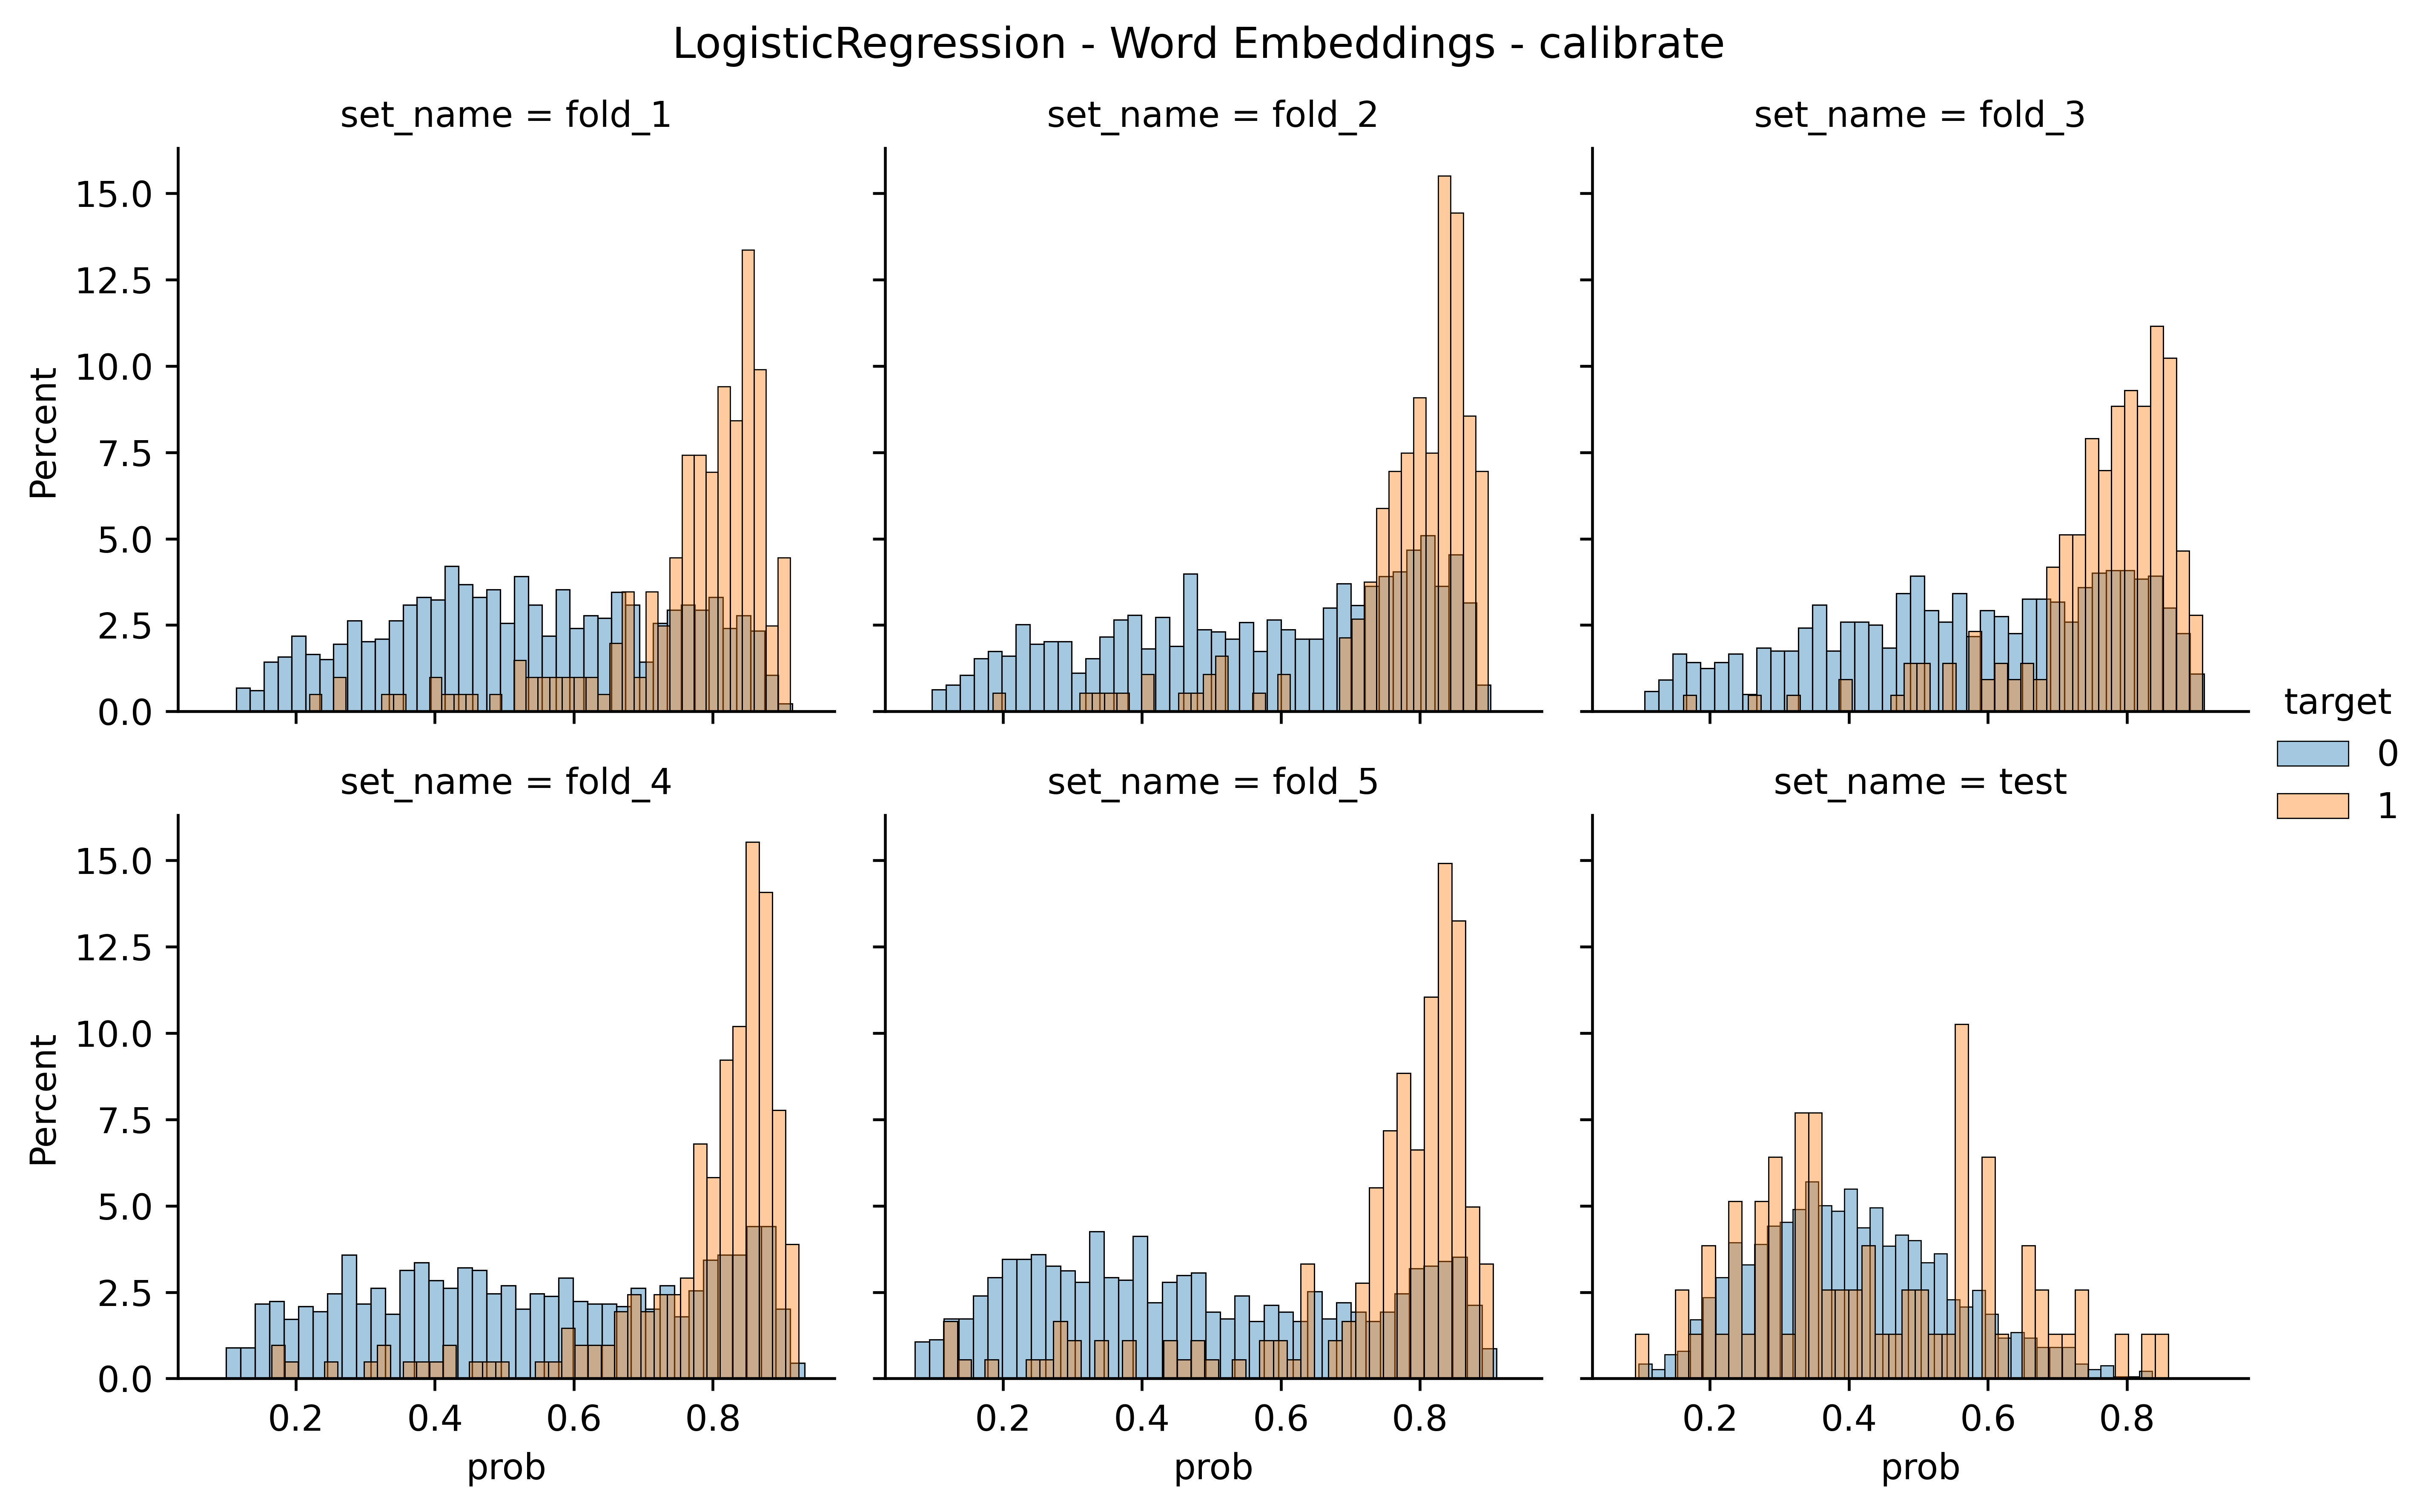
\includegraphics[width=\linewidth]{figures/results/word_embeddings/lgr/calibrate/calibrate__distplot.png}
    \end{subfigure}
    \hfill
    \centering
    \begin{subfigure}[b]{0.83\textwidth}
        \centering
        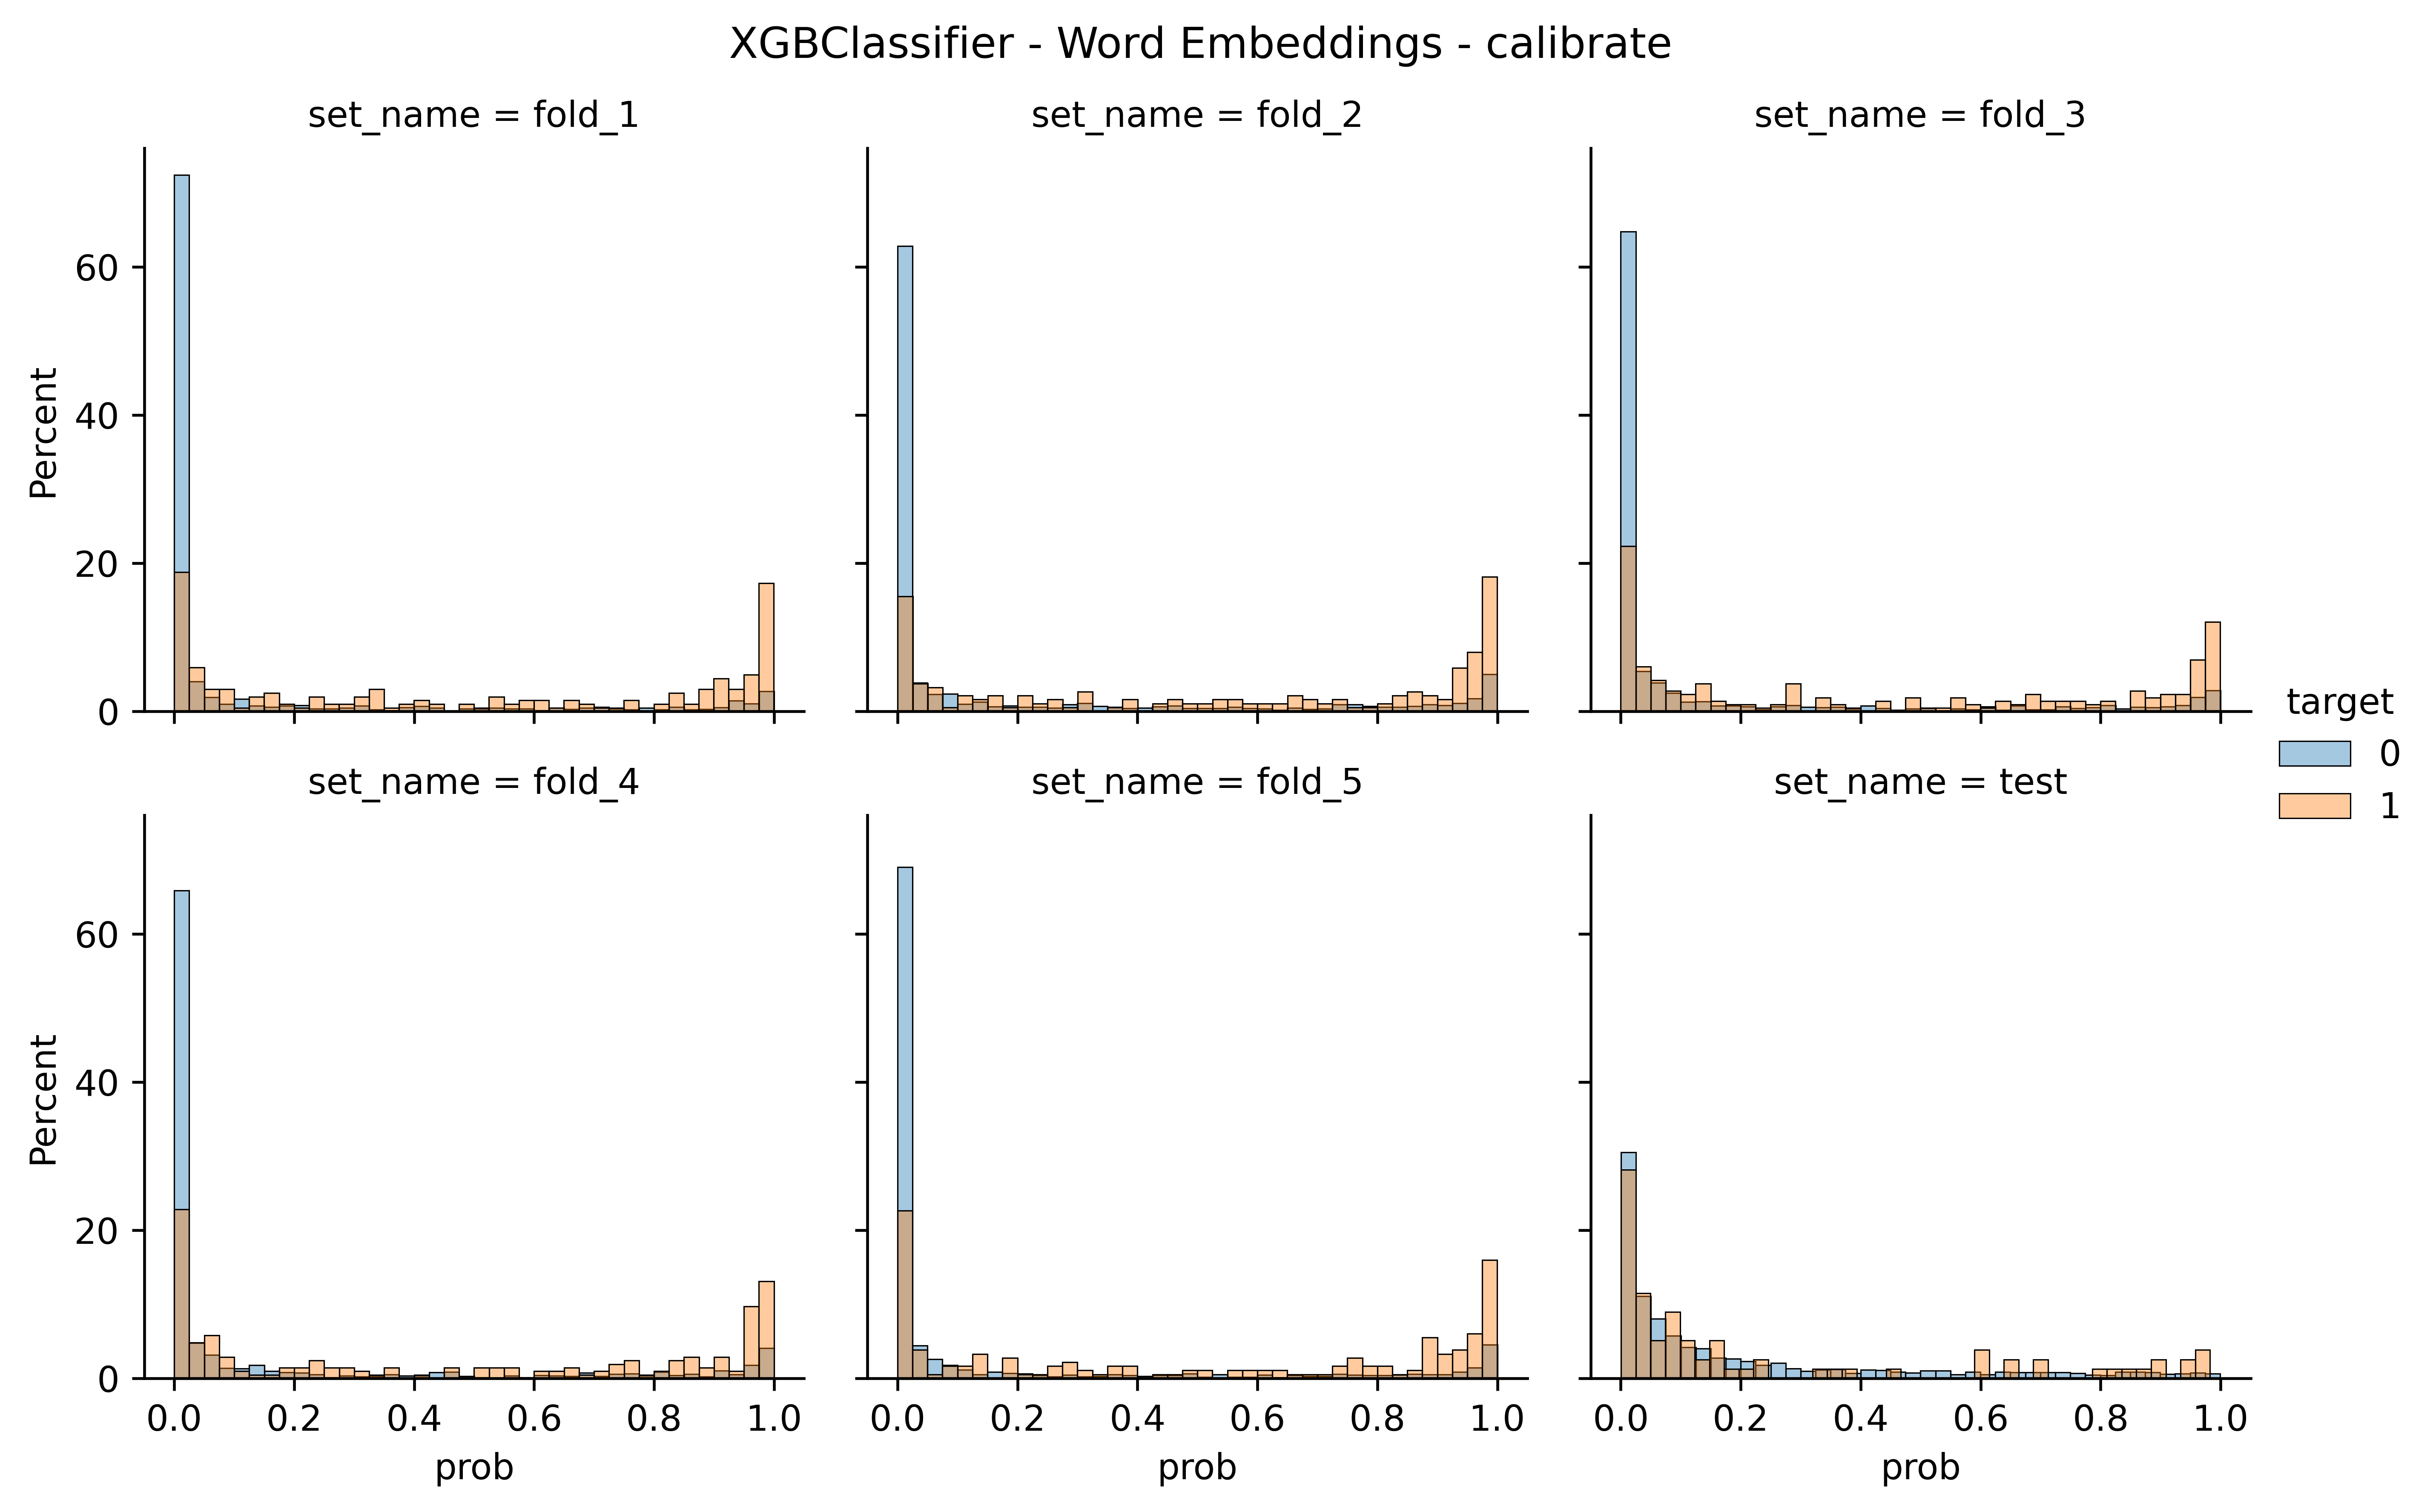
\includegraphics[width=\linewidth]{figures/results/word_embeddings/xgboost/calibrate/calibrate__distplot.png}
    \end{subfigure}
    \hfill
    \centering
    \begin{subfigure}[b]{0.83\textwidth}
        \centering
        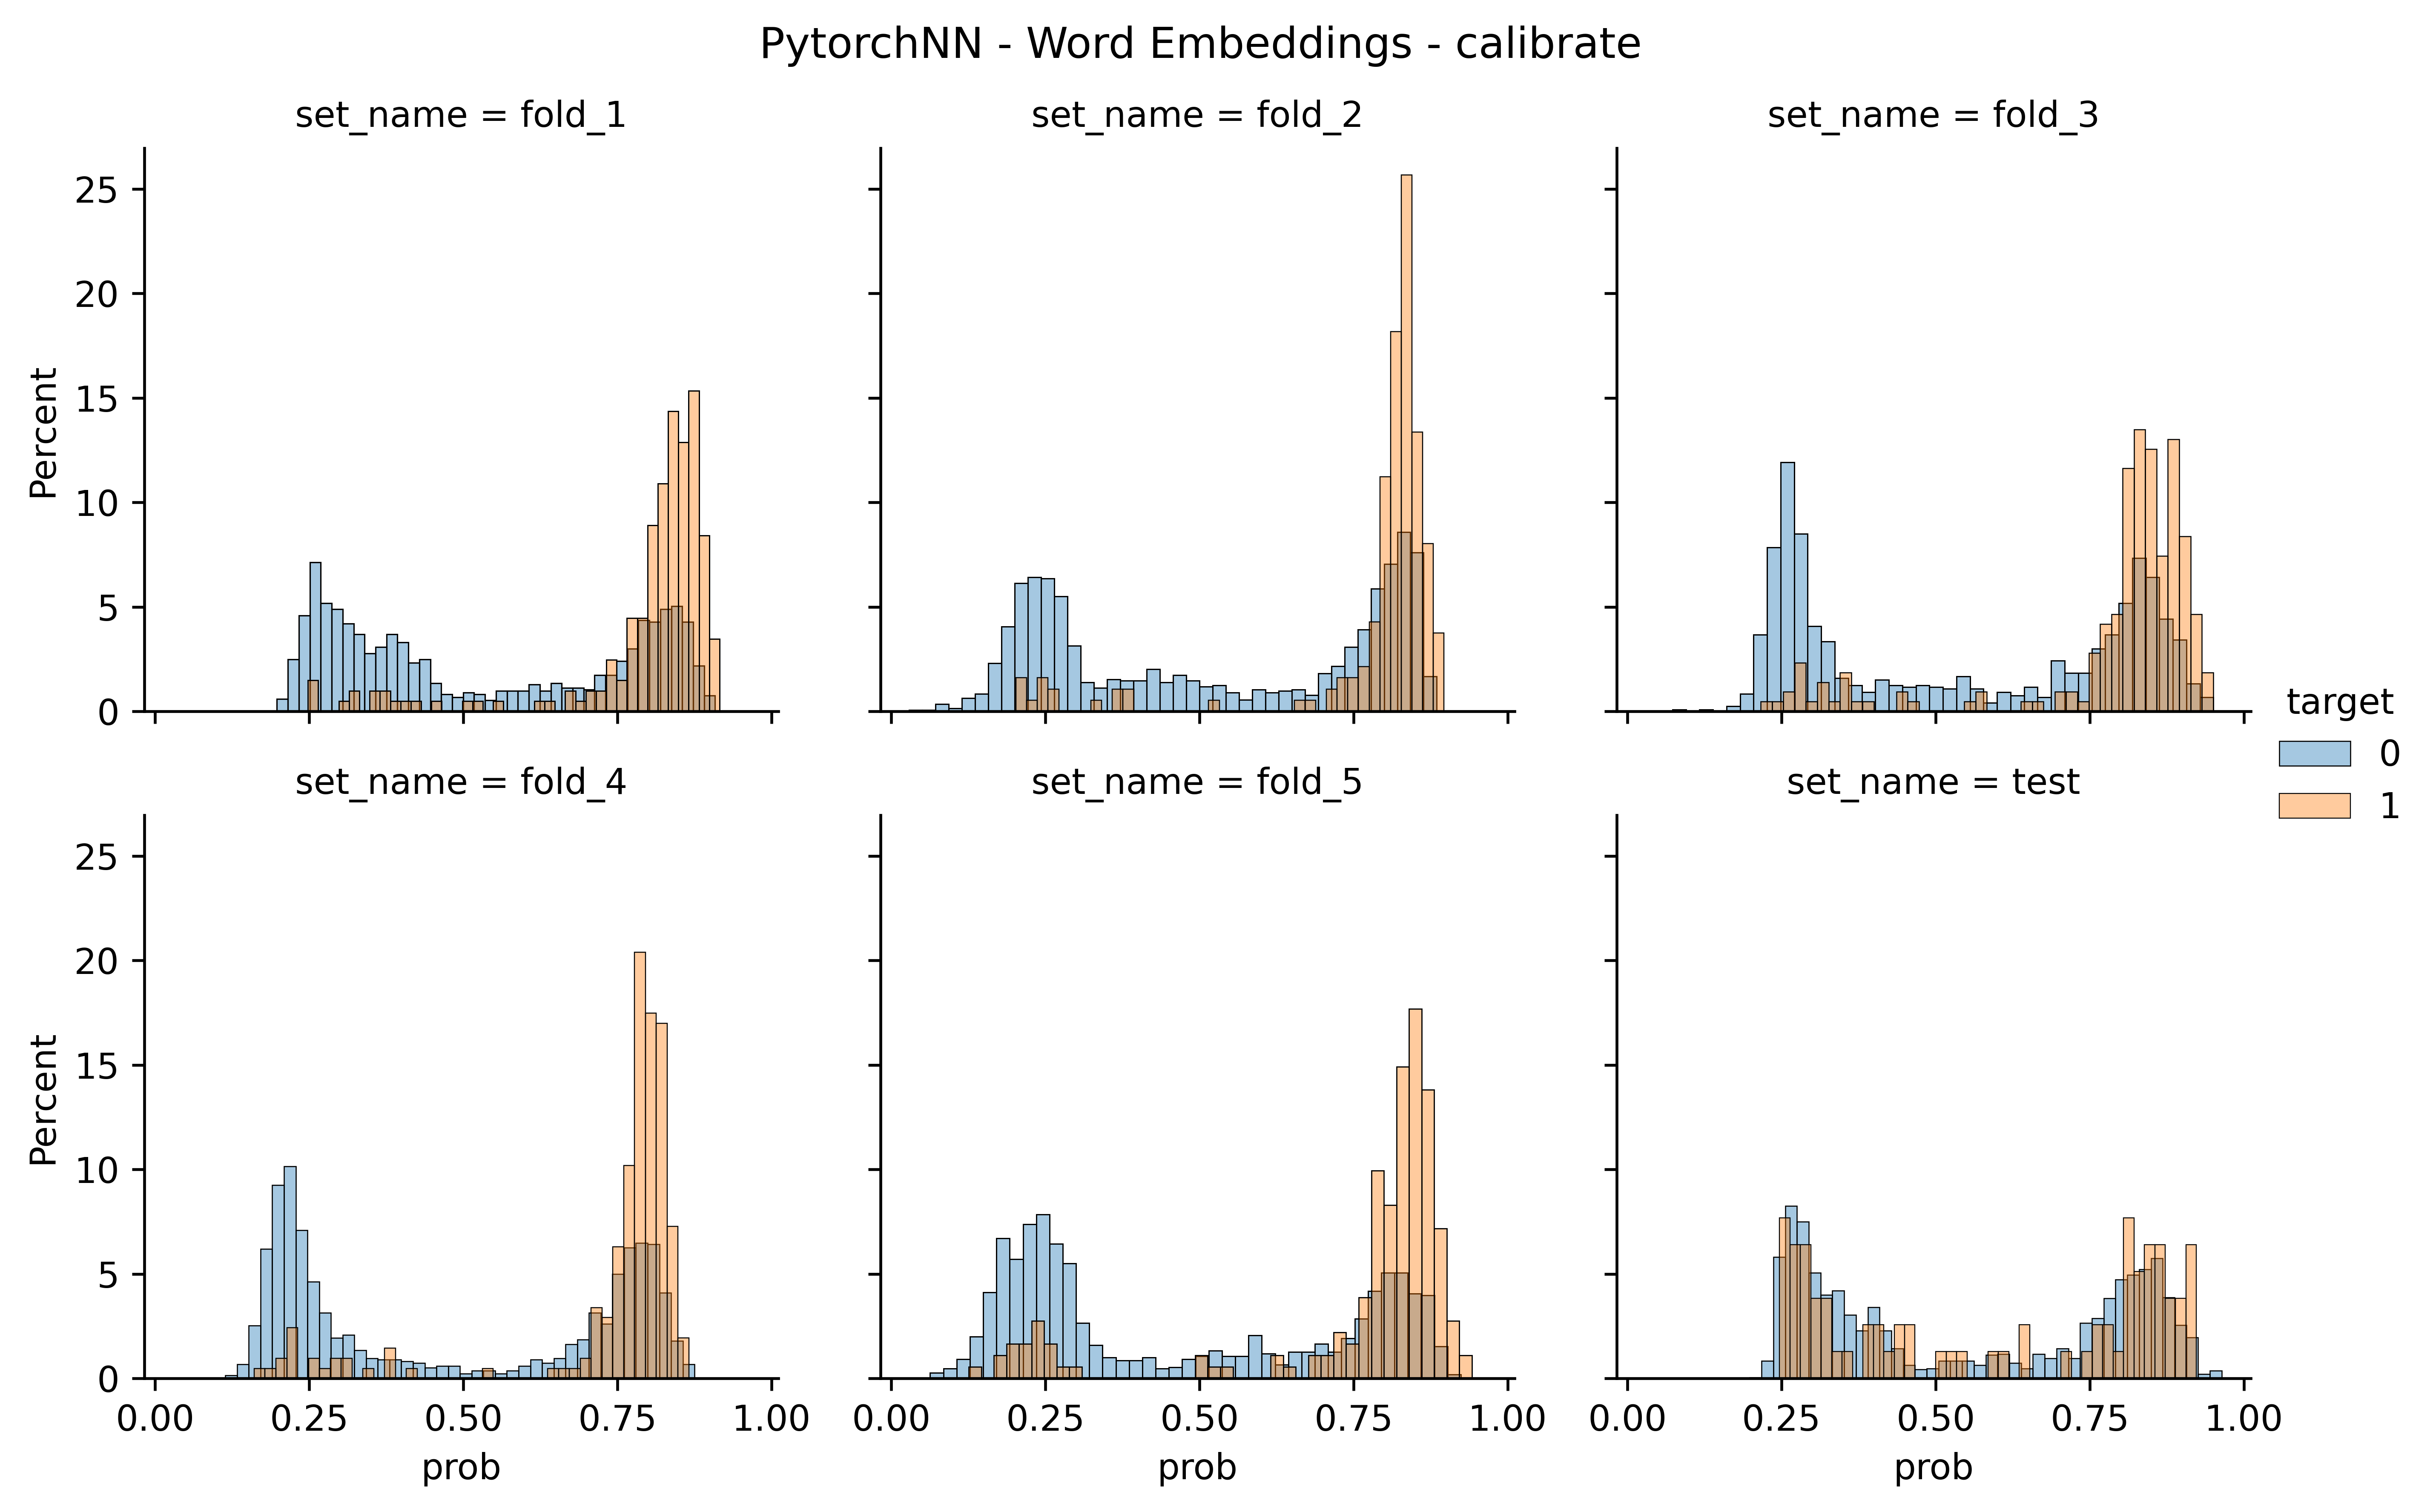
\includegraphics[width=\linewidth]{figures/results/word_embeddings/nn/calibrate/calibrate__distplot.png}
    \end{subfigure}
    \caption{Word embeddings calibrate}
\end{figure}

\begin{figure}
    \centering
    \begin{subfigure}[b]{0.83\textwidth}
    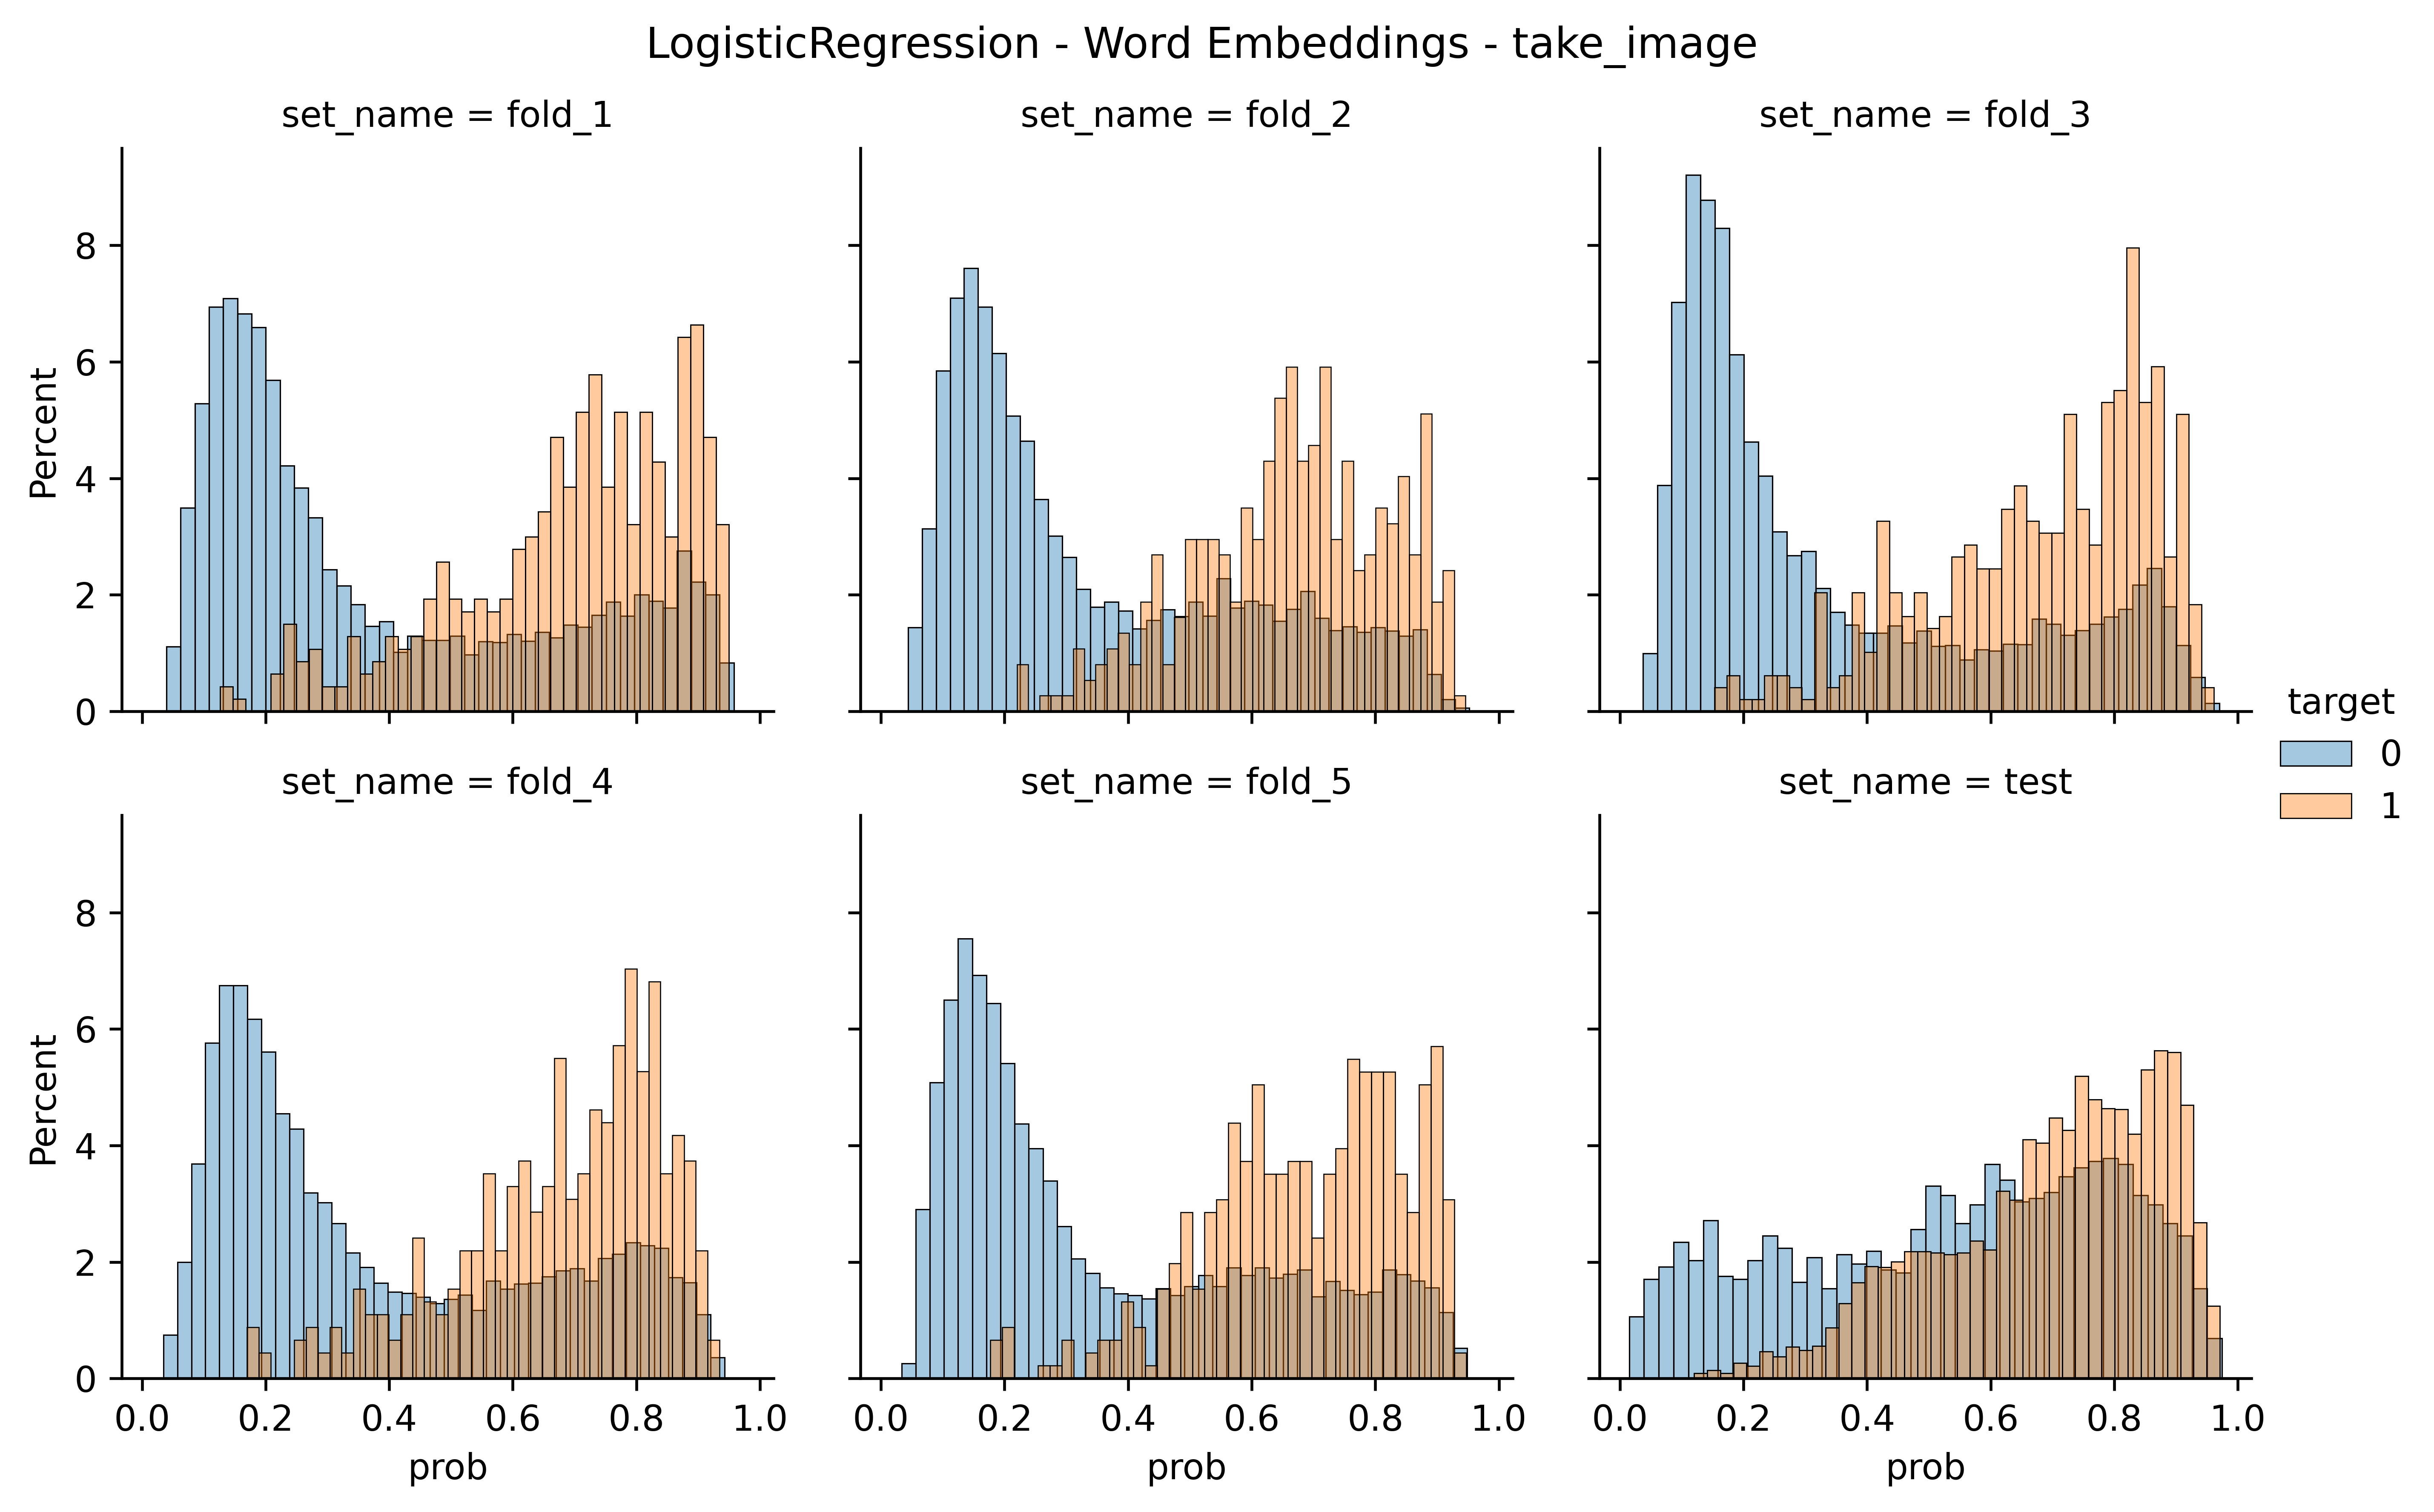
\includegraphics[width=\linewidth]{figures/results/word_embeddings/lgr/take_image/lgr__distplot.png}
    \end{subfigure}
    \hfill
    \centering
    \begin{subfigure}[b]{0.83\textwidth}
        \centering
        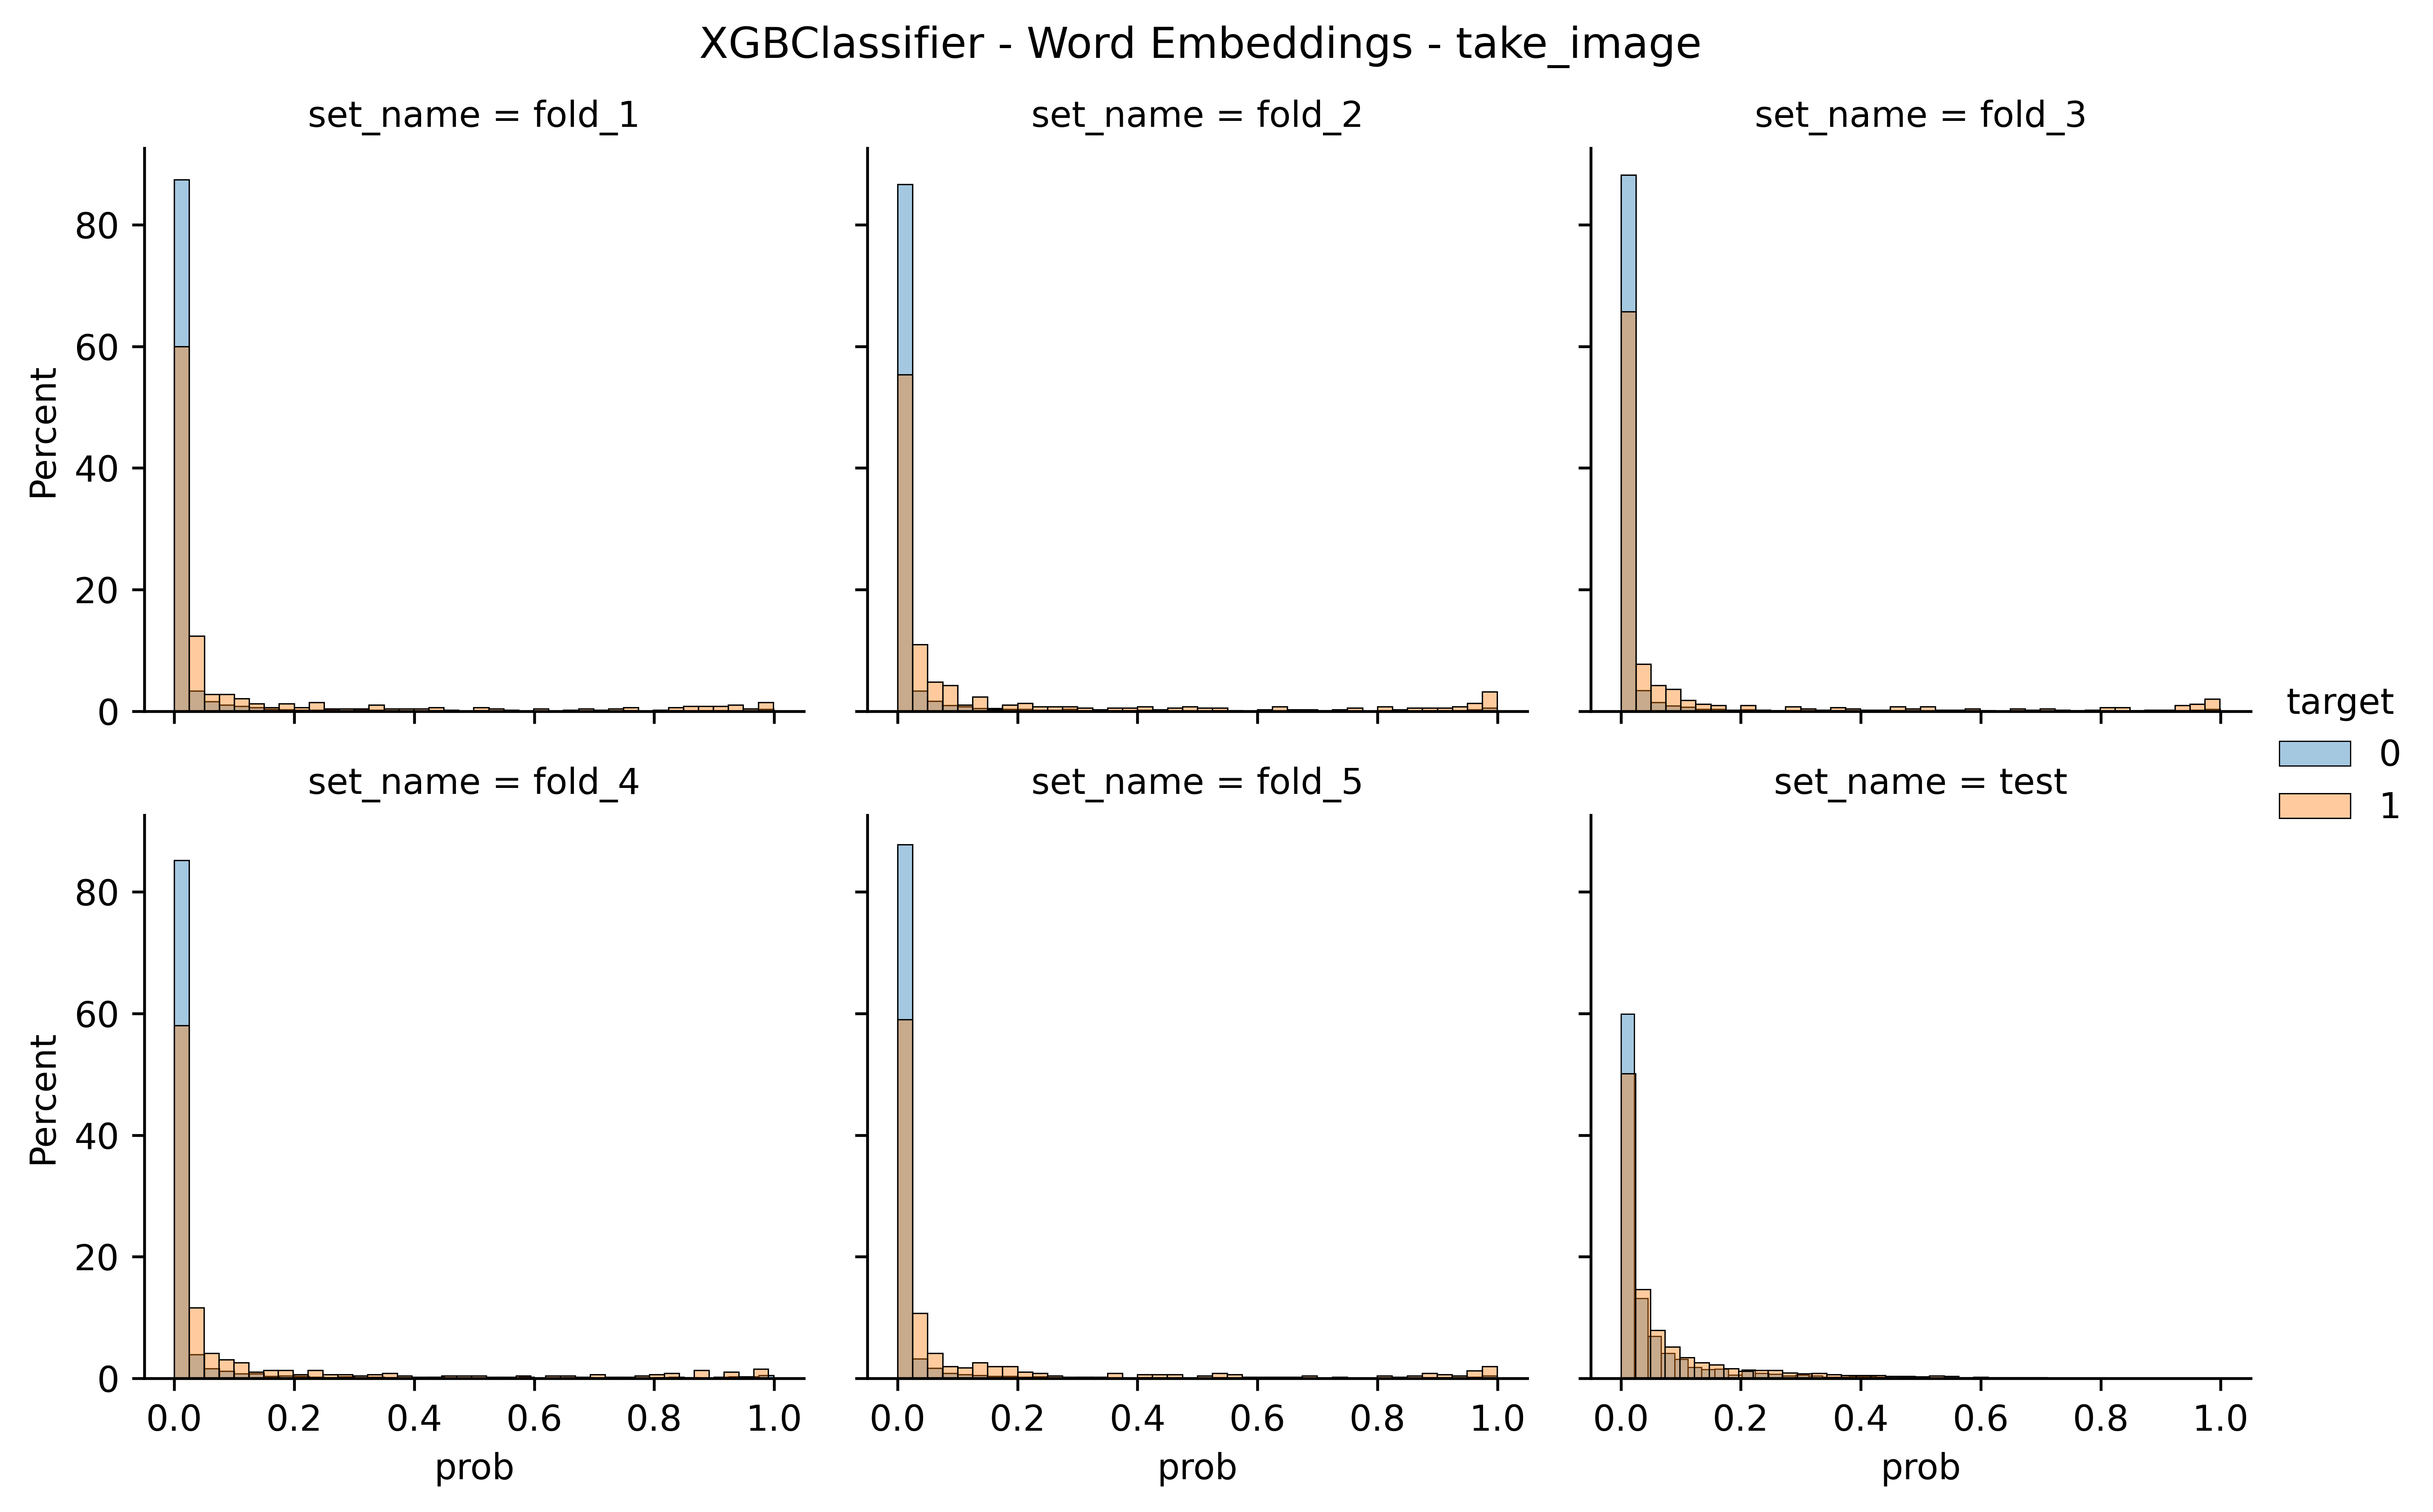
\includegraphics[width=\linewidth]{figures/results/word_embeddings/xgboost/take_image/take_image__distplot.png}
    \end{subfigure}
    \hfill
    \centering
    \begin{subfigure}[b]{0.83\textwidth}
        \centering
        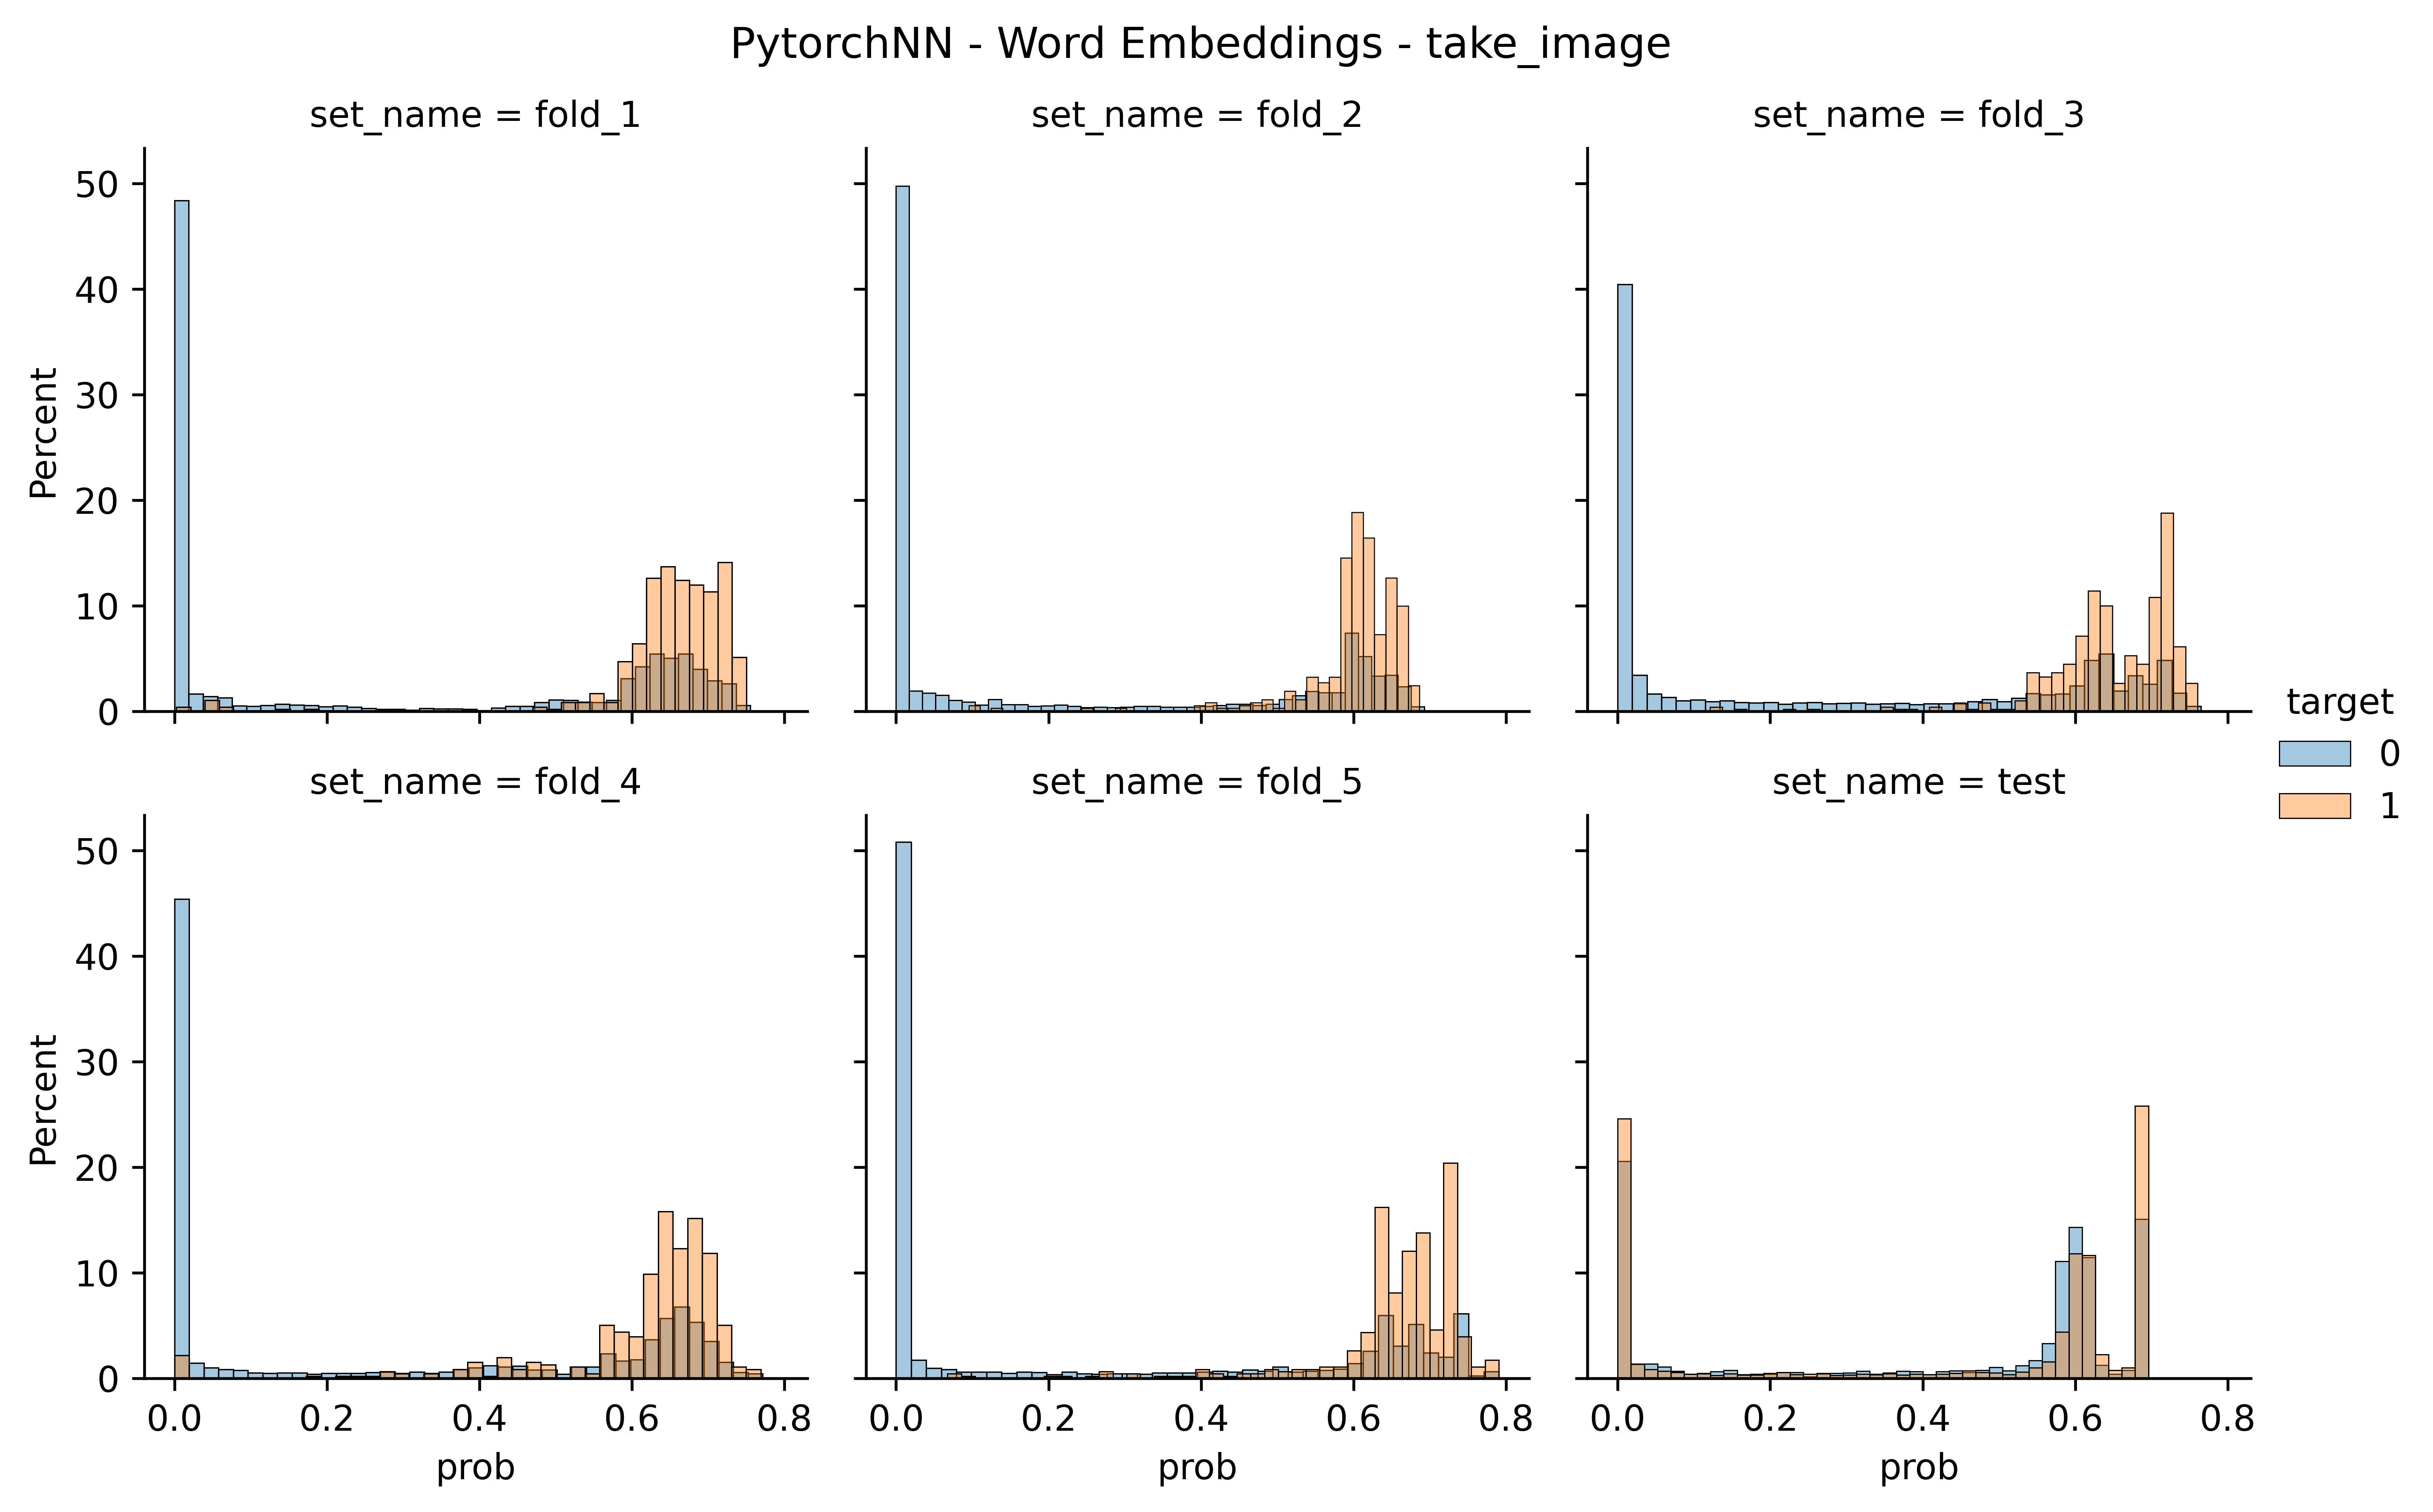
\includegraphics[width=\linewidth]{figures/results/word_embeddings/nn/take_image/take_image__distplot (1).png}
    \end{subfigure}
    \caption{Word embeddings take\_image}
\end{figure}

\begin{figure}
    \centering
    \begin{subfigure}[b]{0.83\textwidth}
    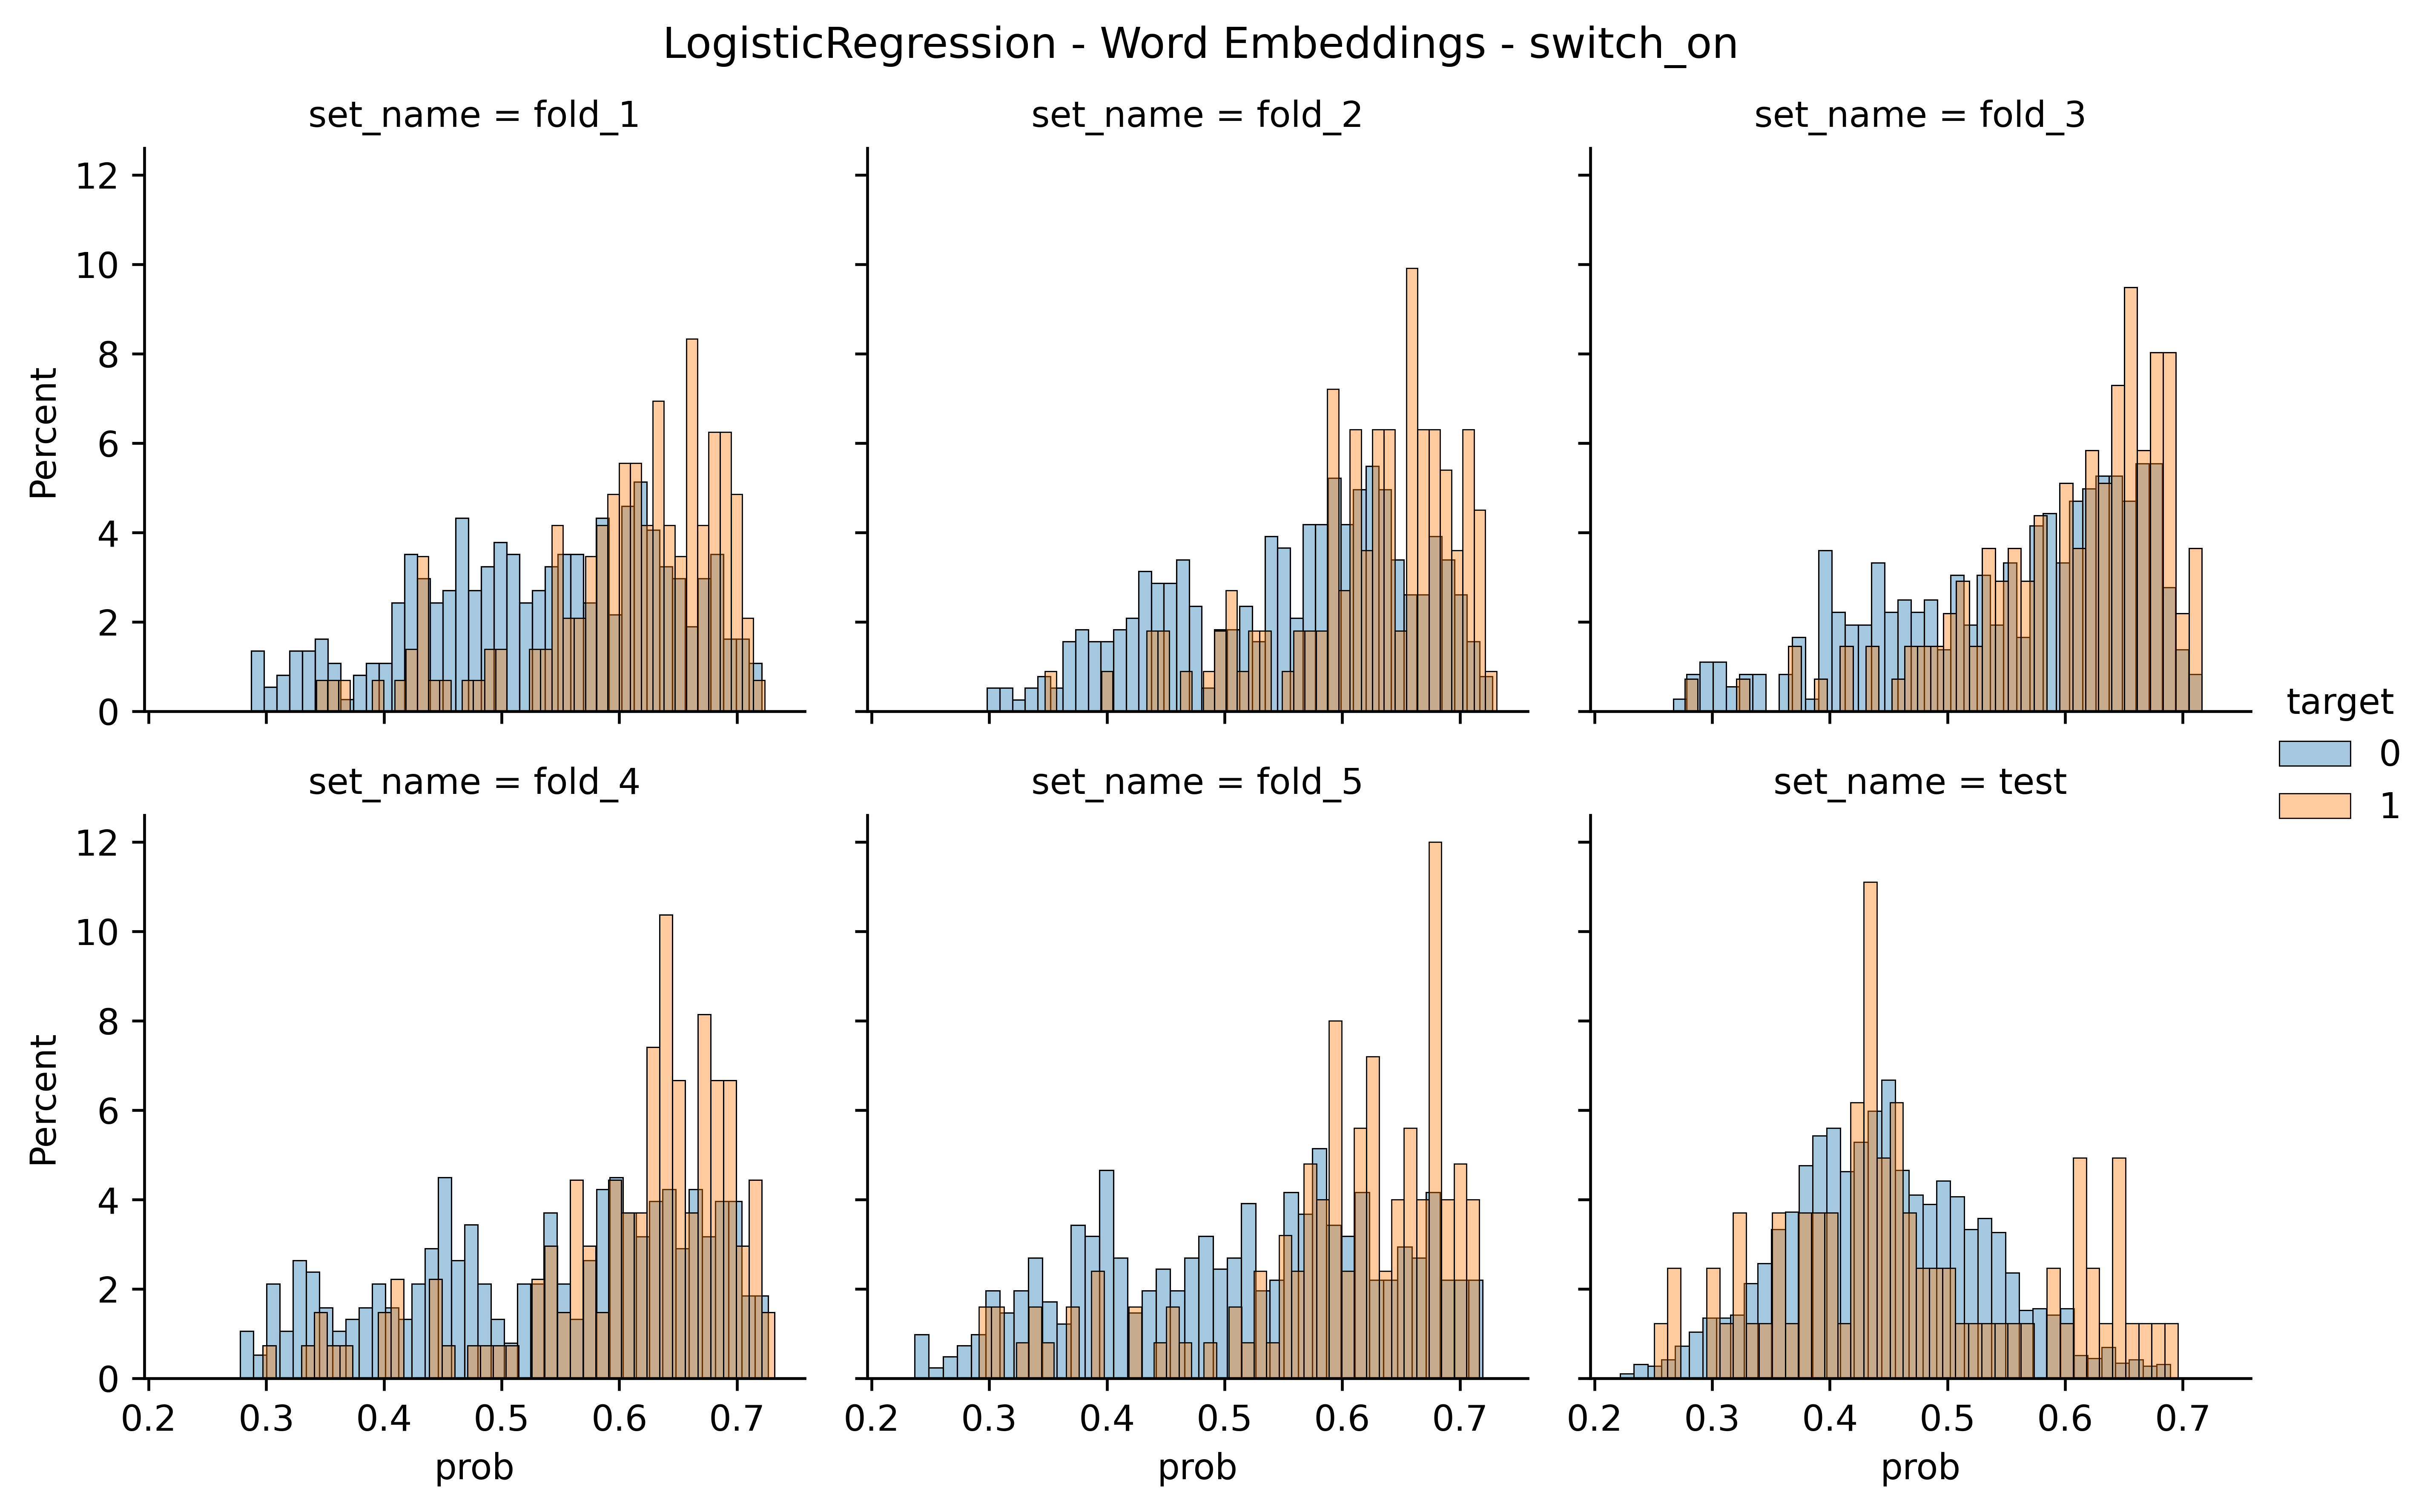
\includegraphics[width=\linewidth]{figures/results/word_embeddings/lgr/switch_on/switch_on__distplot.png}
    \end{subfigure}
    \hfill
    \centering
    \begin{subfigure}[b]{0.83\textwidth}
        \centering
        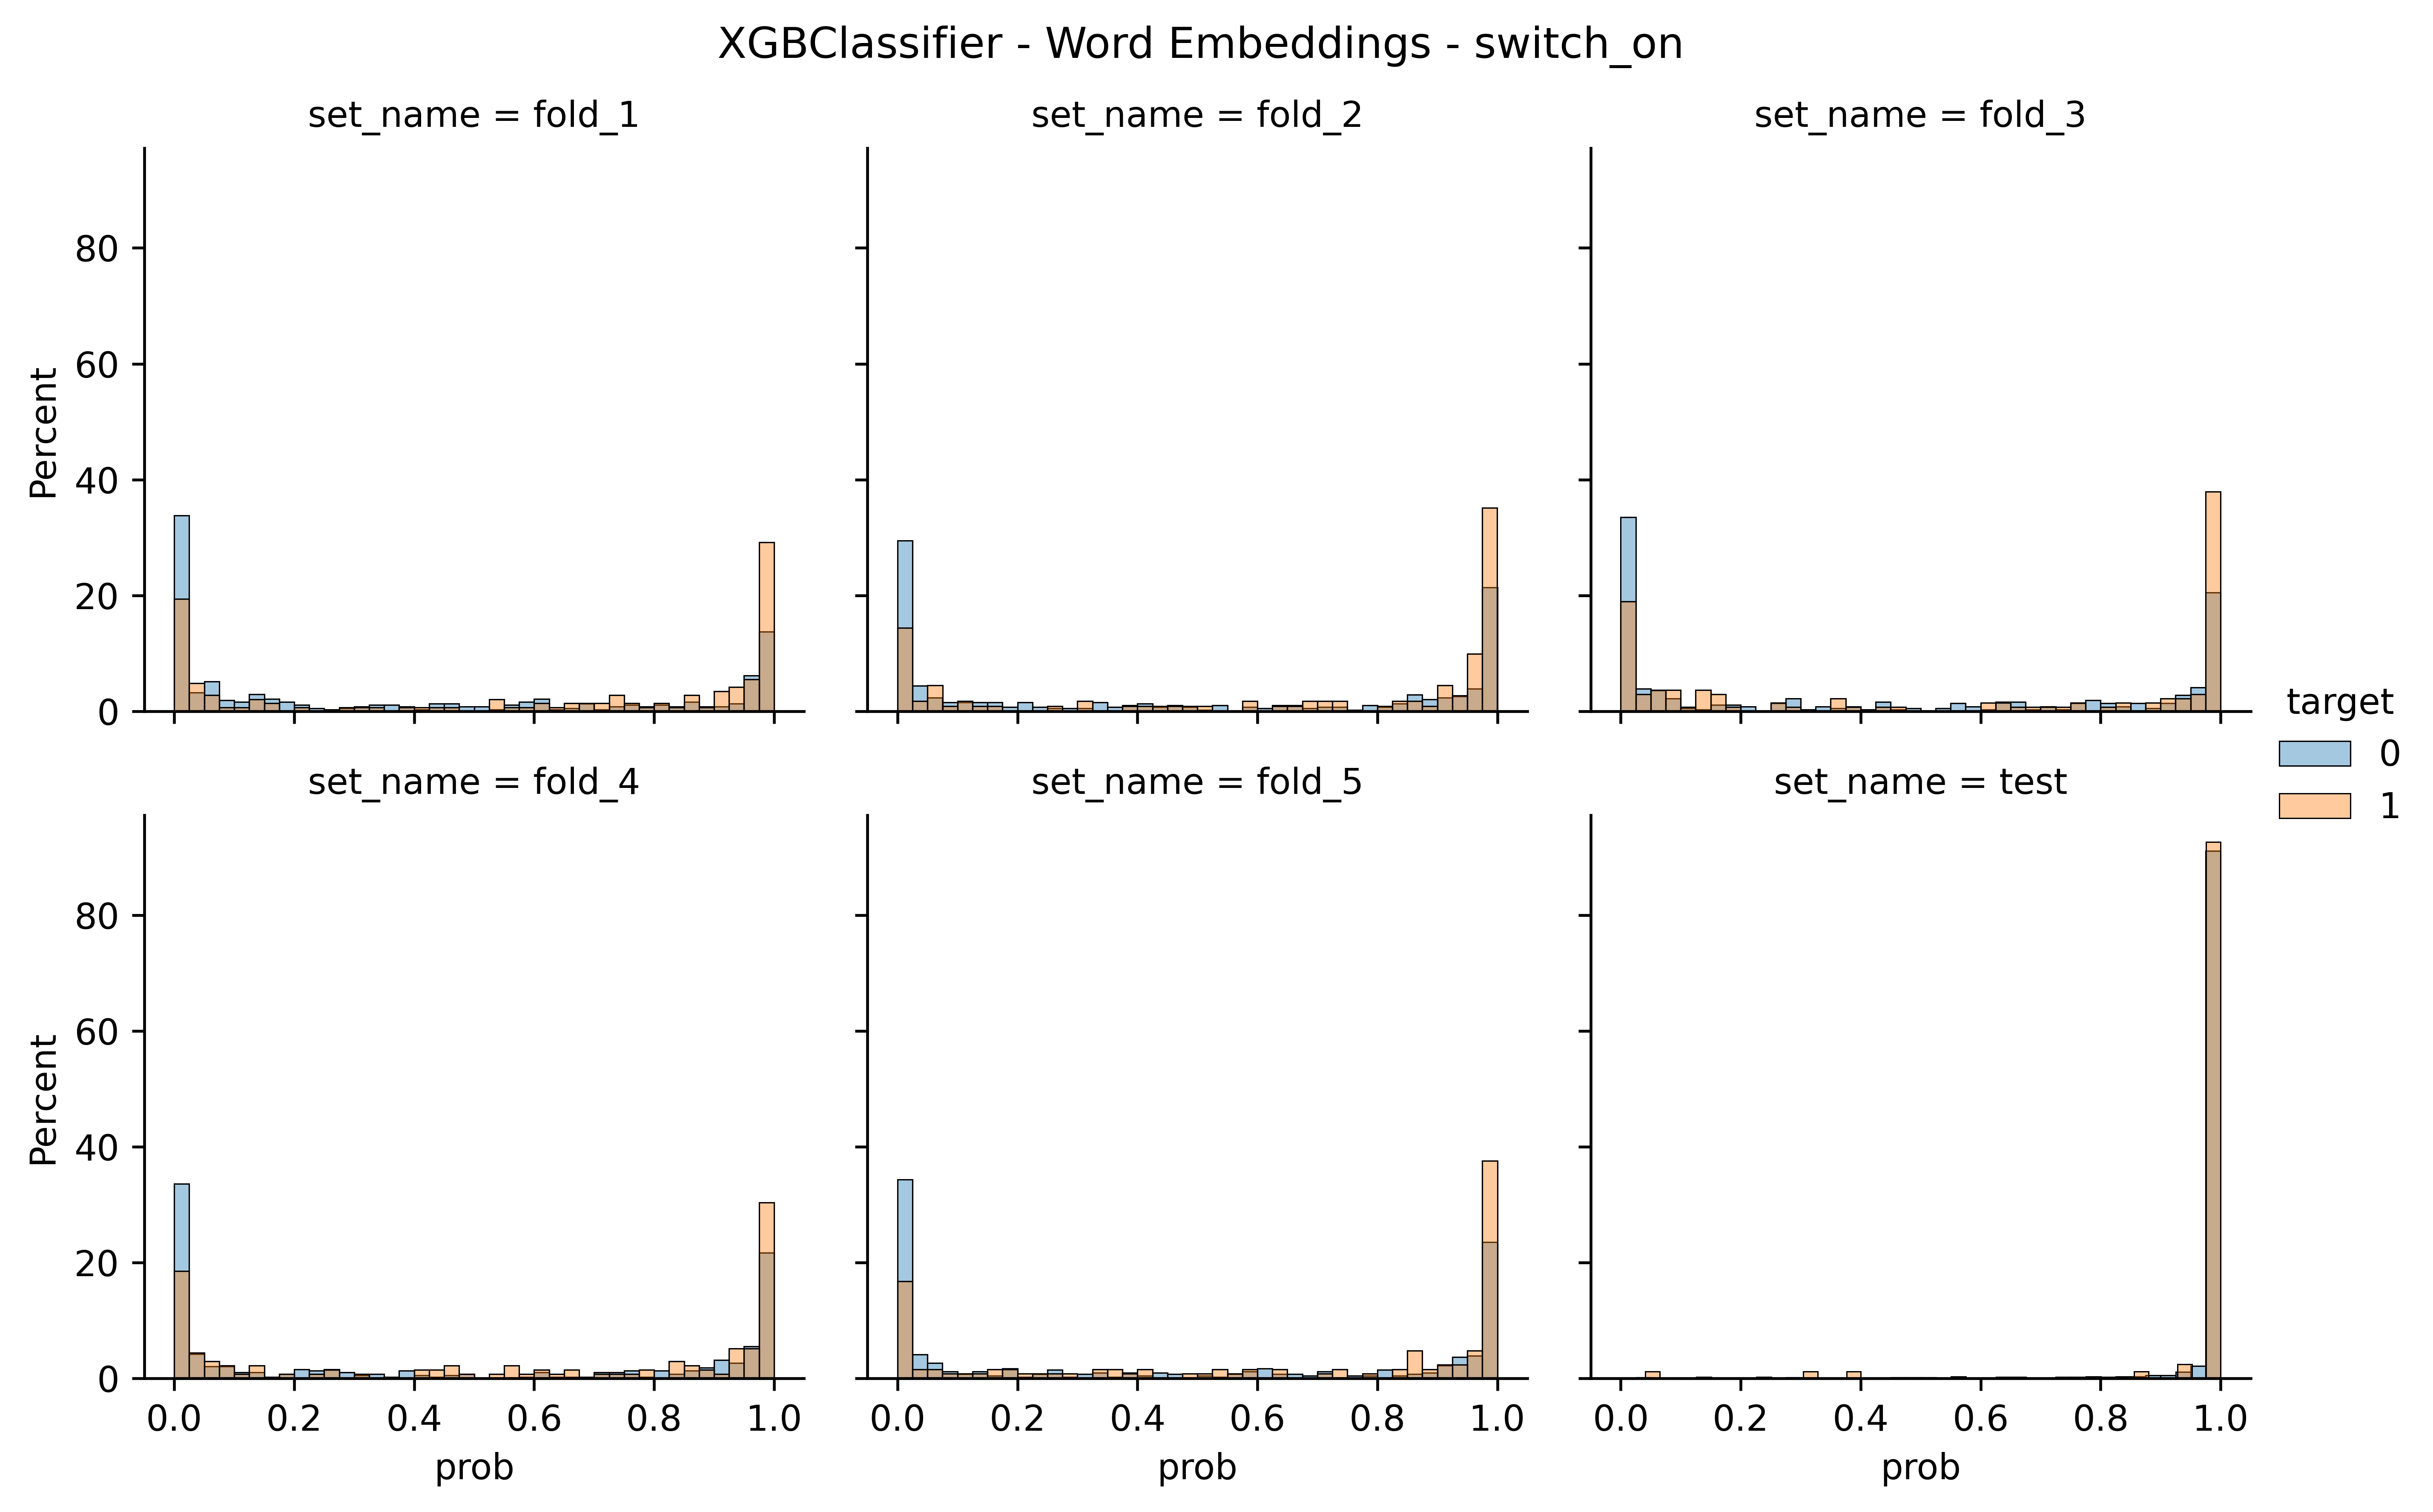
\includegraphics[width=\linewidth]{figures/results/word_embeddings/xgboost/switch_on/xgb__distplot.png}
    \end{subfigure}
    \hfill
    \centering
    \begin{subfigure}[b]{0.83\textwidth}
        \centering
        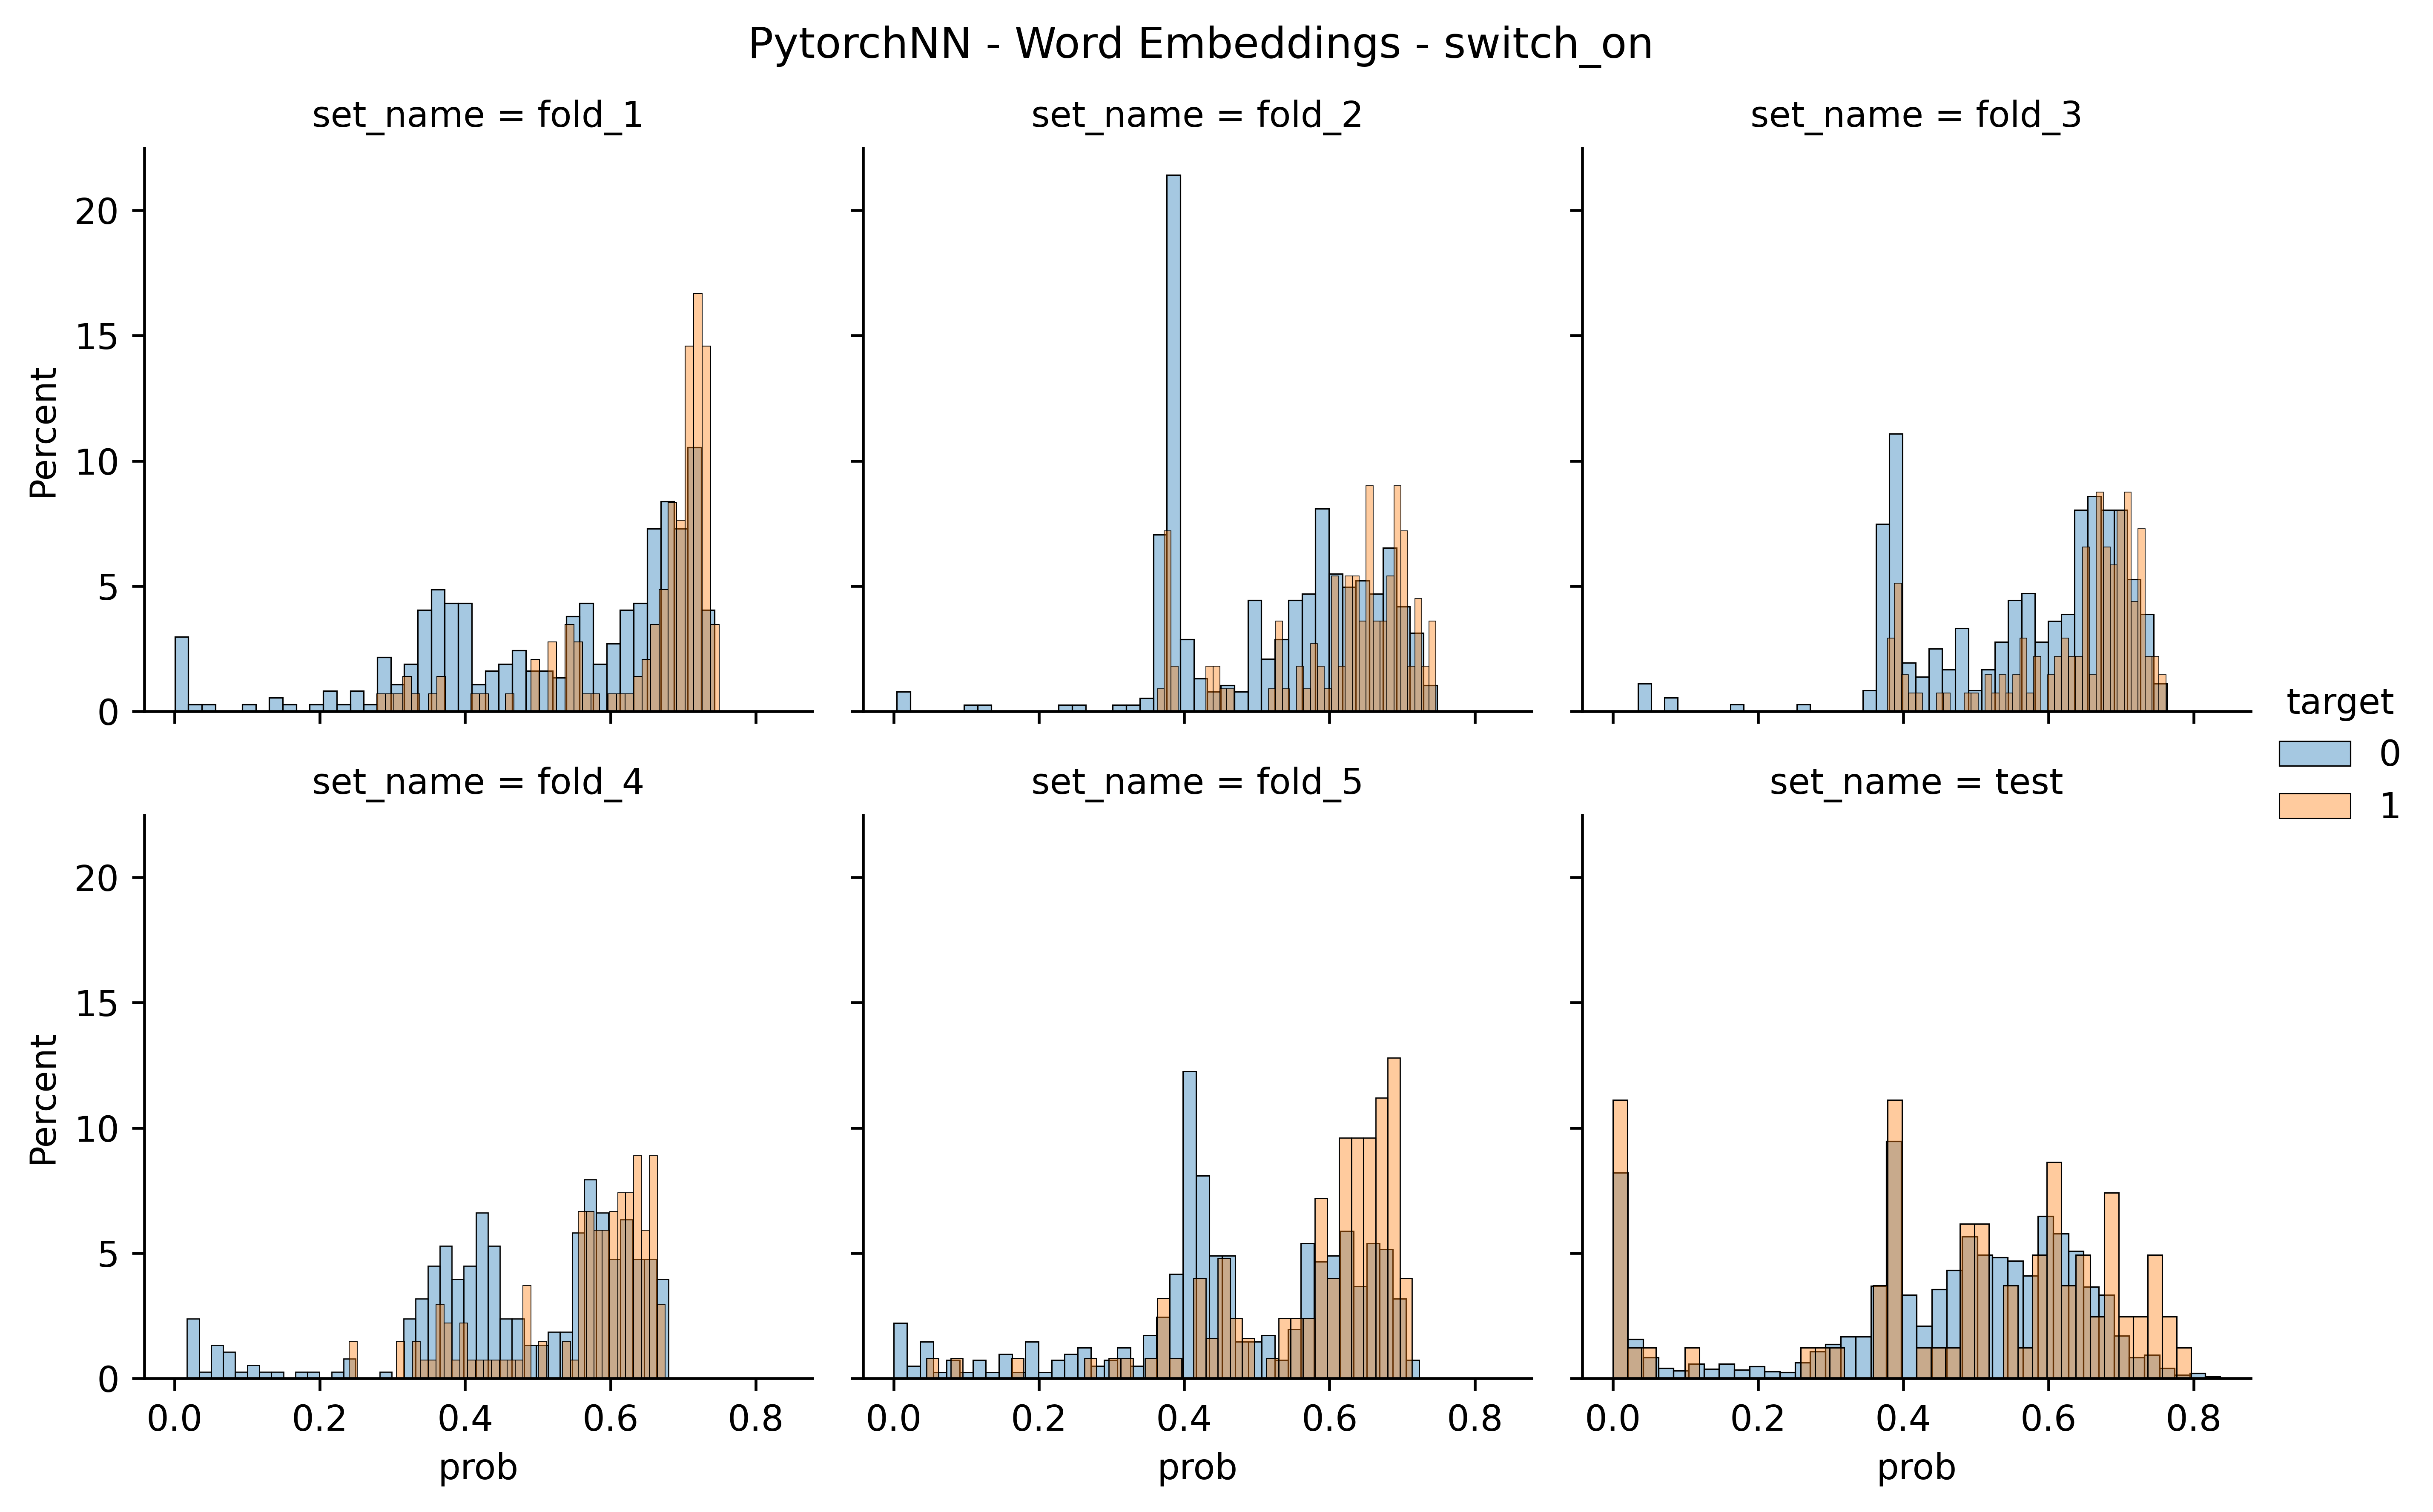
\includegraphics[width=\linewidth]{figures/results/word_embeddings/nn/switch_on/switch_on__distplot (1).png}
    \end{subfigure}
    \caption{Word embeddings switch\_on}
\end{figure}


\begin{figure}
    \begin{subfigure}[b]{\textwidth}
        \centering
        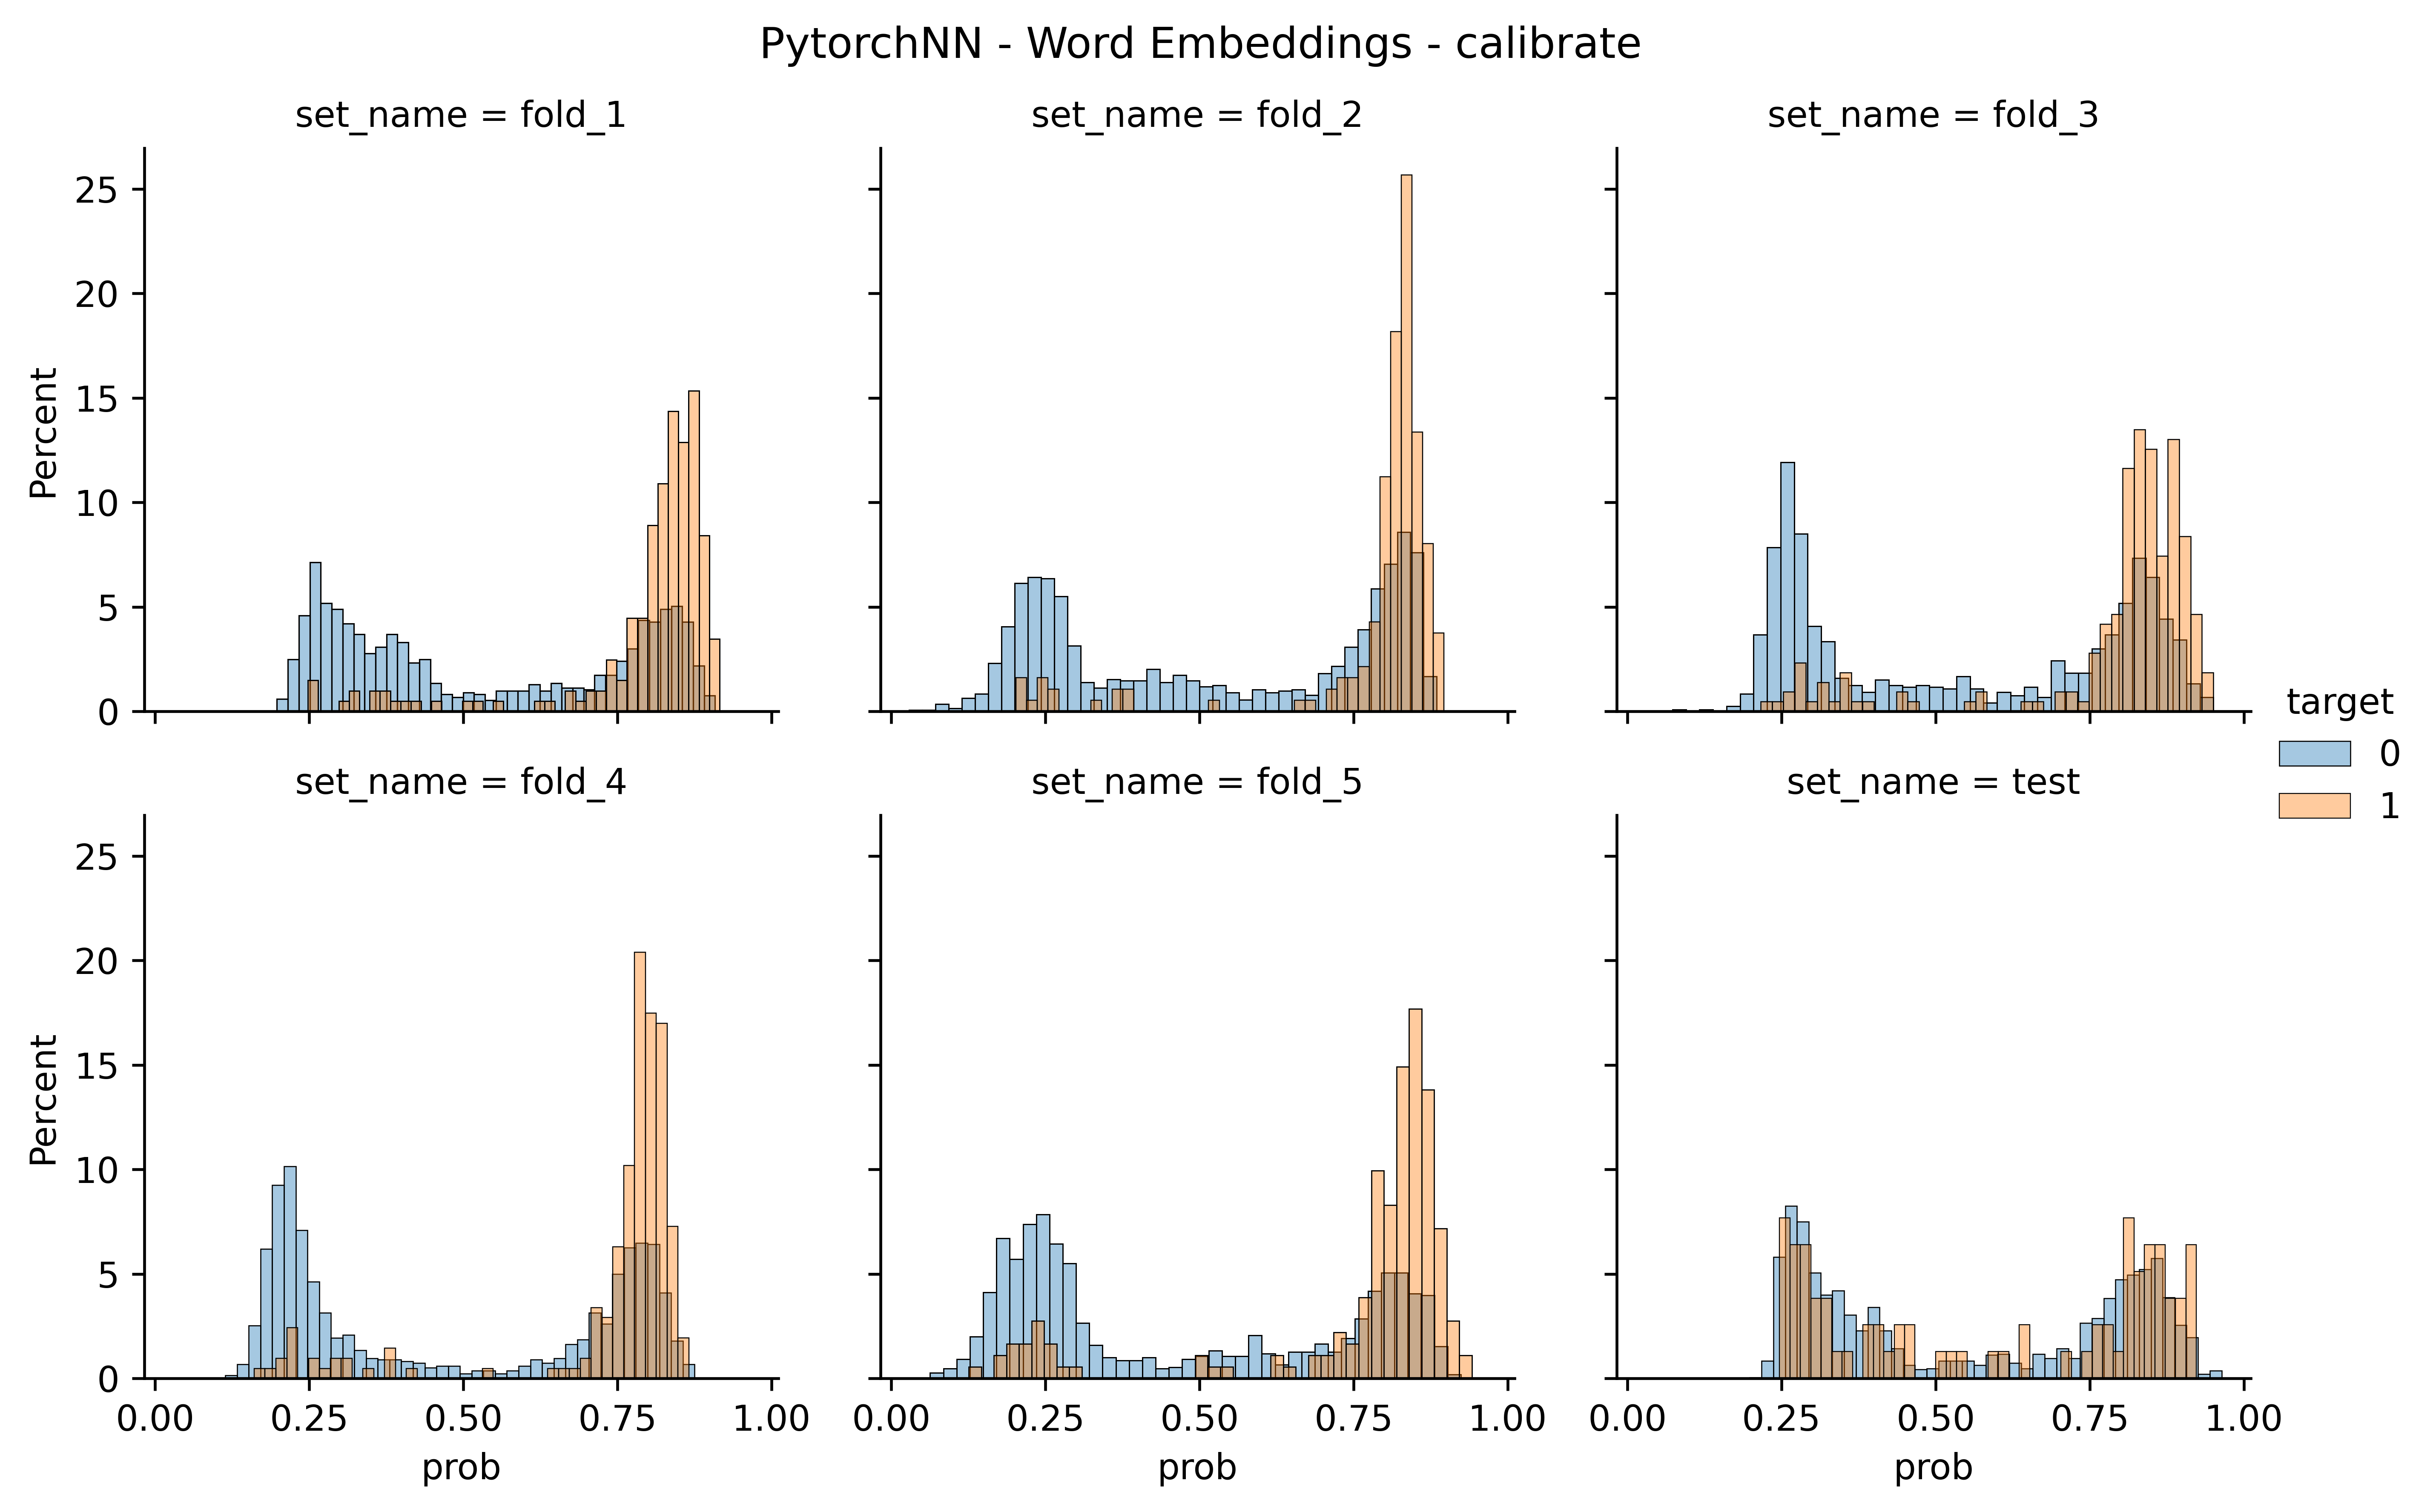
\includegraphics[width=\linewidth]{figures/results/word_embeddings/nn/calibrate/calibrate__distplot.png}
        \caption{Distribución de predicciones en validación cruzada y el conjunto de test.}
        \label{fig:my_label}
    \end{subfigure}
    \hfill
    \begin{subfigure}[b]{\textwidth}
    \minipage{0.32\textwidth}
      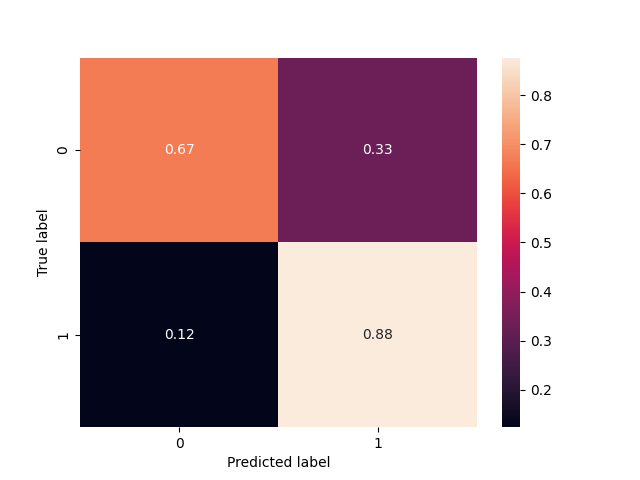
\includegraphics[width=\linewidth]{figures/results/word_embeddings/nn/calibrate/calibrate_set_1_confusion_matrix_percent.png}
    \endminipage\hfill
    \minipage{0.32\textwidth}
      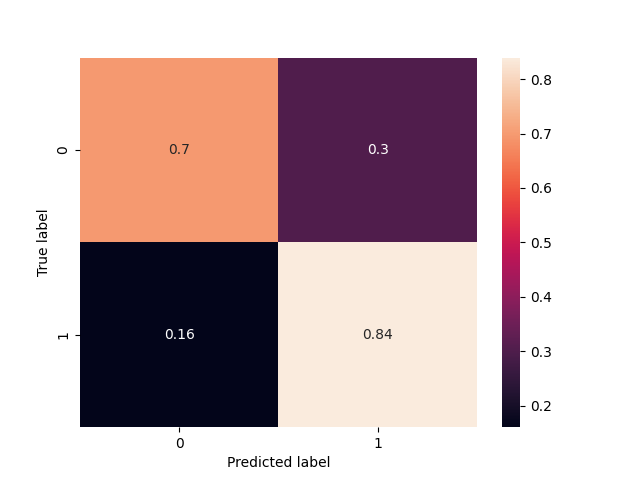
\includegraphics[width=\linewidth]{figures/results/word_embeddings/nn/calibrate/calibrate_set_2_confusion_matrix_percent.png}
    \endminipage\hfill
    \minipage{0.32\textwidth}%
      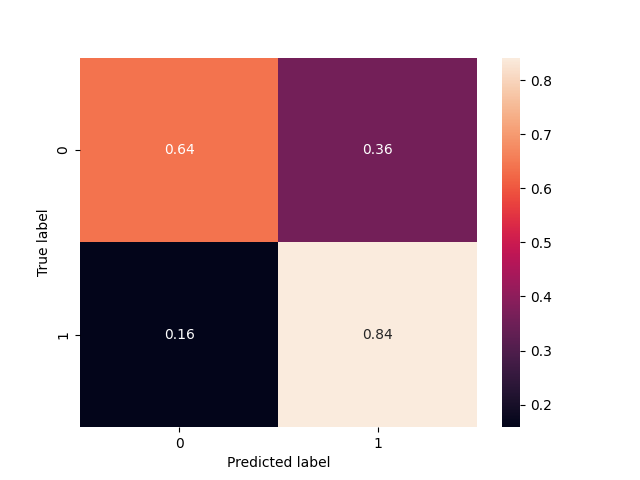
\includegraphics[width=\linewidth]{figures/results/word_embeddings/nn/calibrate/calibrate+_set_3_confusion_matrix_percent.png}
    \endminipage
    
    \medskip
    
    \minipage{0.32\textwidth}
      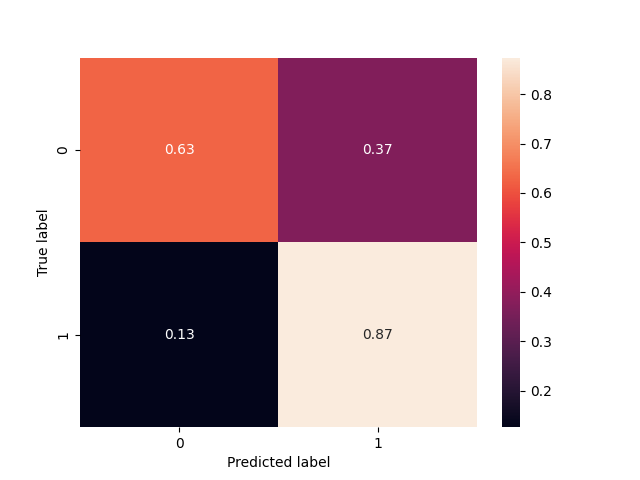
\includegraphics[width=\linewidth]{figures/results/word_embeddings/nn/calibrate/calibrate_set_4_confusion_matrix_percent.png}
    \endminipage\hfill
    \minipage{0.32\textwidth}
    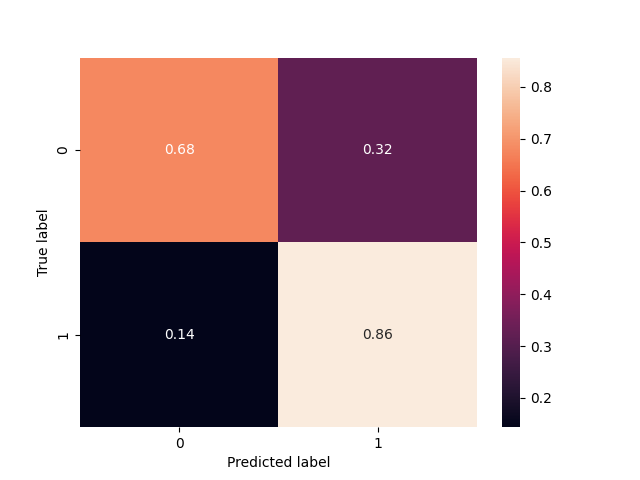
\includegraphics[width=\linewidth]{figures/results/word_embeddings/nn/calibrate/calibrate_set_5_confusion_matrix_percent.png}
    \endminipage\hfill
    \minipage{0.32\textwidth}%
    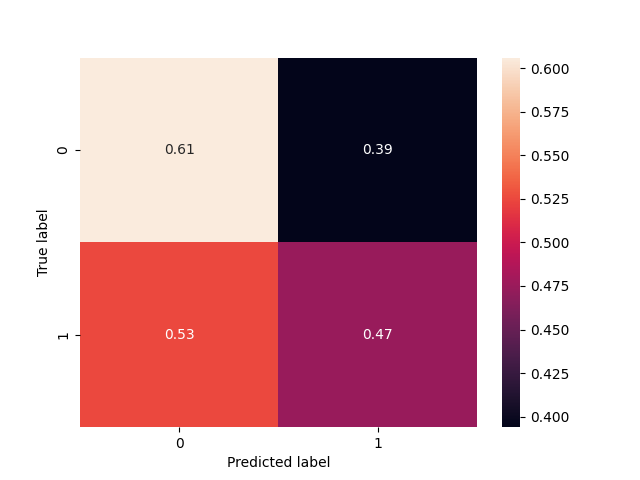
\includegraphics[width=\linewidth]{figures/results/word_embeddings/nn/calibrate/calibrate_set_6_confusion_matrix_percent.png}
    \endminipage
    \caption{Matrices de confusión en validación cruzada y el conjunto de test}
    \end{subfigure}
    \caption{Resultados del modelo de redes neuronales con codificación por word embeddings y esquema de acción calibrate.}
\end{figure}


\begin{figure}
    \begin{subfigure}[b]{\textwidth}
        \centering
        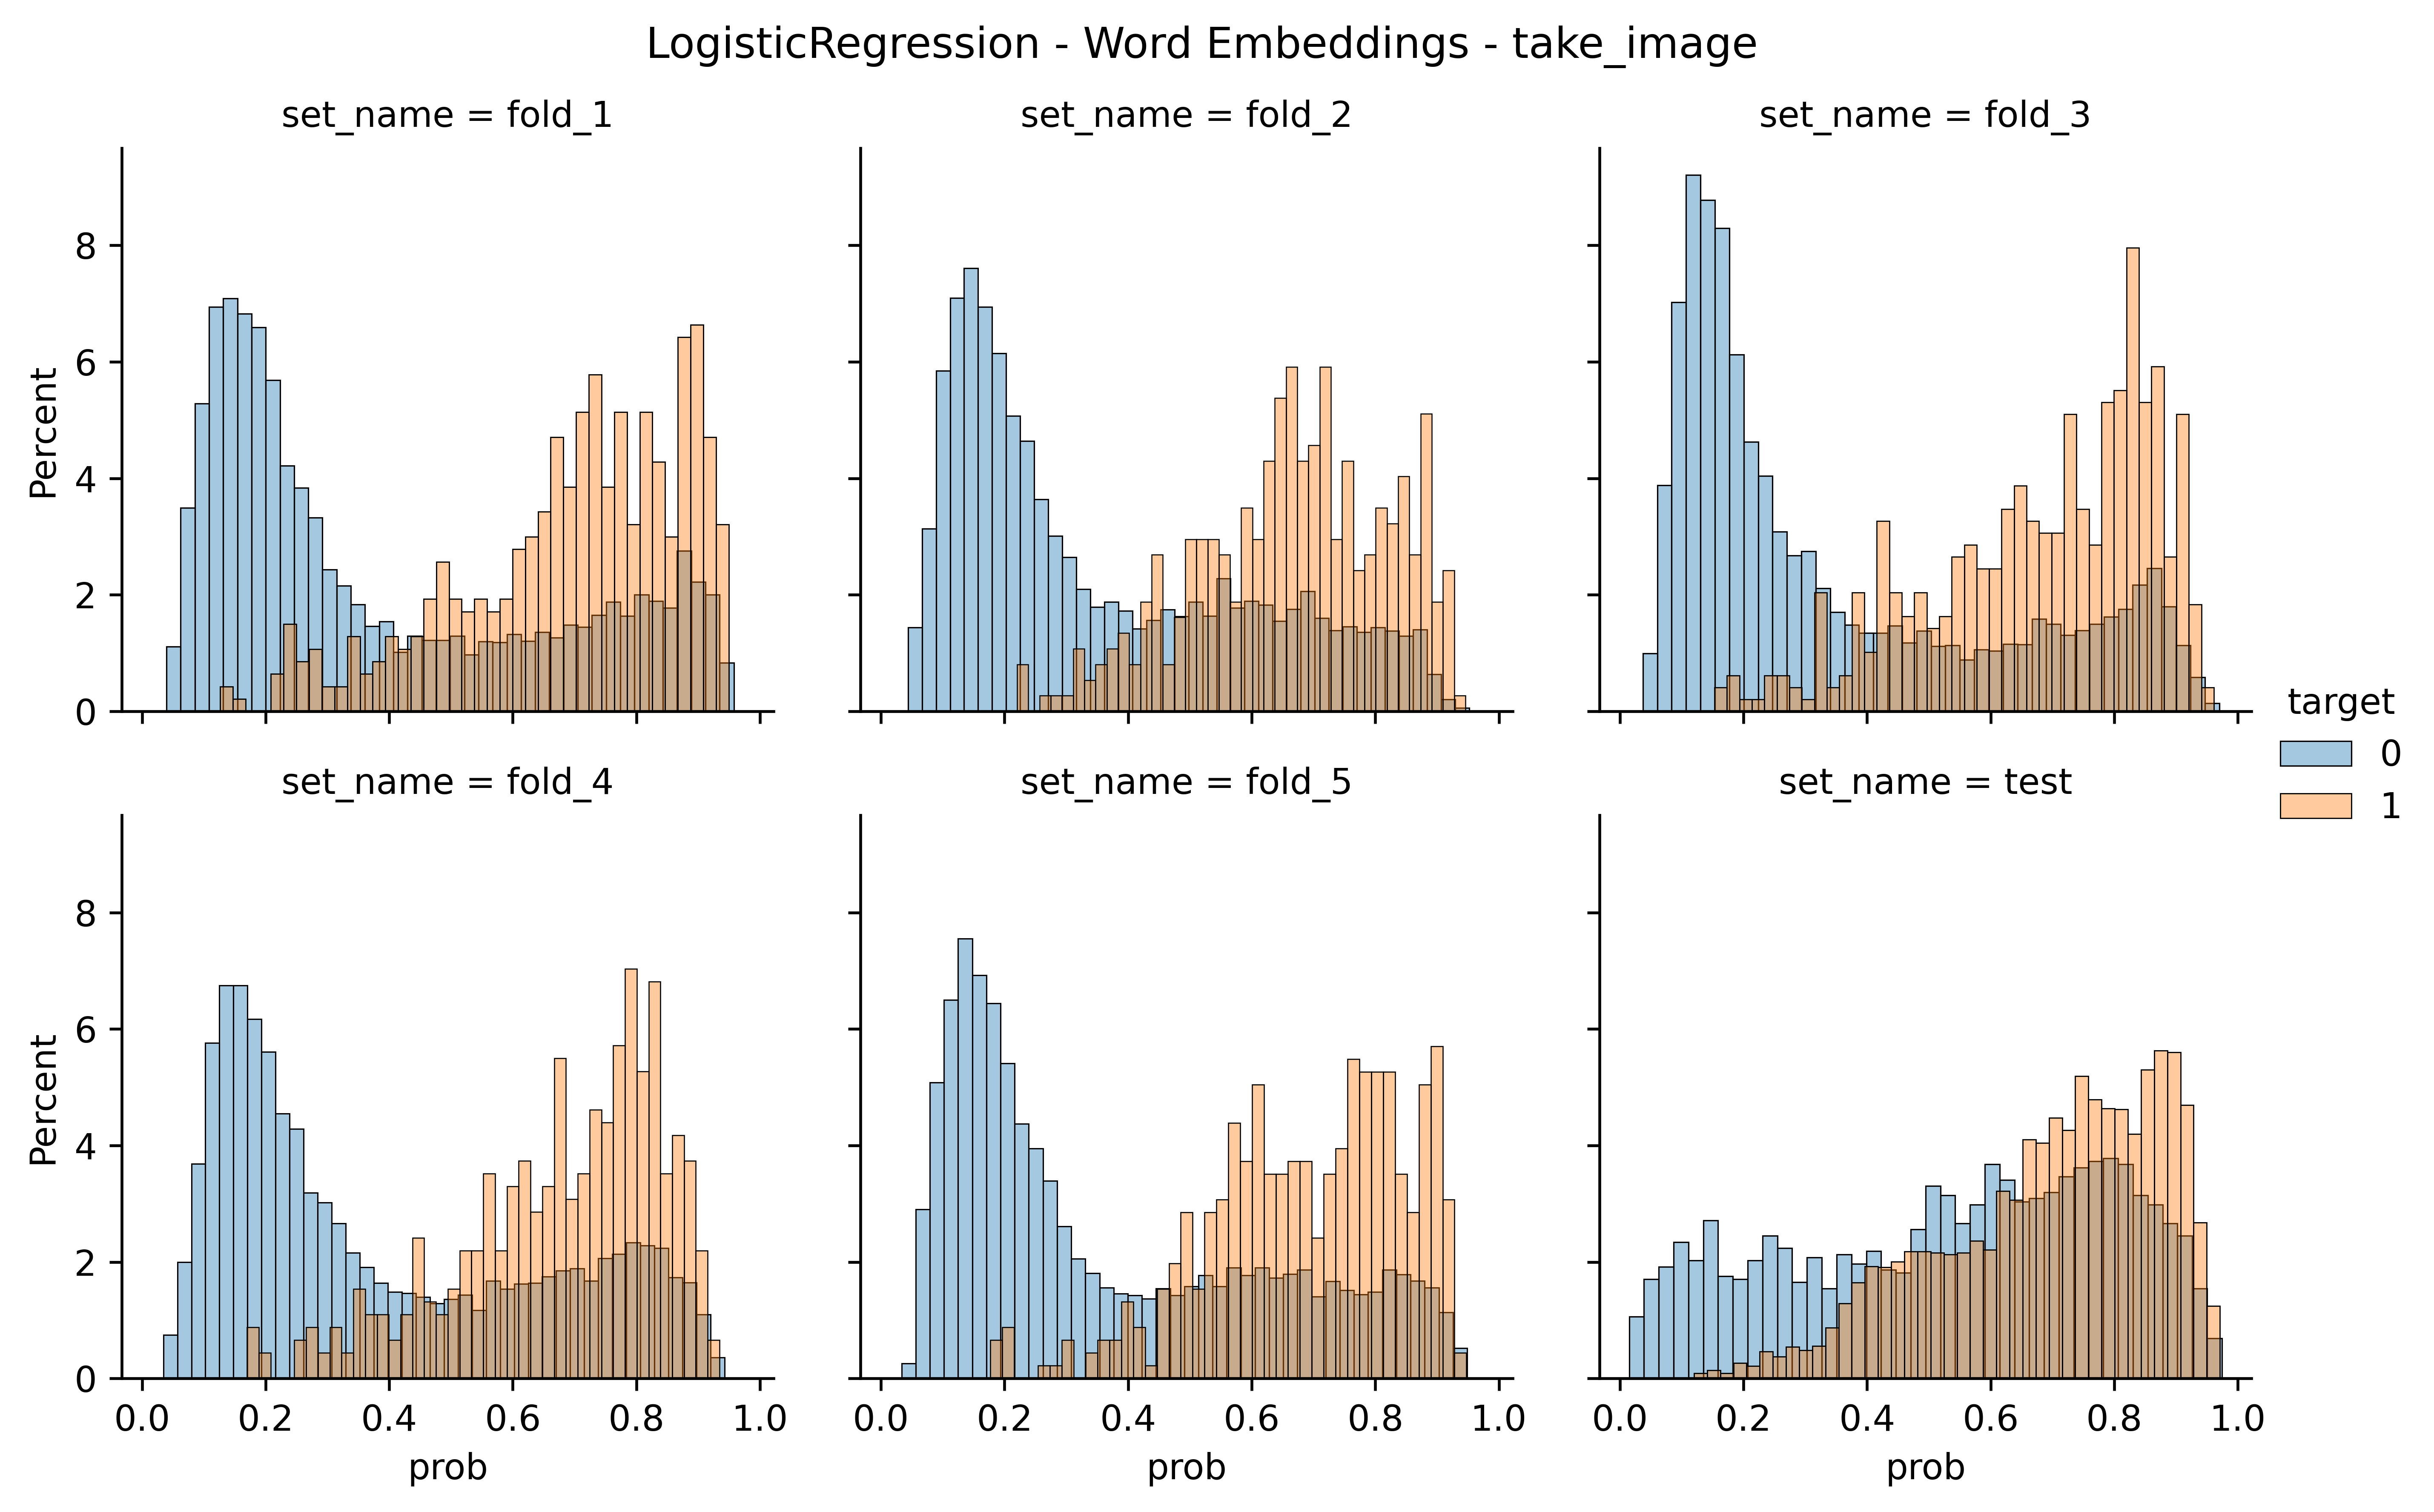
\includegraphics[width=\linewidth]{figures/results/word_embeddings/lgr/take_image/lgr__distplot.png}
        \caption{Distribución de predicciones en validación cruzada y el conjunto de test.}
        \label{fig:my_label}
    \end{subfigure}
    \hfill
    \begin{subfigure}[b]{\textwidth}
    \minipage{0.32\textwidth}
      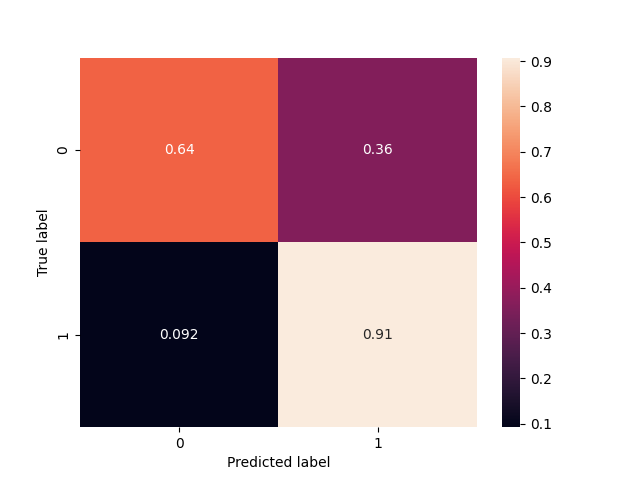
\includegraphics[width=\linewidth]{figures/results/word_embeddings/lgr/take_image/lgr_set_1_confusion_matrix_percent.png}
    \endminipage\hfill
    \minipage{0.32\textwidth}
      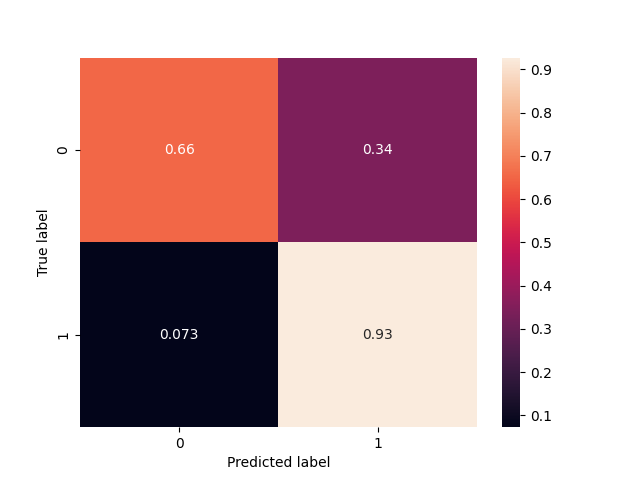
\includegraphics[width=\linewidth]{figures/results/word_embeddings/lgr/take_image/lgr_set_2_confusion_matrix_percent.png}
    \endminipage\hfill
    \minipage{0.32\textwidth}%
      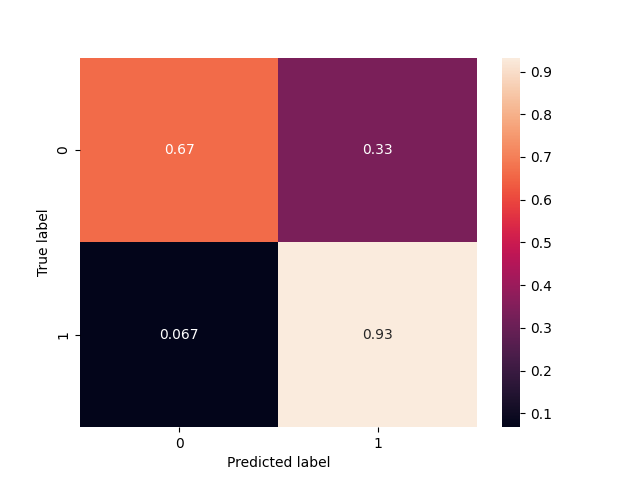
\includegraphics[width=\linewidth]{figures/results/word_embeddings/lgr/take_image/lgr_set_3_confusion_matrix_percent.png}
    \endminipage
    
    \medskip
    
    \minipage{0.32\textwidth}
      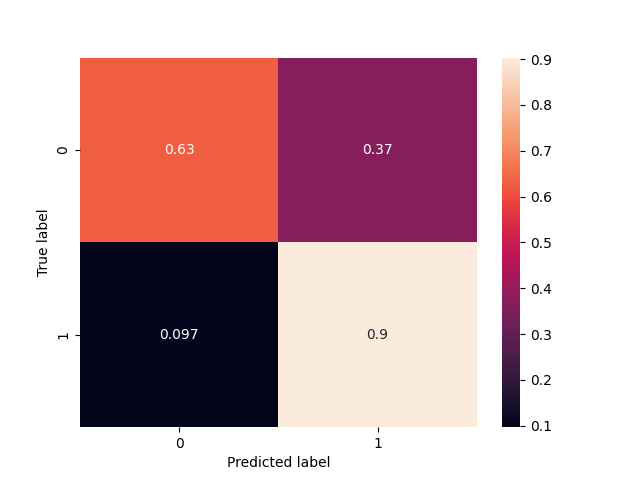
\includegraphics[width=\linewidth]{figures/results/word_embeddings/lgr/take_image/lgr_set_4_confusion_matrix_percent.png}
    \endminipage\hfill
    \minipage{0.32\textwidth}
      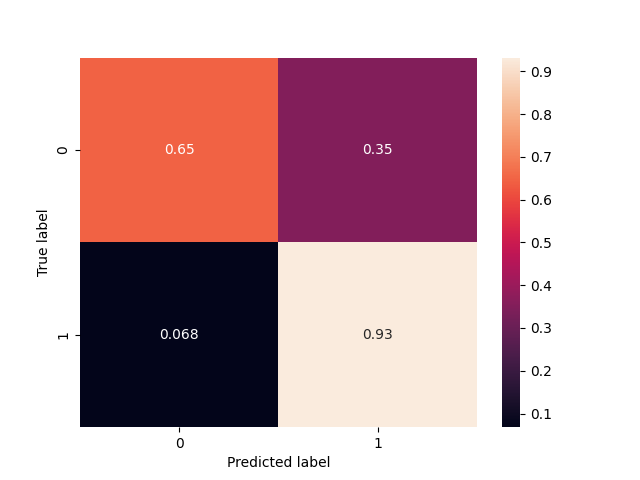
\includegraphics[width=\linewidth]{figures/results/word_embeddings/lgr/take_image/lgr_set_5_confusion_matrix_percent.png}
    \endminipage\hfill
    \minipage{0.32\textwidth}%
      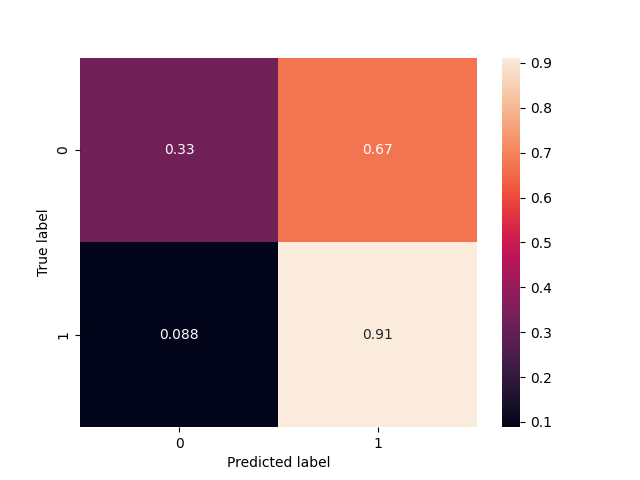
\includegraphics[width=\linewidth]{figures/results/word_embeddings/lgr/take_image/lgr_set_6_confusion_matrix_percent.png}
    \endminipage
    \caption{Matrices de confusión en validación cruzada y el conjunto de test}
    \end{subfigure}
    \caption{Resultados del modelo de regresión logística con codificación por word embeddings y esquema de acción take\_image.}
\end{figure}


\begin{figure}
    \centering
    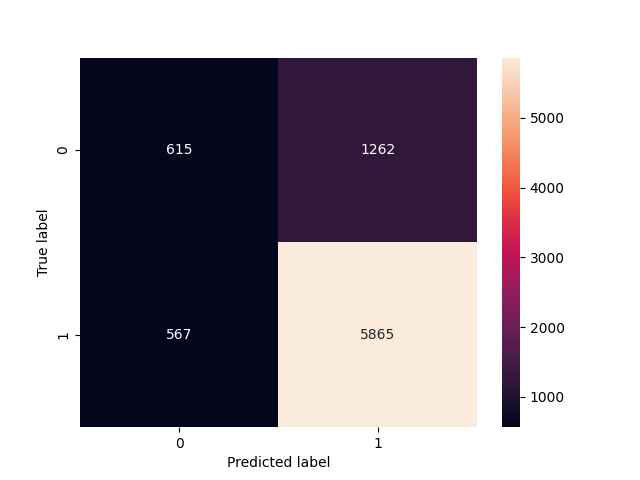
\includegraphics[scale=0.7]{figures/results/word_embeddings/lgr/take_image/lgr_set_6_confusion_matrix_raw.png}
    \caption{Matriz de confusión sin porcentajes del modelo de regresión logística con codificación por word embeddings y esquema de acción take\_image.}
    \label{fig:my_label}
\end{figure}

\begin{table}[h!]
\centering
\scalebox{0.9}{
 \begin{tabular}{|c || c | c | c | c | c | c |} 
 \hline
  Esquemas & Precisión & Recall & $H_{1.5}$ & $F_{1.5}$ & Umbral de decisión & Modelo \\
 \hline
 take\_image & 0.8088 & 0.997 & 0.4351 & 0.997 & 0.61 & LGR \\
 calibrate & 0.0467 & 0.4743 & 0.5083 & 0.1242 & 0.728 & NN\\
 switch\_on  & 0.0405 & 0.4567 & 0.5106 & 0.1097 & 0.576 & NN\\
 switch\_off & 0.0476 & 0.1818 & 0.2422 & 0.0876 & 0.034 & NN \\
 turn\_to  & - & - & - & - & - & -\\[1ex]
 \hline
 \end{tabular}}
 \caption{Resultados por esquema de acción del mejor modelo con codificación por word embeddings.}
 \label{results:ad-hoc-calibrate}
\end{table}


\section{Modelos predictivos ad-hoc}
\label{exp:wb}

\subsection{Configuración del experimento}

Como contraparte del experimento anterior, usaremos la codificación por word embeddings, bajo el mismo conjunto de entrenamientos y construcción de ventanas, con la salvedad de ser codificados a partir del modelo de lenguaje de FastText, entrenado con oraciones provenientes de planes relajados. El modelo de lenguaje es un modelo Skipgram entrenado por $100$ épocas, un tamaño de ventana de contexto de $3$ palabras, y un vector de salida de dimensión $30$. Se hicieron pruebas sobre otras configuraciones de parámetros pero el comportamiento que buscábamos que el modelo de lenguaje aprendiese ya era obtenido bajo esta configuración.

Los clasificadores y grillas de búsqueda de parámetros utilizadas fueron las mismos que los modelo predictivos ad-hoc.

\subsection{Resultados}

\begin{figure}
    \centering
    \begin{subfigure}[b]{0.83\textwidth}
    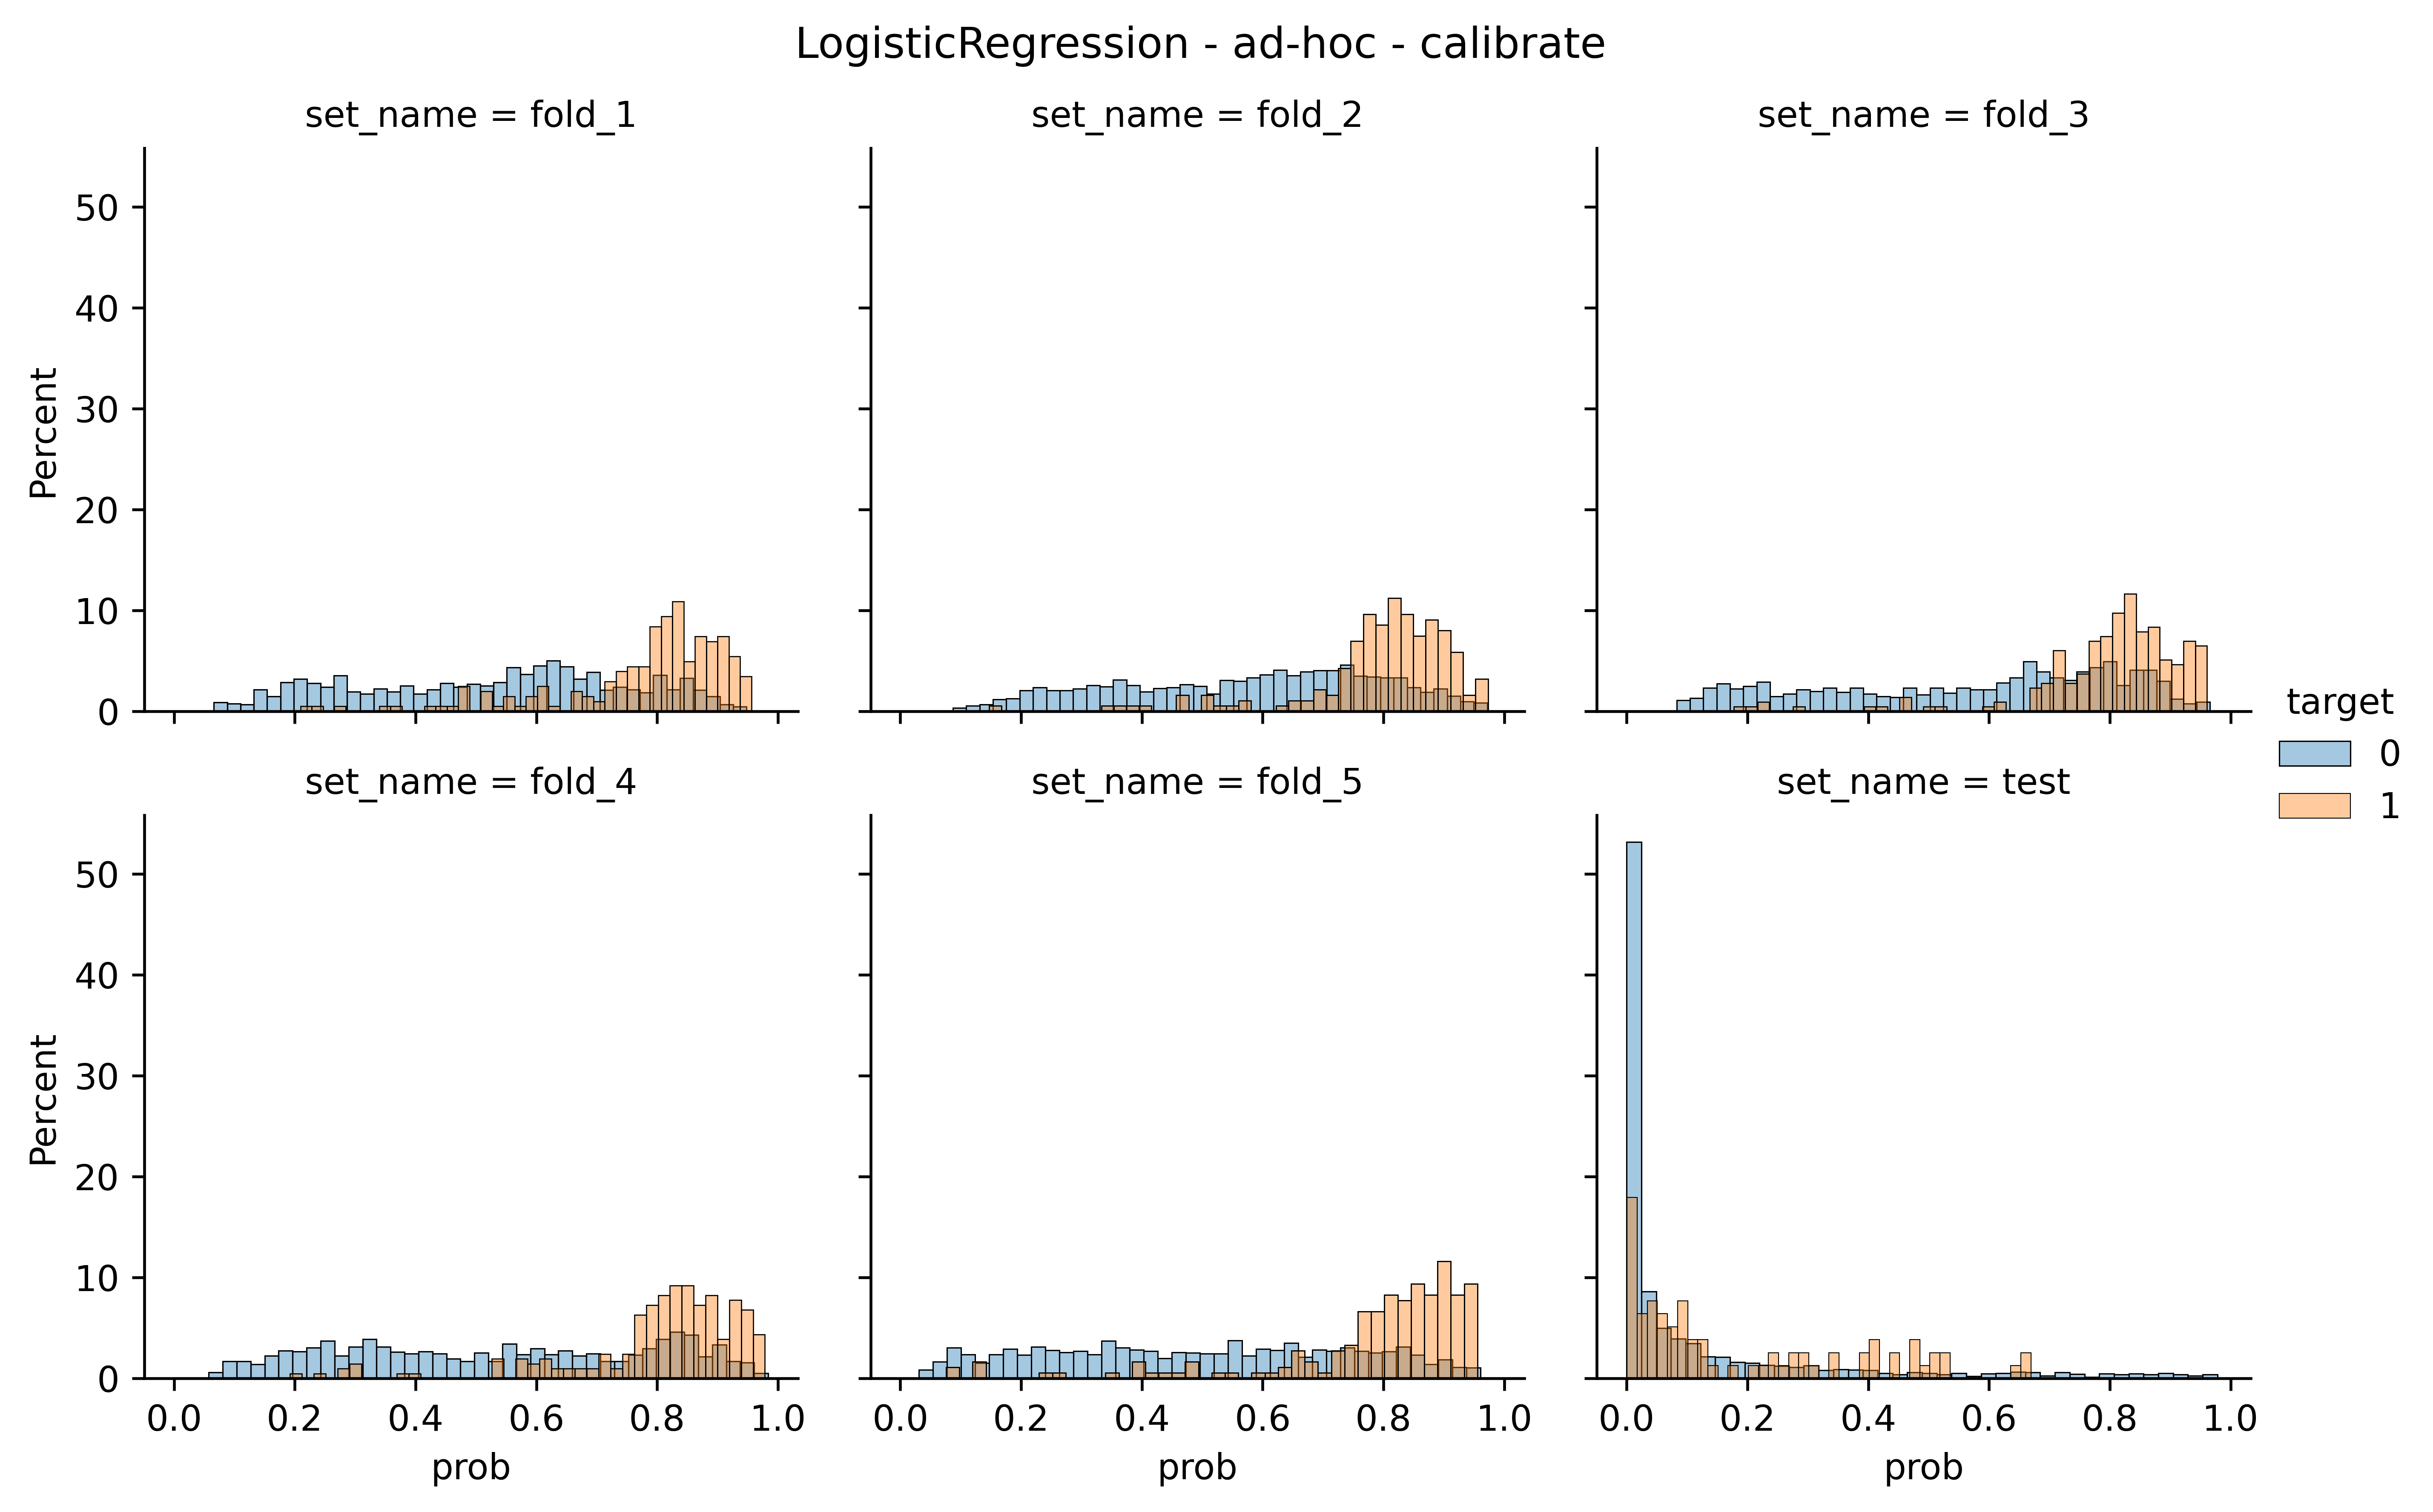
\includegraphics[width=\linewidth]{figures/results/ad-hoc/lgr/calibrate/calibrate__distplot.png}
    \end{subfigure}
    \hfill
    \centering
    \begin{subfigure}[b]{0.83\textwidth}
        \centering
        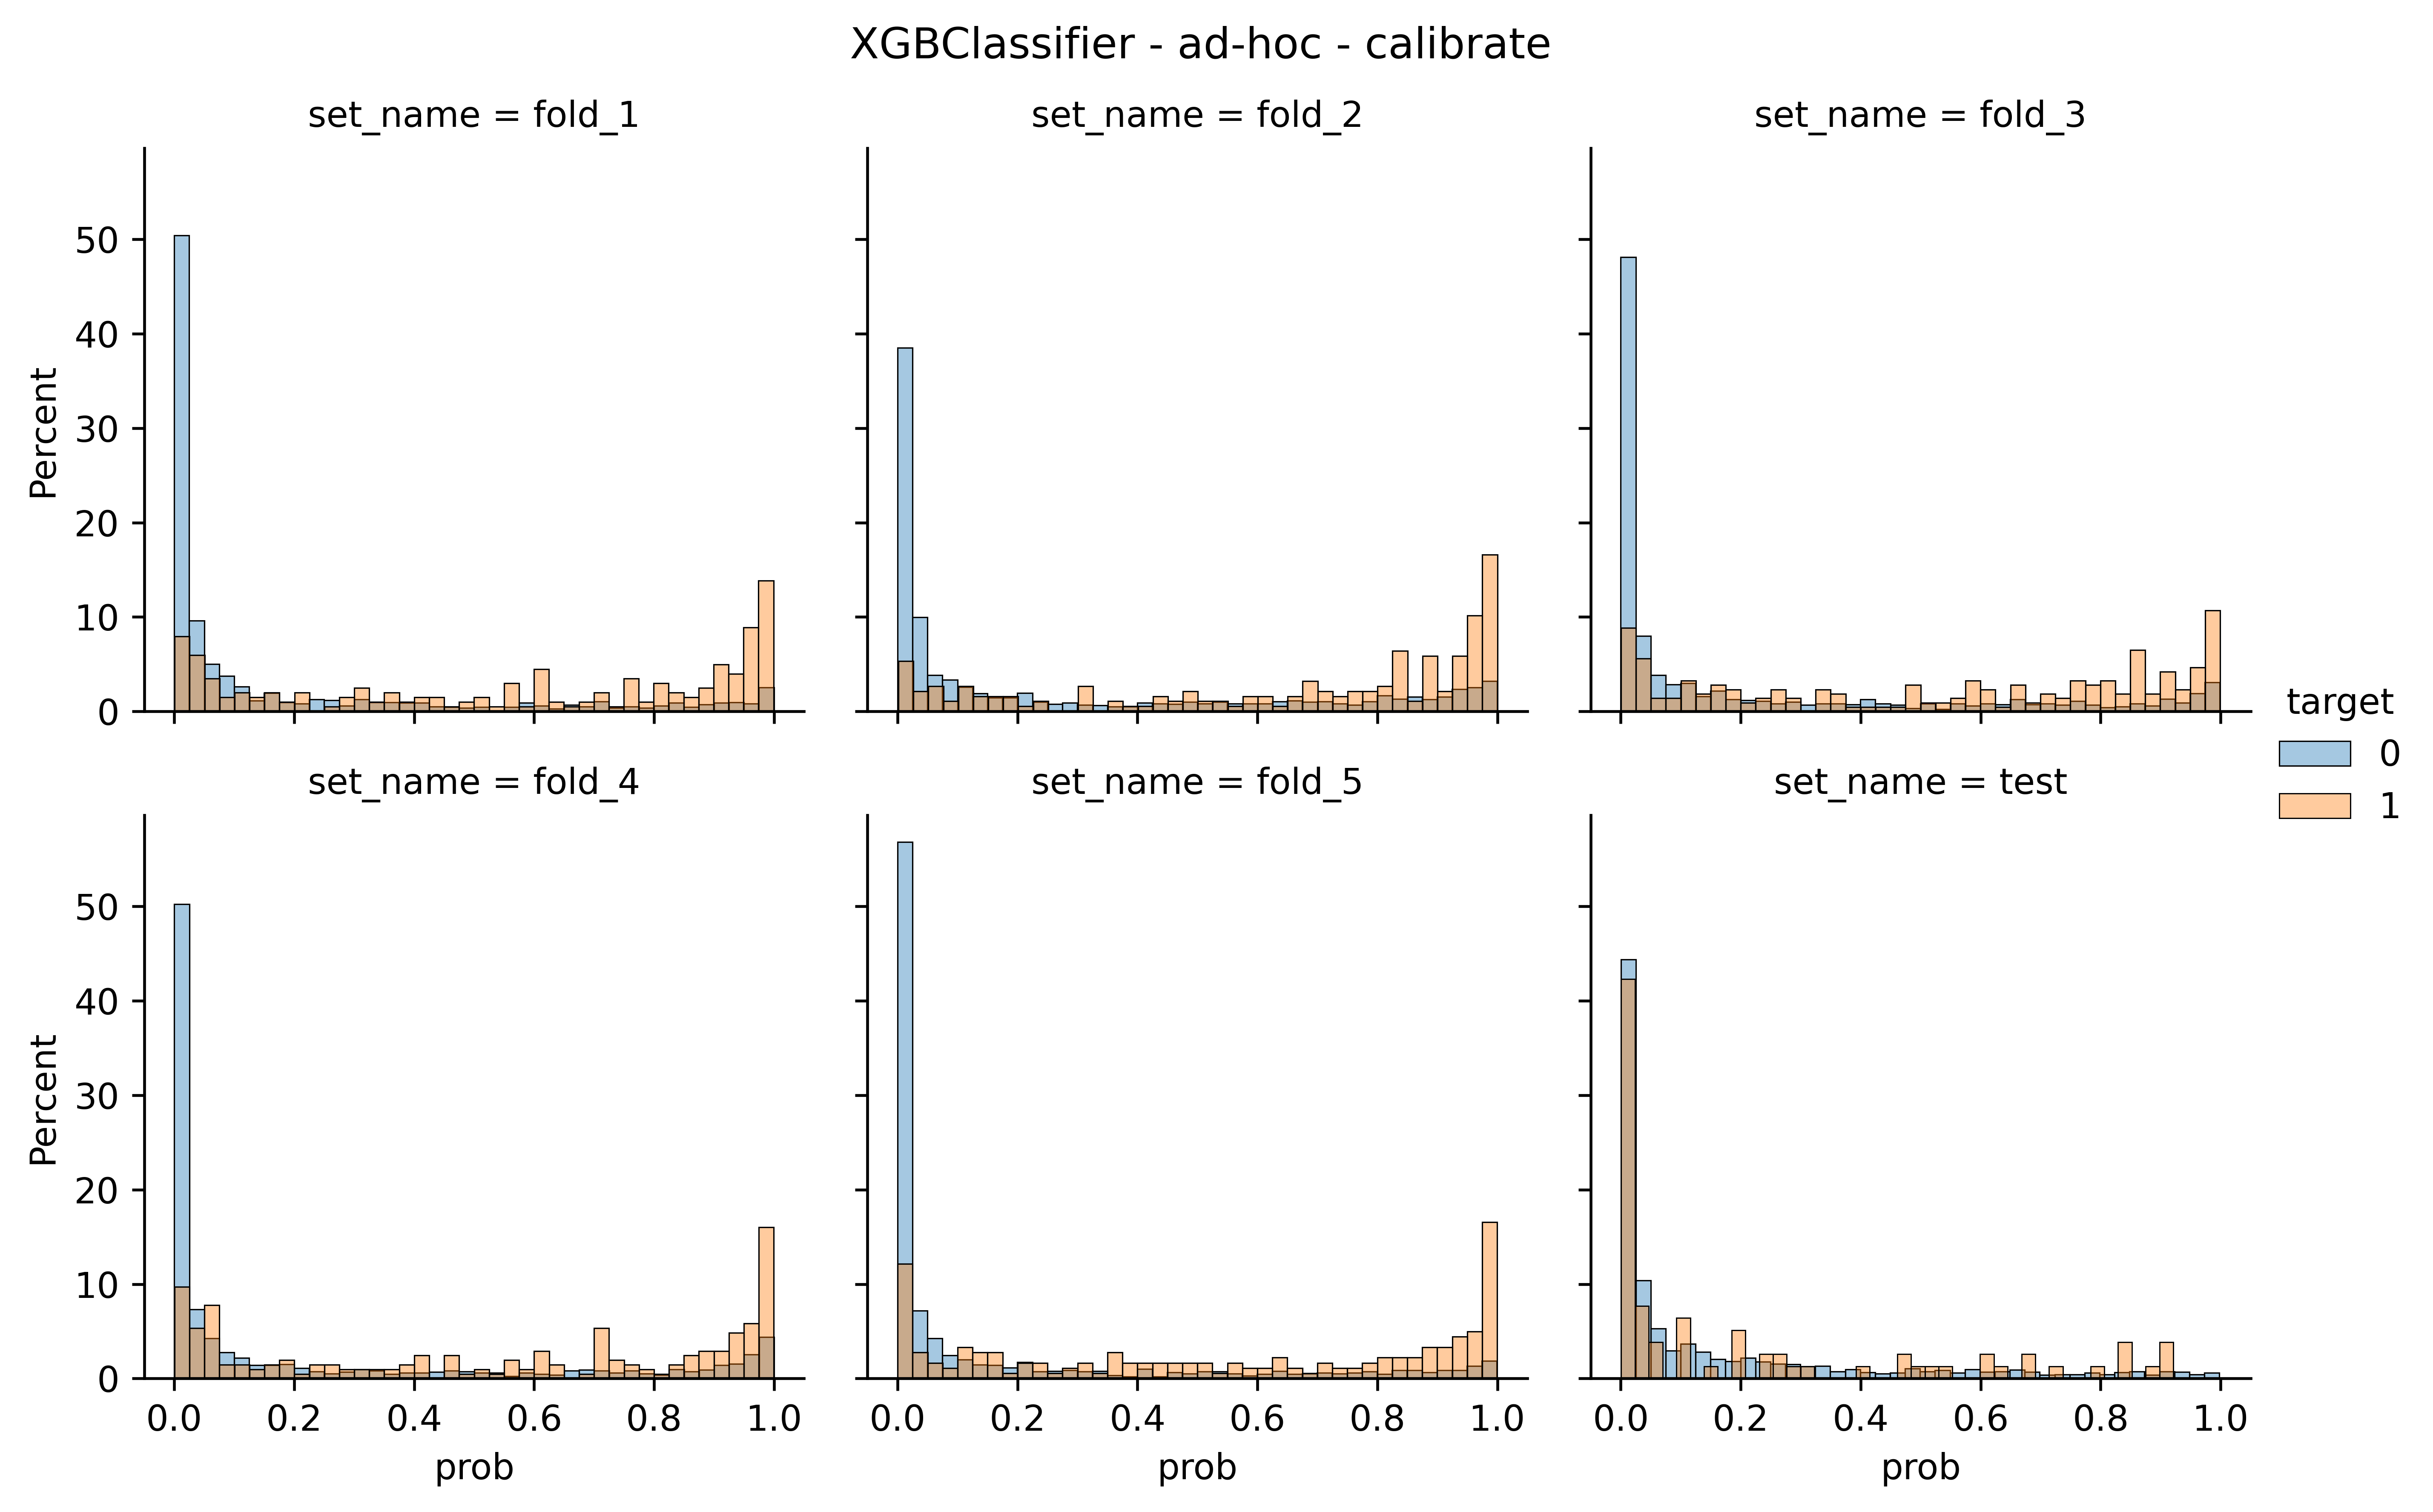
\includegraphics[width=\linewidth]{figures/results/ad-hoc/xgb/2021-12-07_06.29.19.600877__distplot (2).png}
    \end{subfigure}
    \hfill
    \centering
    \begin{subfigure}[b]{0.83\textwidth}
        \centering
        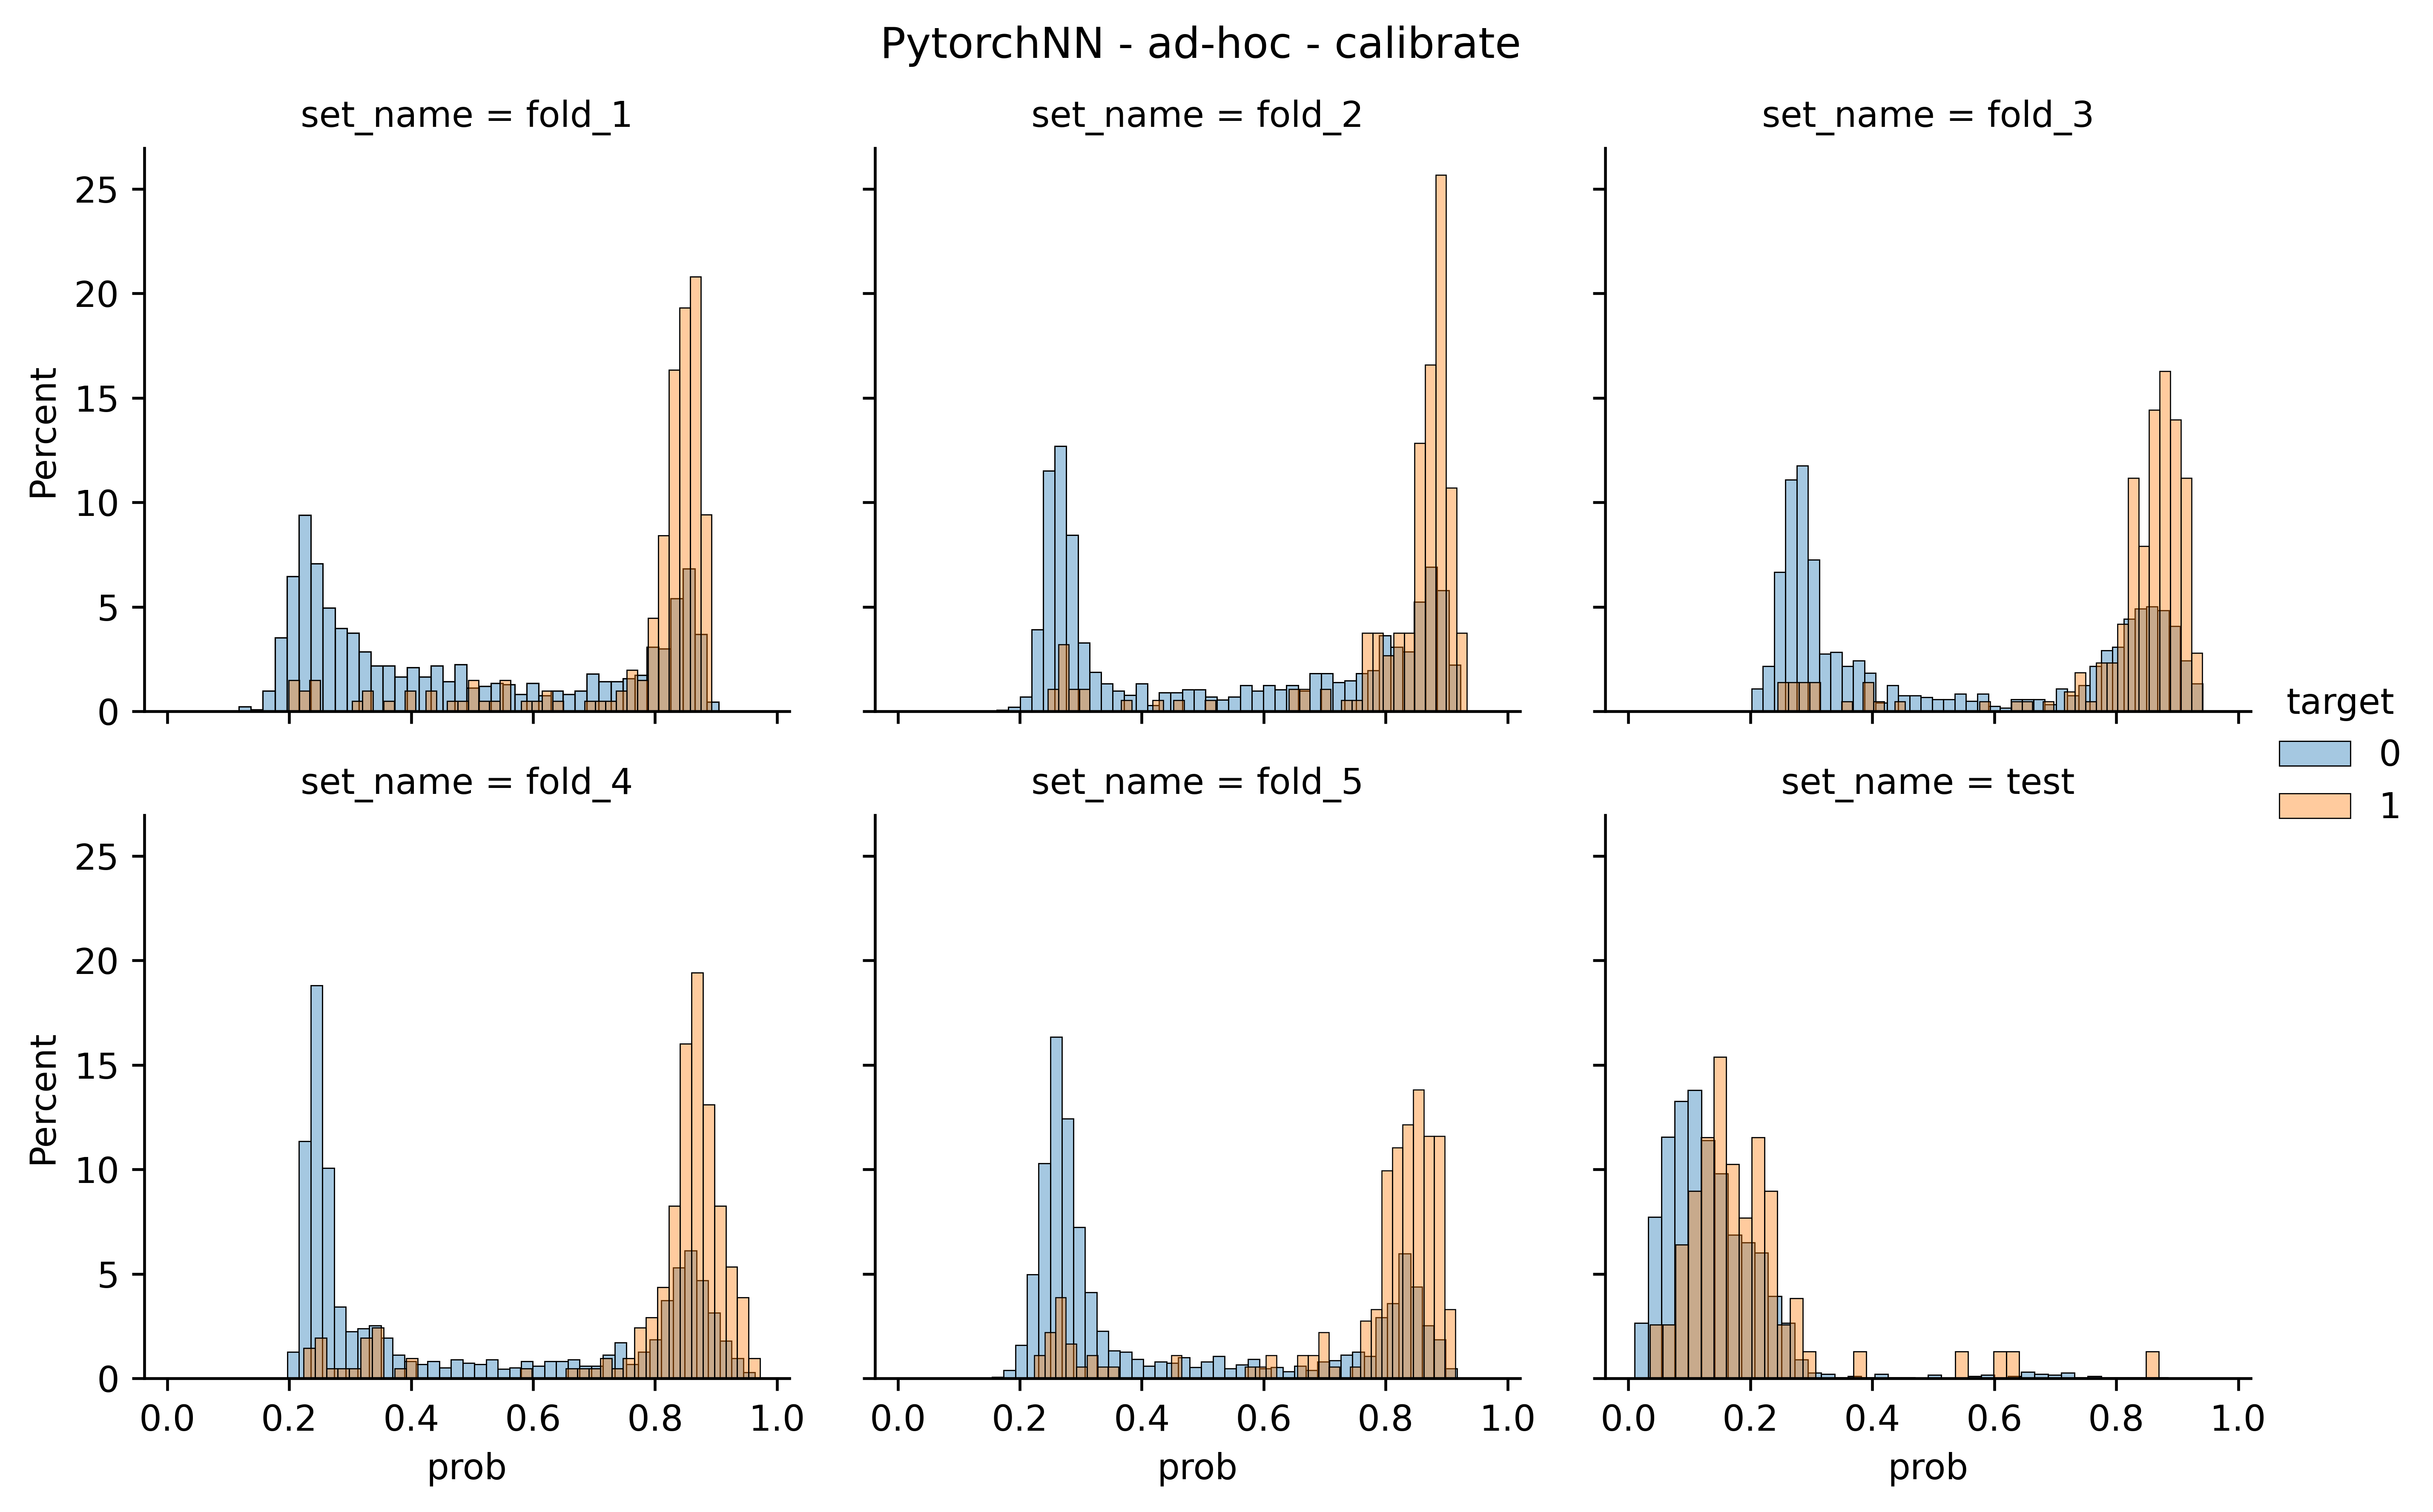
\includegraphics[width=\linewidth]{figures/results/ad-hoc/nn/2021-12-06_17.03.17.314982__distplot.png}
    \end{subfigure}
    \caption{Ad-hoc calibrate}
\end{figure}

\begin{figure}
    \centering
    \begin{subfigure}[b]{0.83\textwidth}
    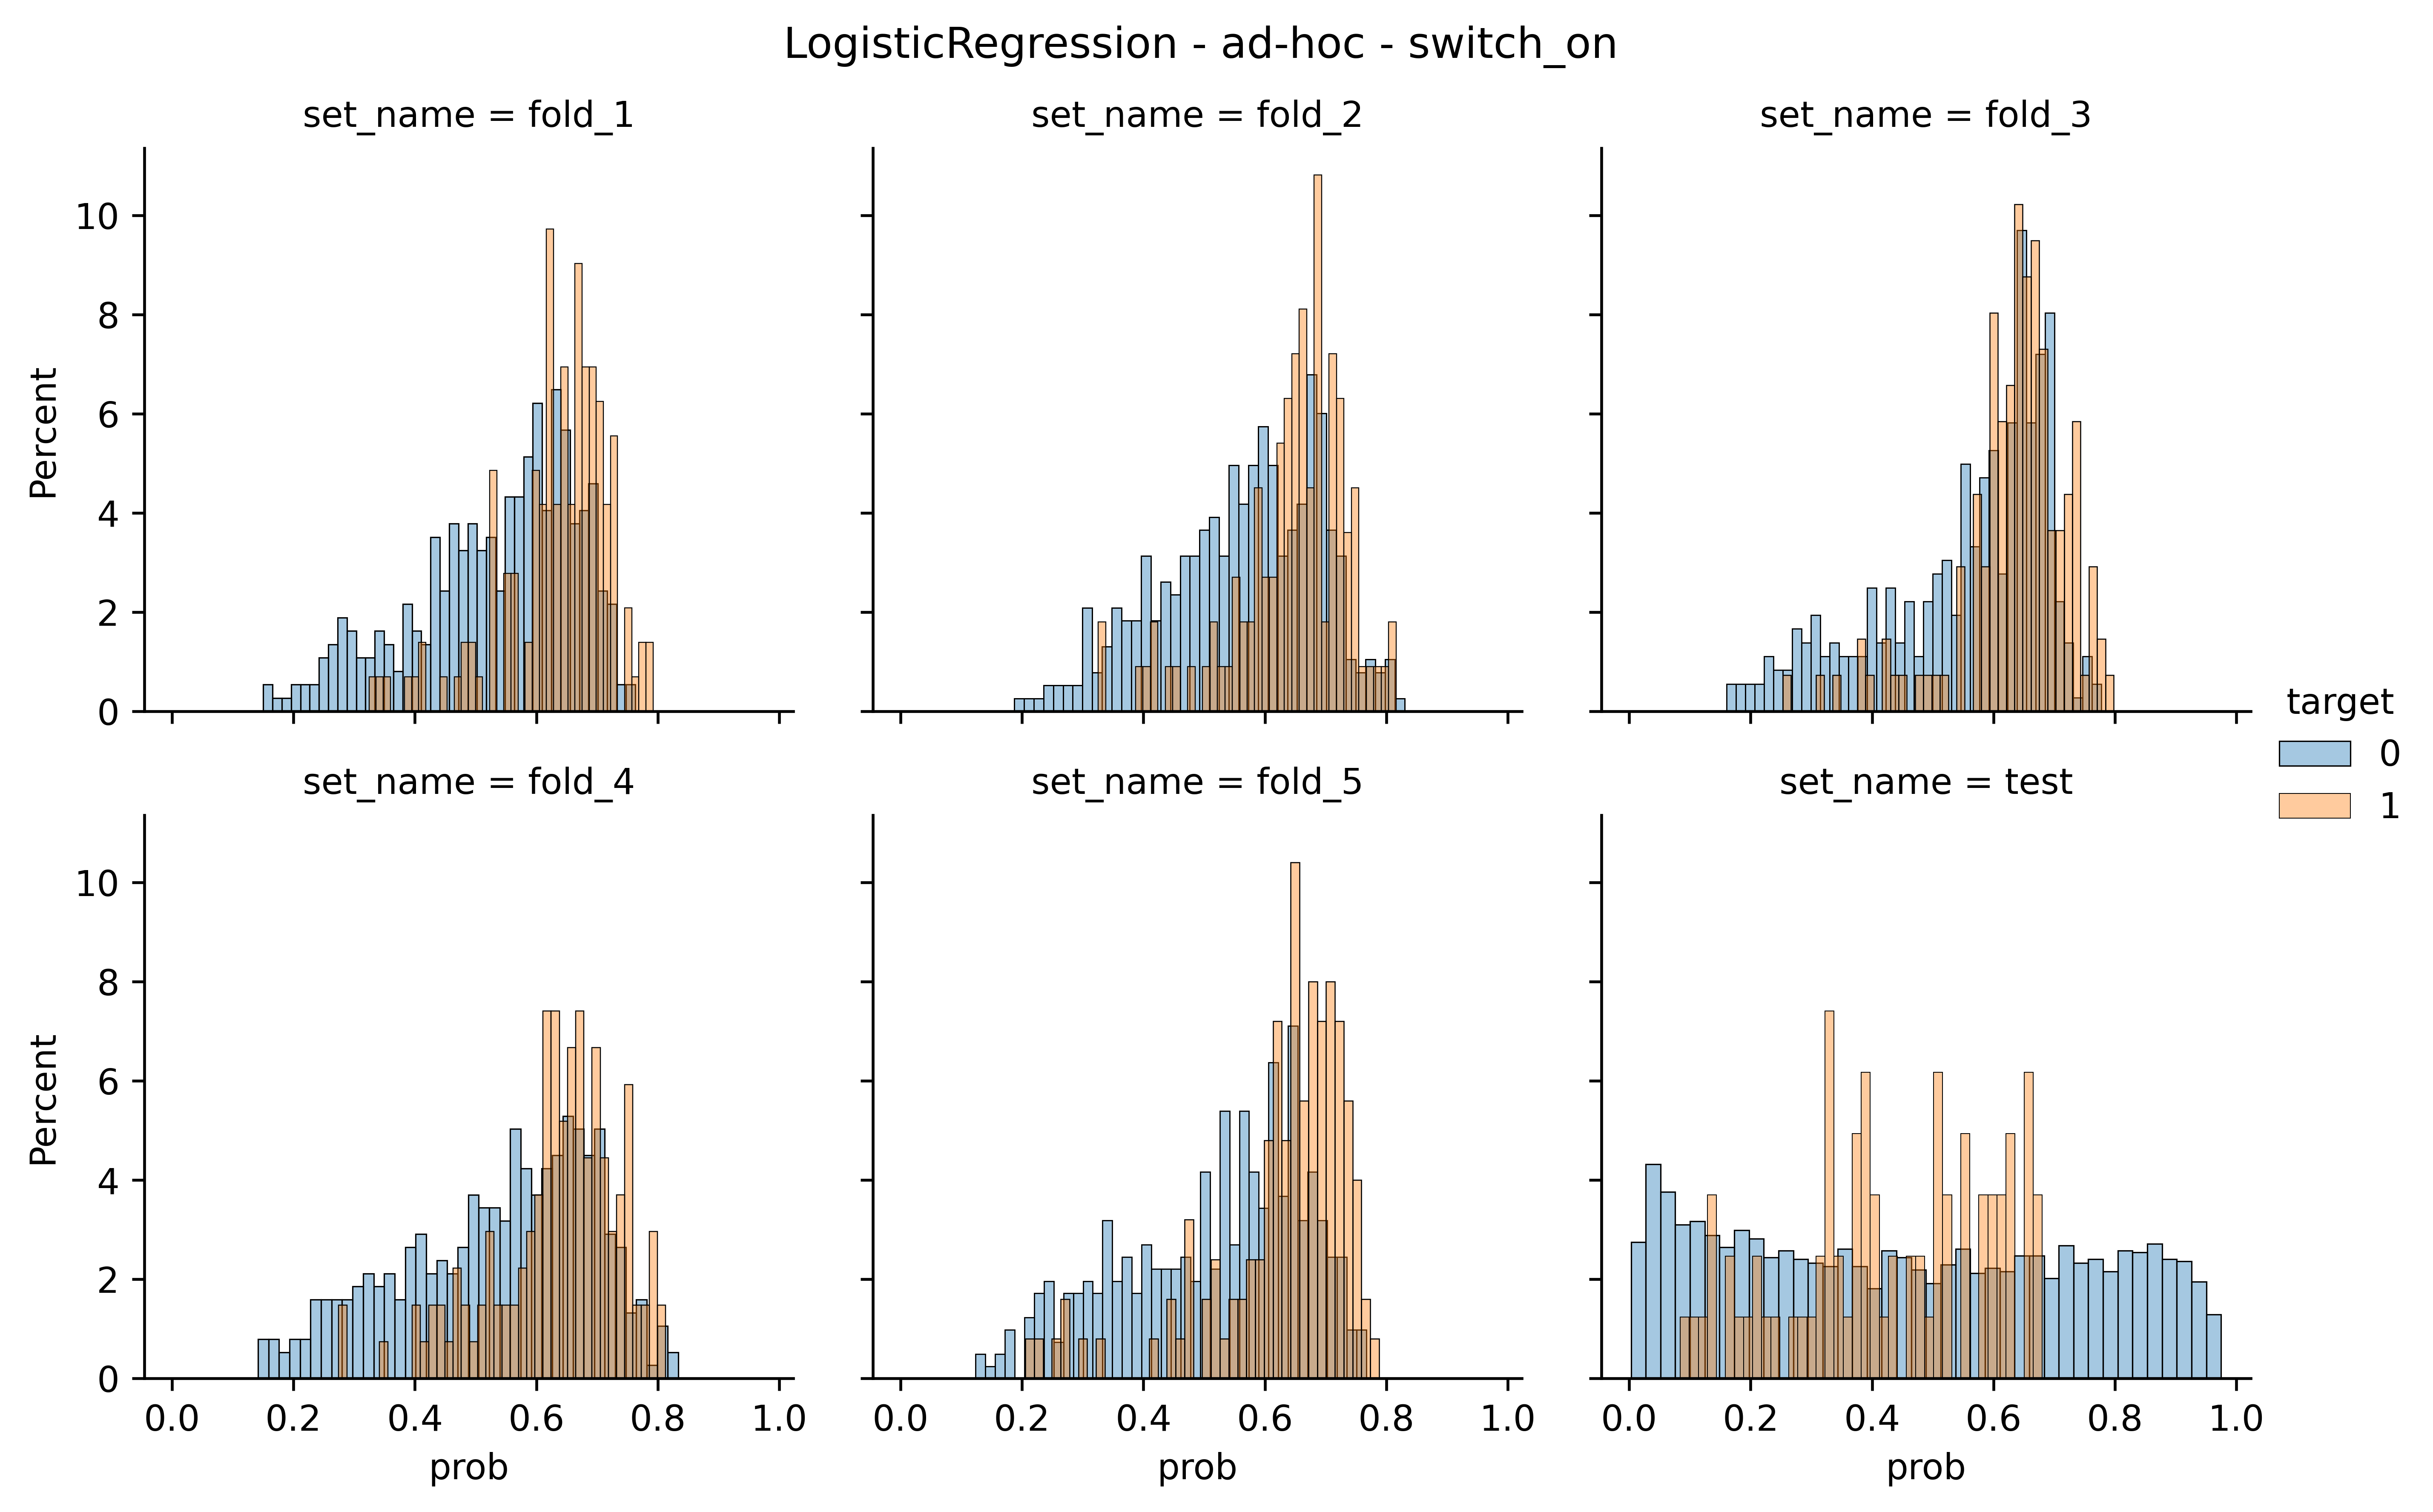
\includegraphics[width=\linewidth]{figures/results/ad-hoc/lgr/switch_on/turn_to__distplot.png}
    \end{subfigure}
    \hfill
    \centering
    \begin{subfigure}[b]{0.83\textwidth}
        \centering
        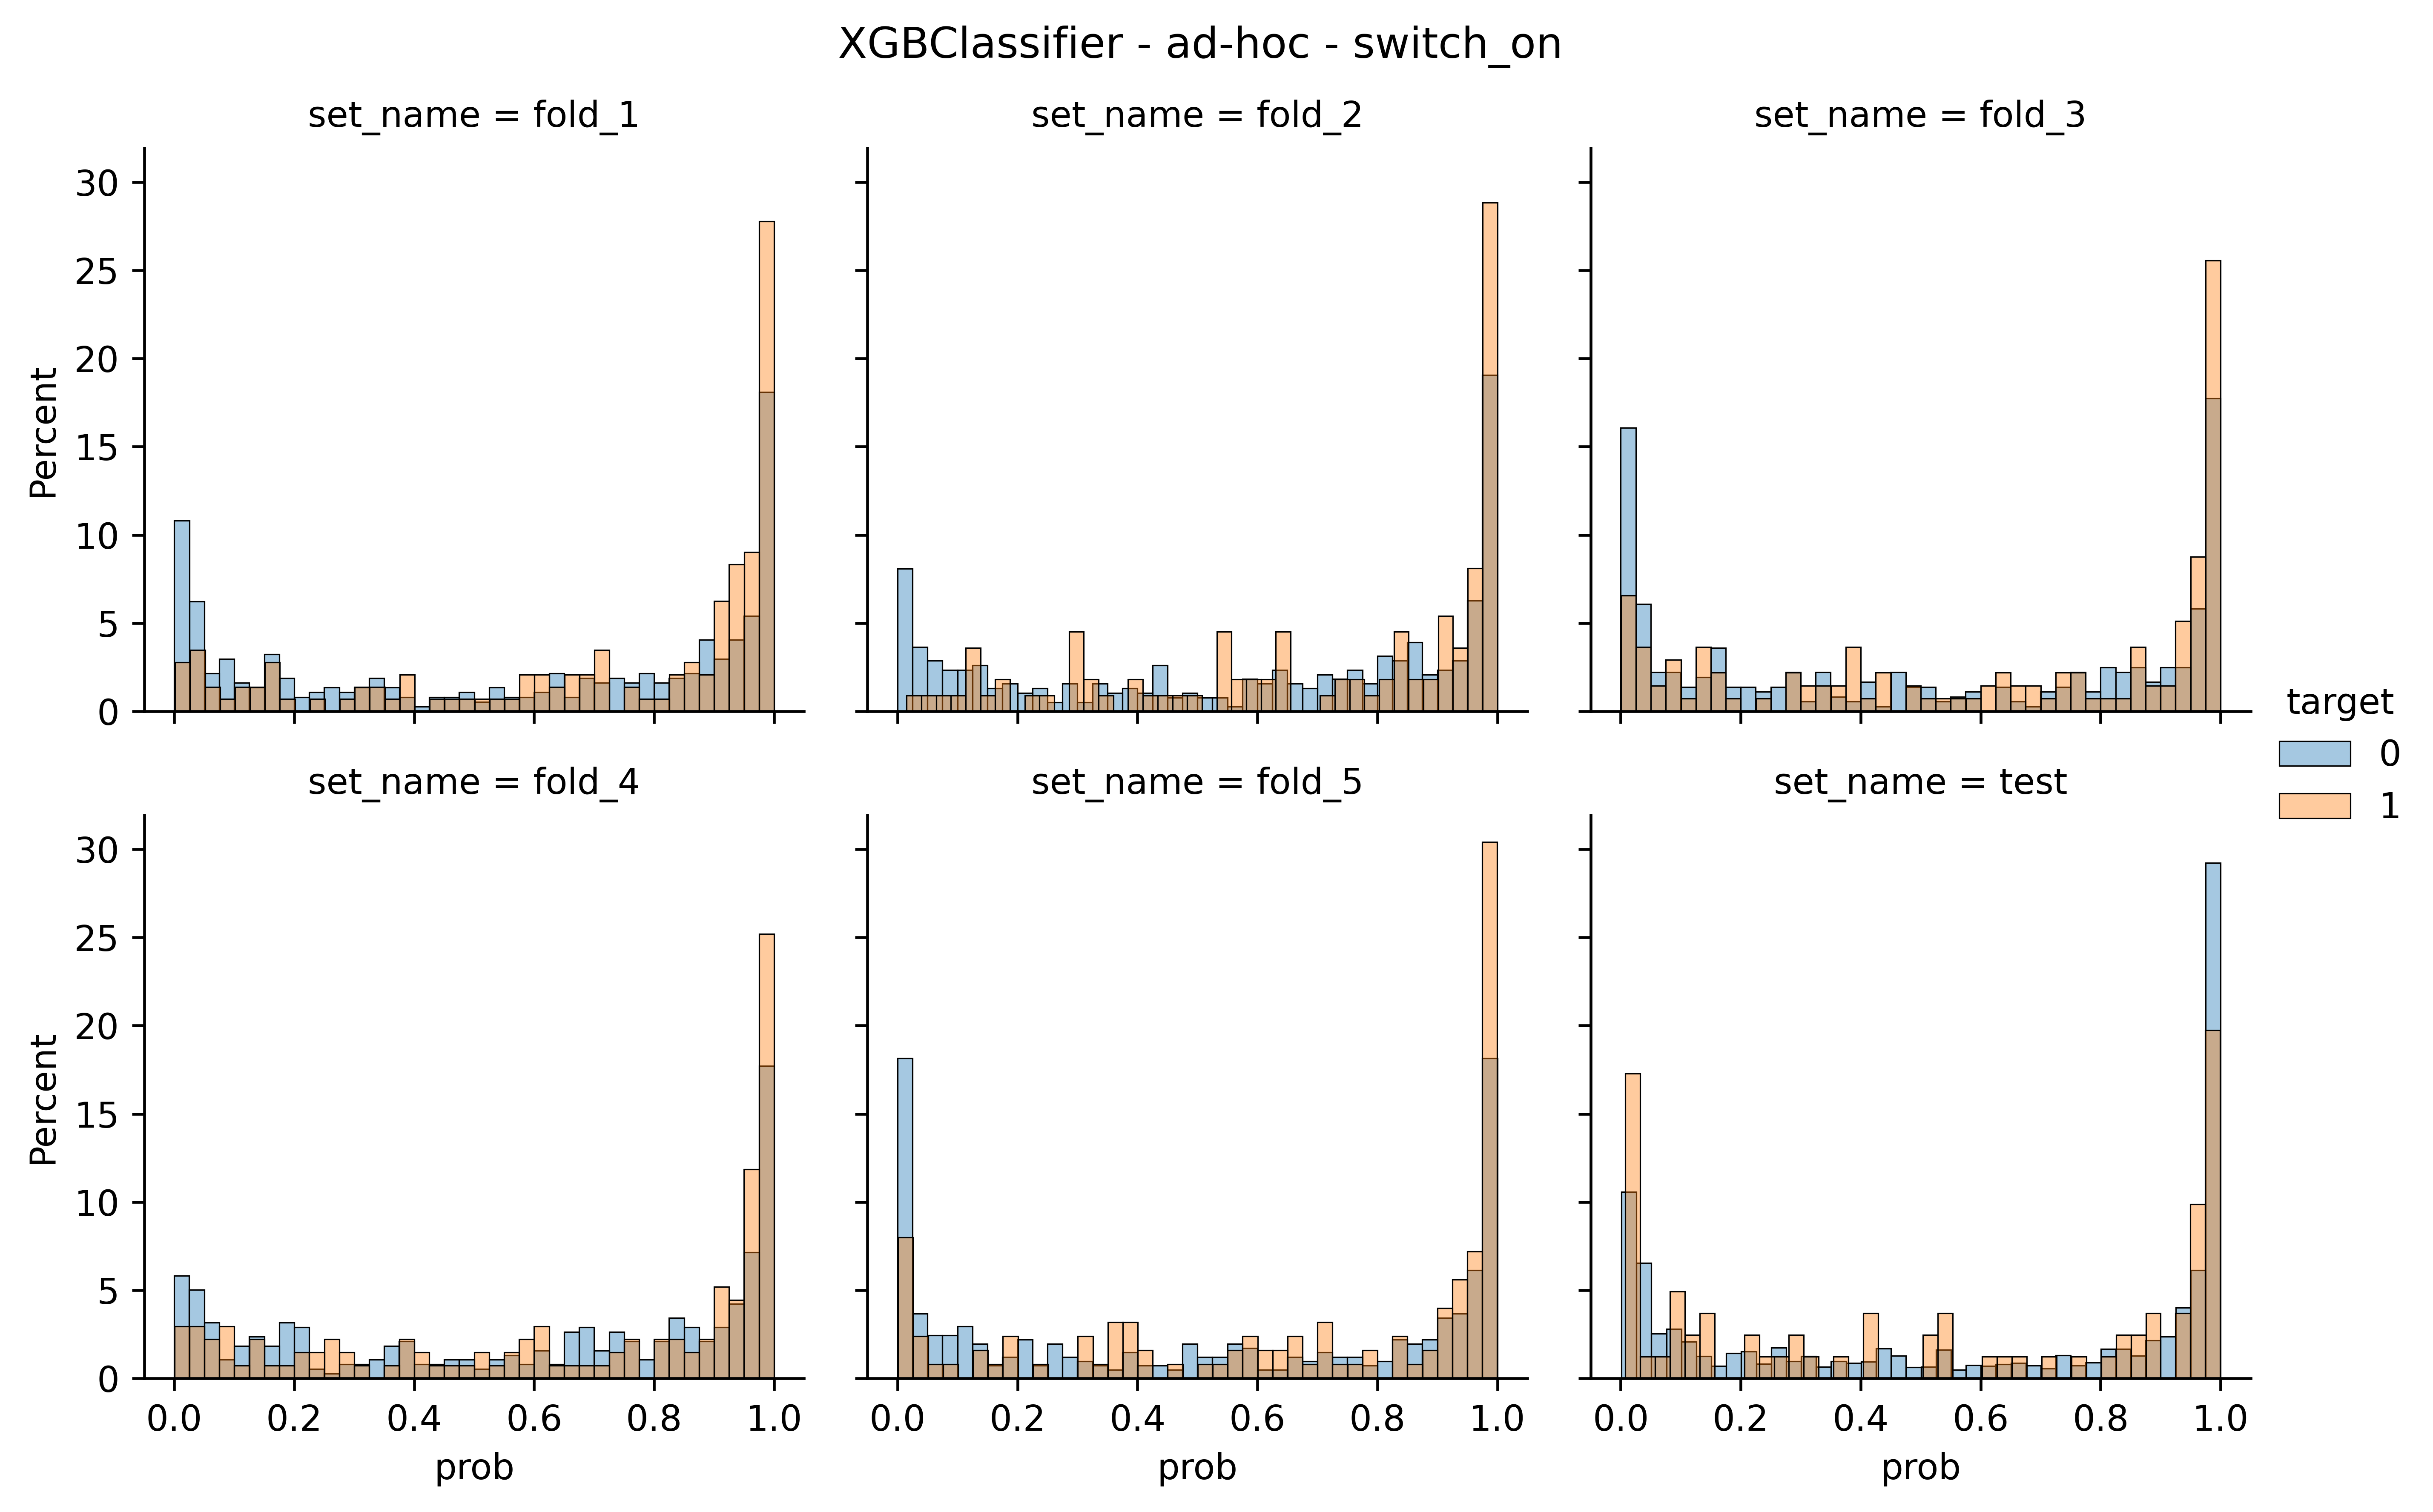
\includegraphics[width=\linewidth]{figures/results/ad-hoc/xgb/switch_on/2021-12-07_06.56.08.418411__distplot.png}
    \end{subfigure}
    \hfill
    \centering
    \begin{subfigure}[b]{0.83\textwidth}
        \centering
        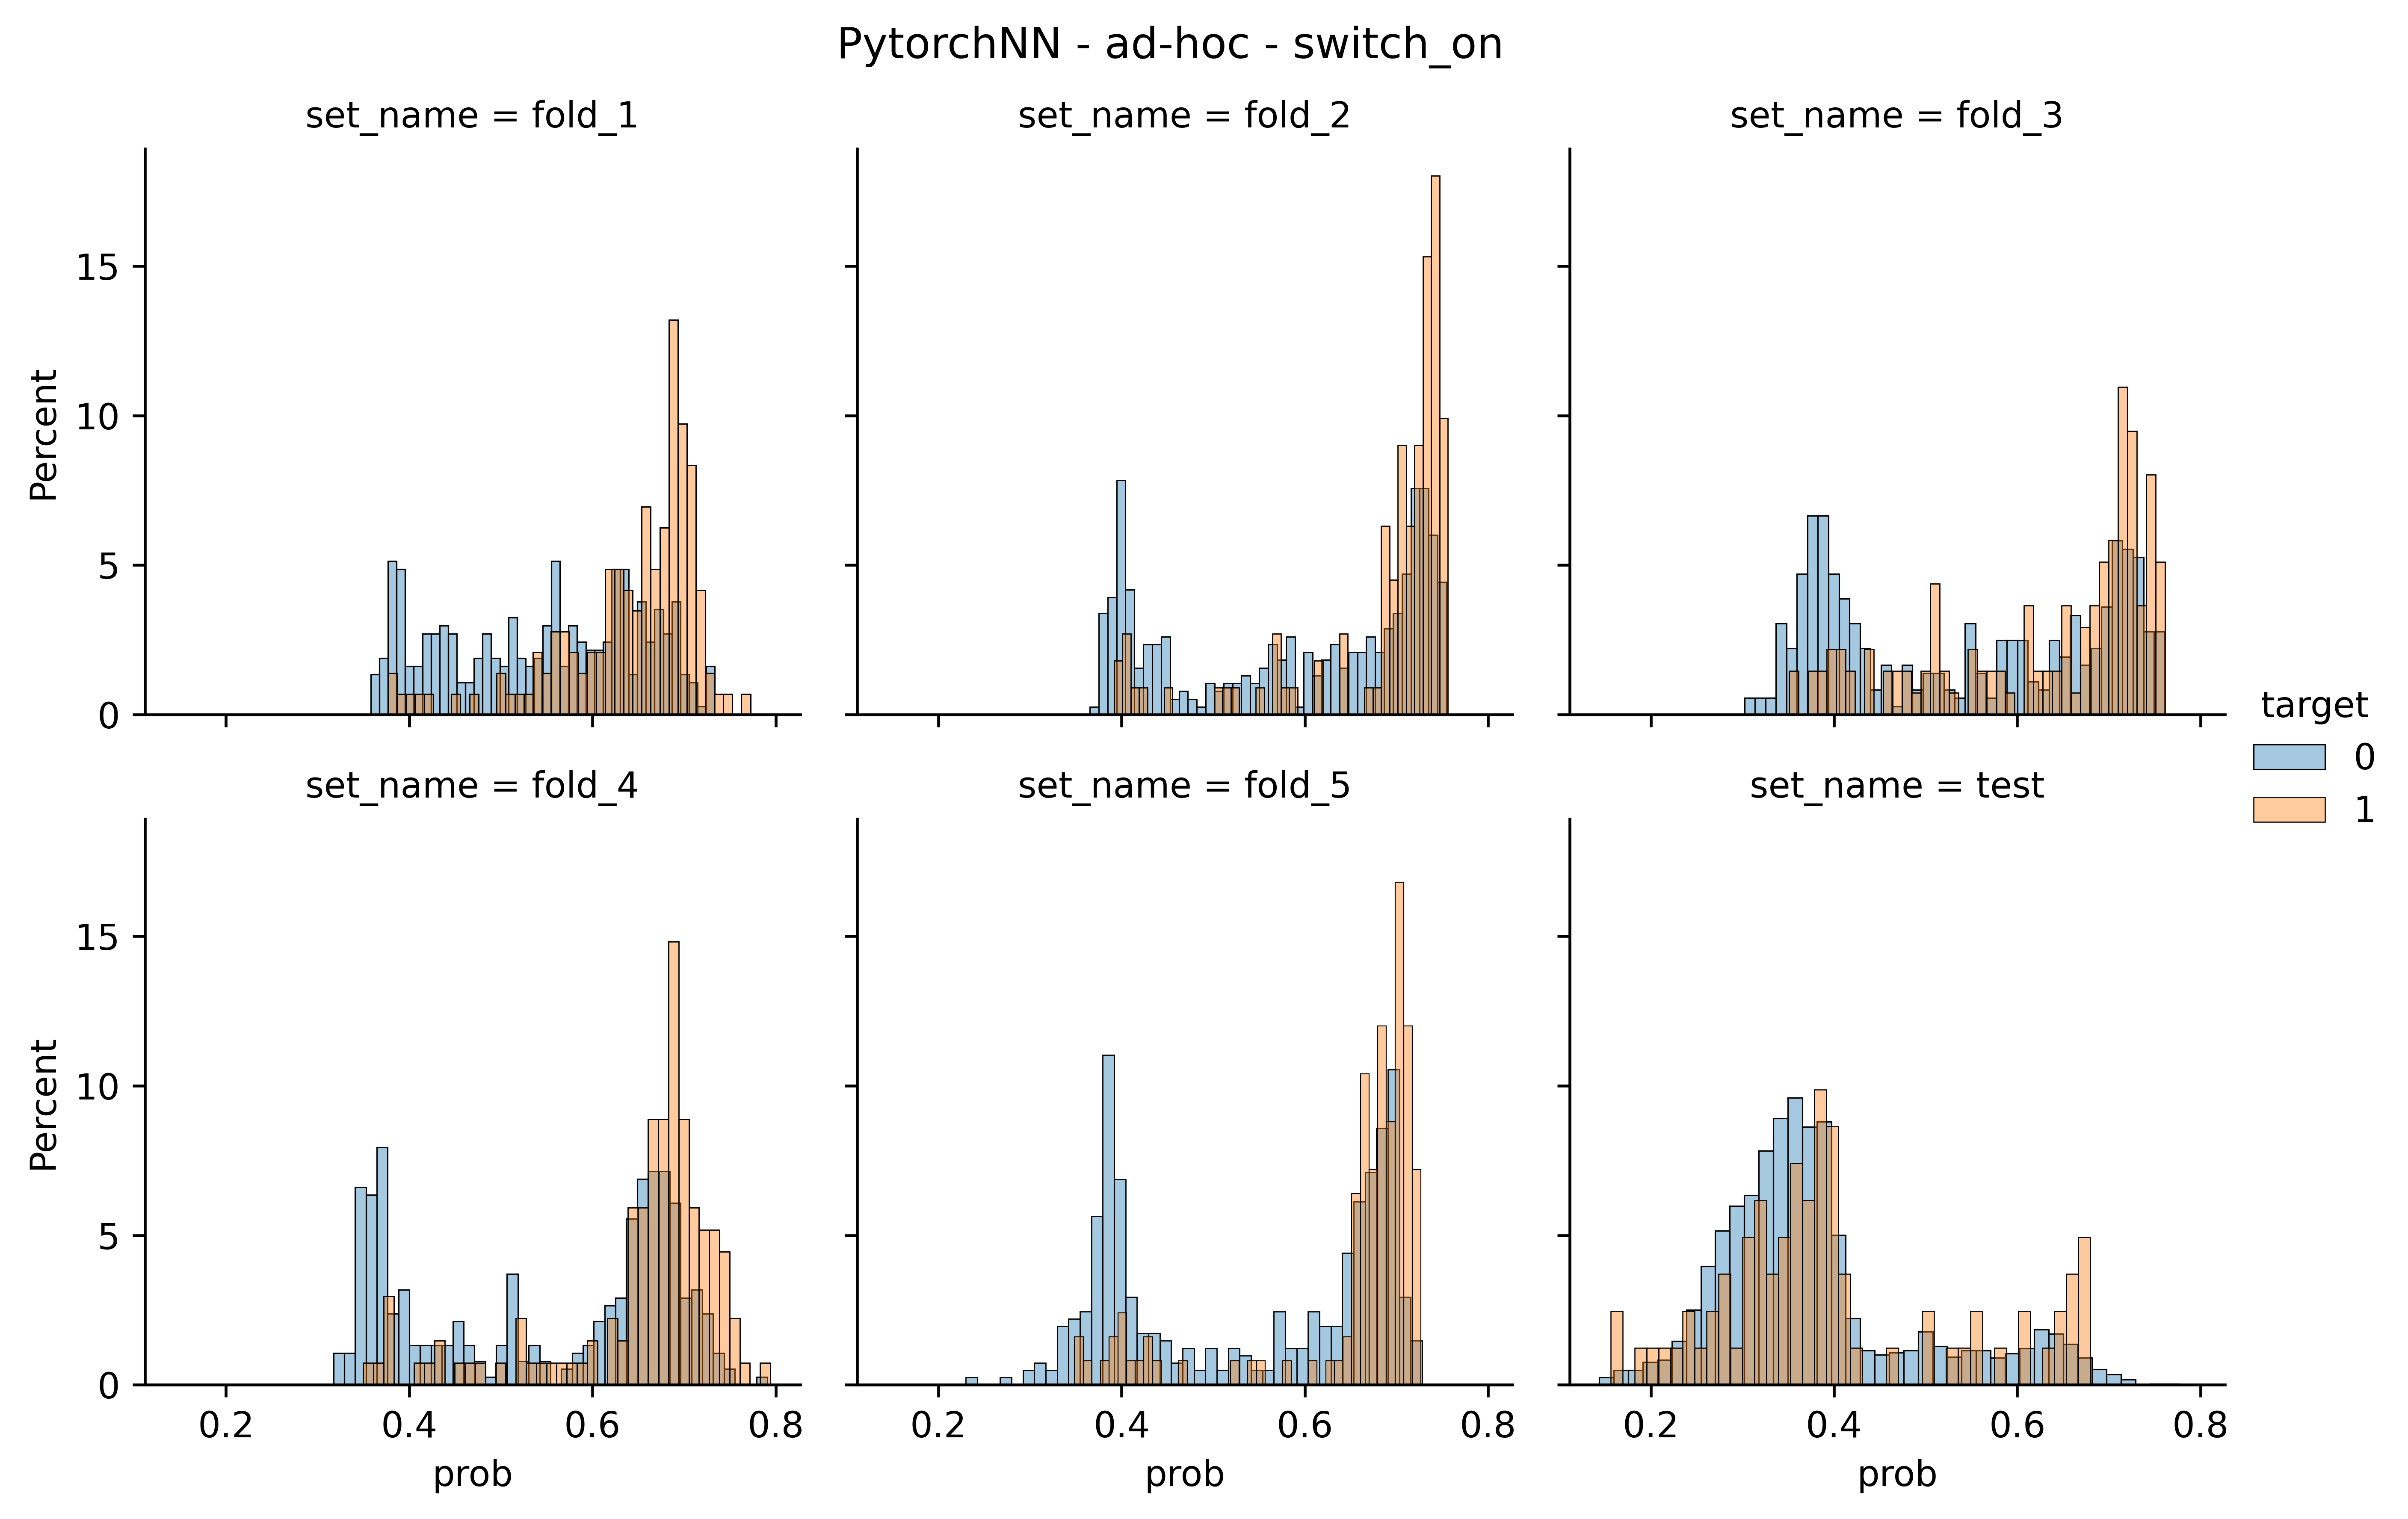
\includegraphics[width=\linewidth]{figures/results/ad-hoc/nn/switch_on/2021-12-06_18.44.35.478500__distplot.png}
    \end{subfigure}
    \caption{Ad-hoc switch\_on}
\end{figure}

\begin{figure}
    \centering
    \begin{subfigure}[b]{0.83\textwidth}
    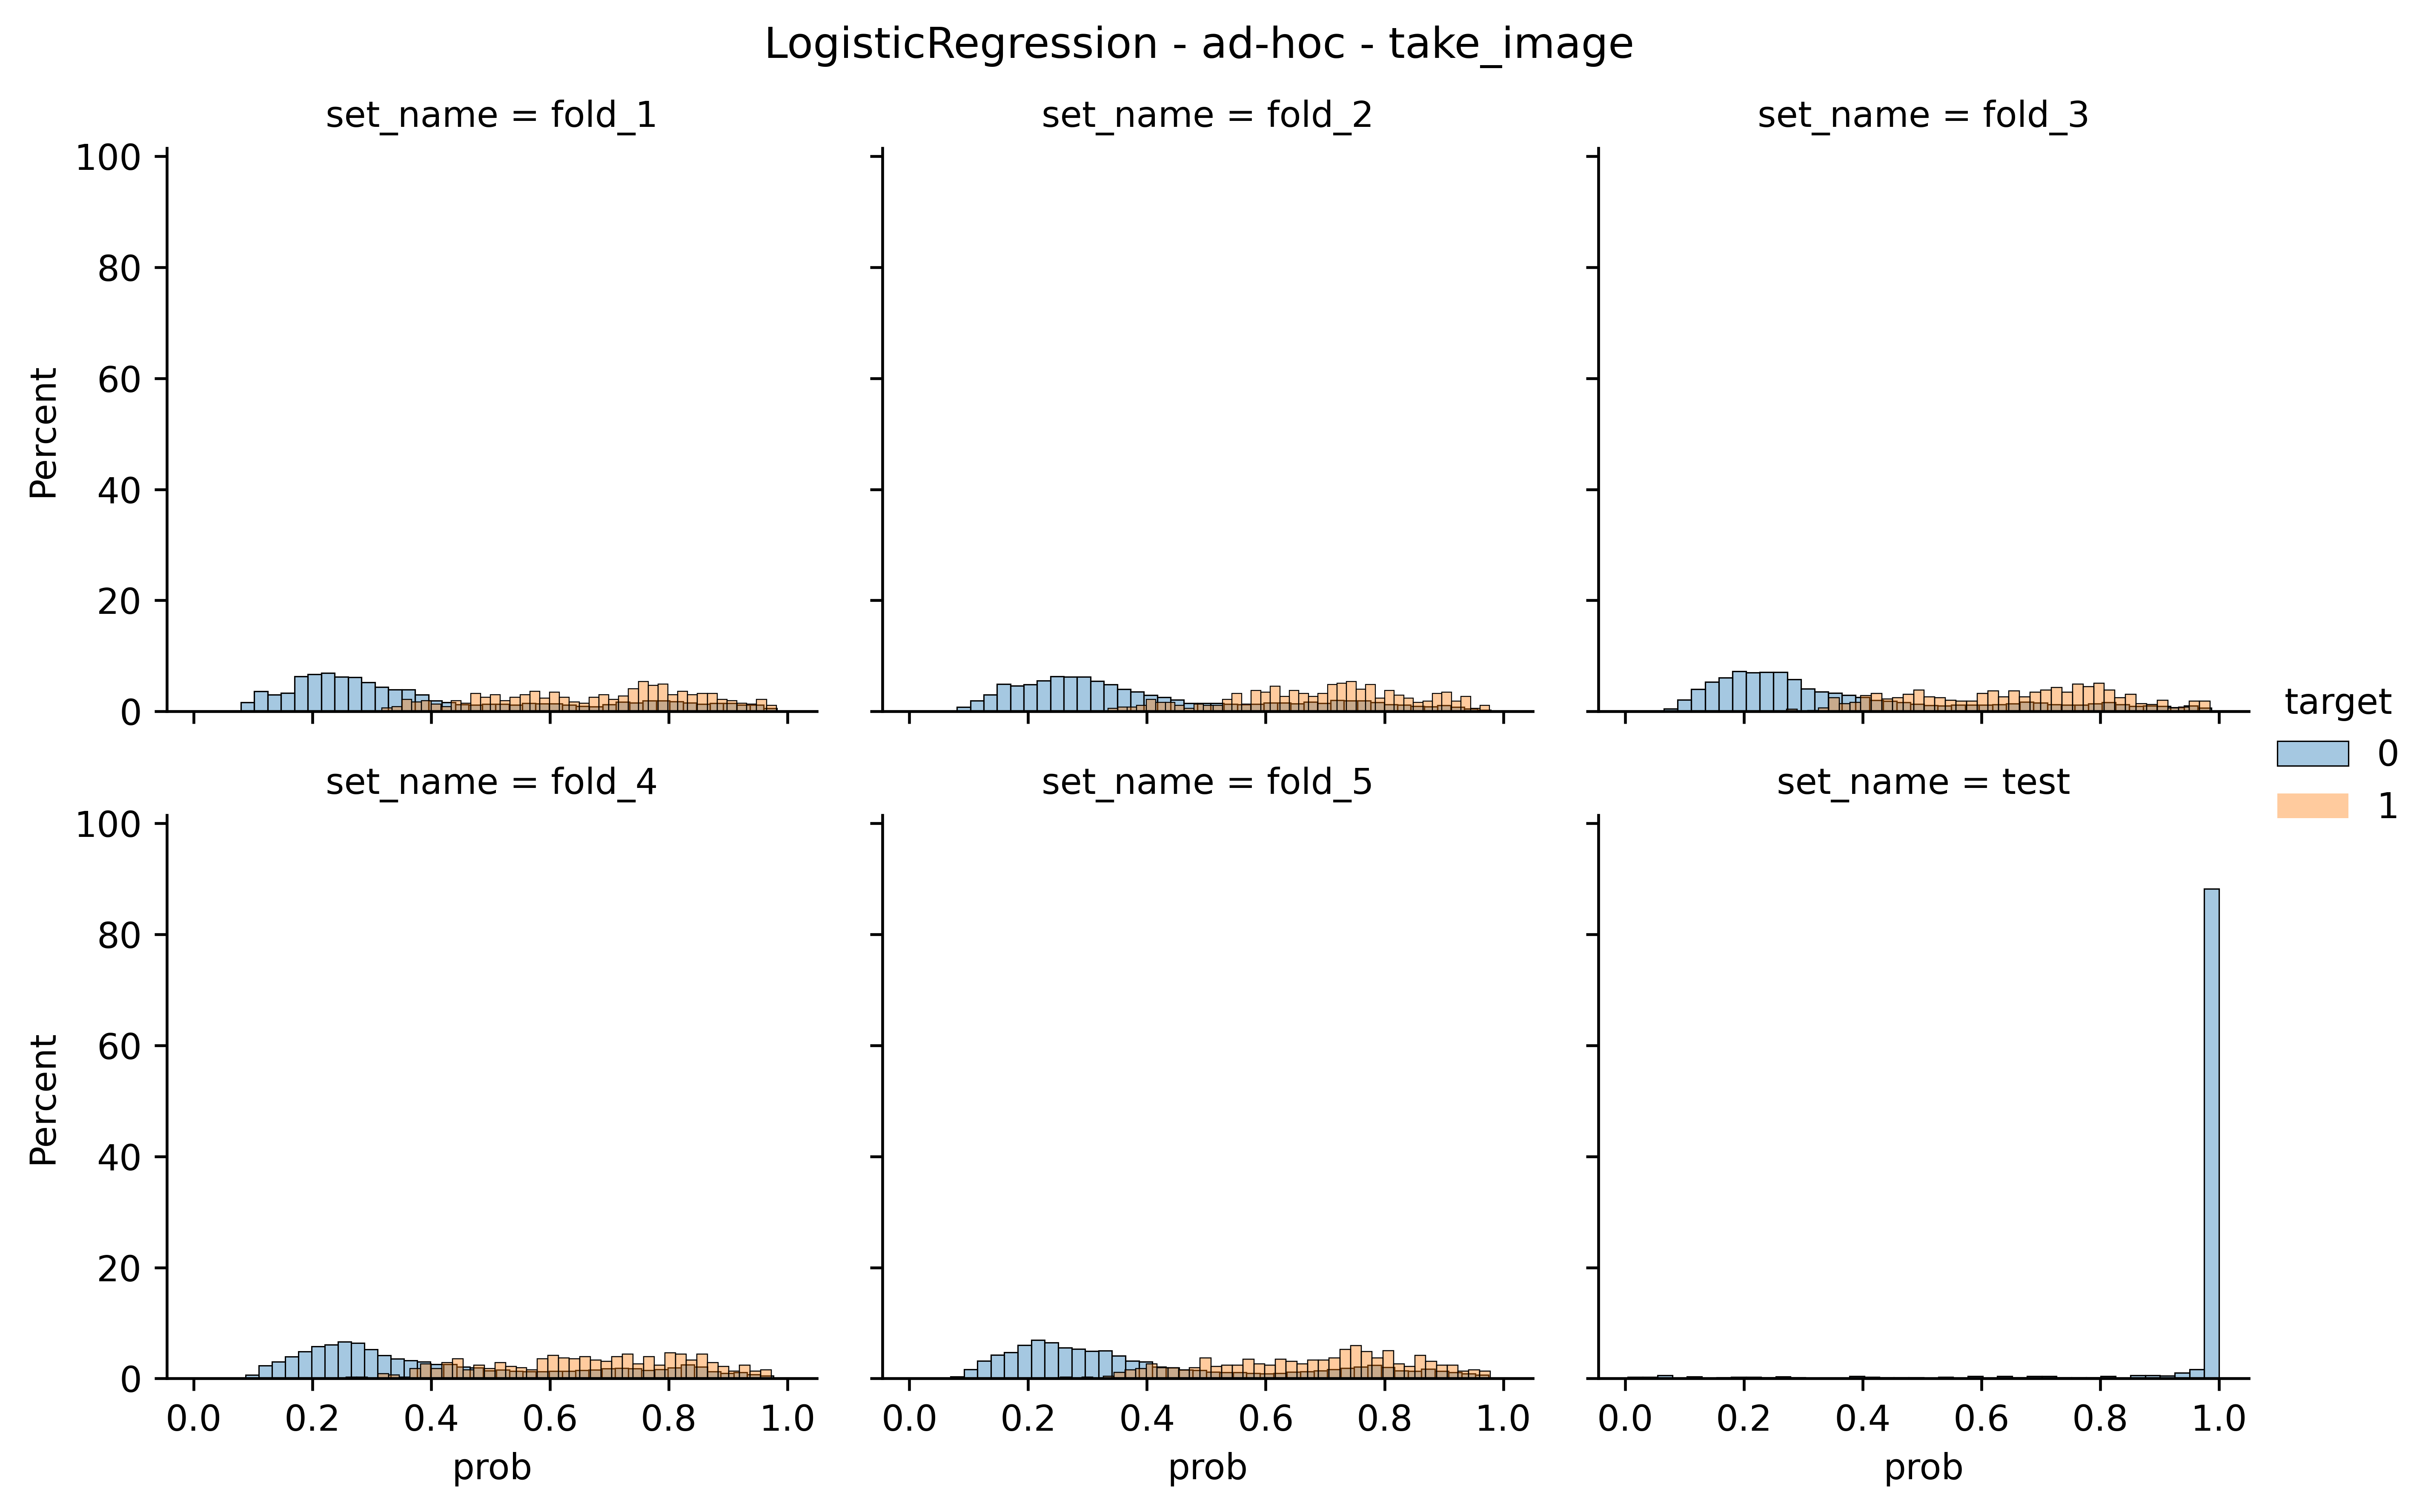
\includegraphics[width=\linewidth]{figures/results/ad-hoc/lgr/take_image/take_image__distplot.png}
    \end{subfigure}
    \hfill
    \centering
    \begin{subfigure}[b]{0.83\textwidth}
        \centering
        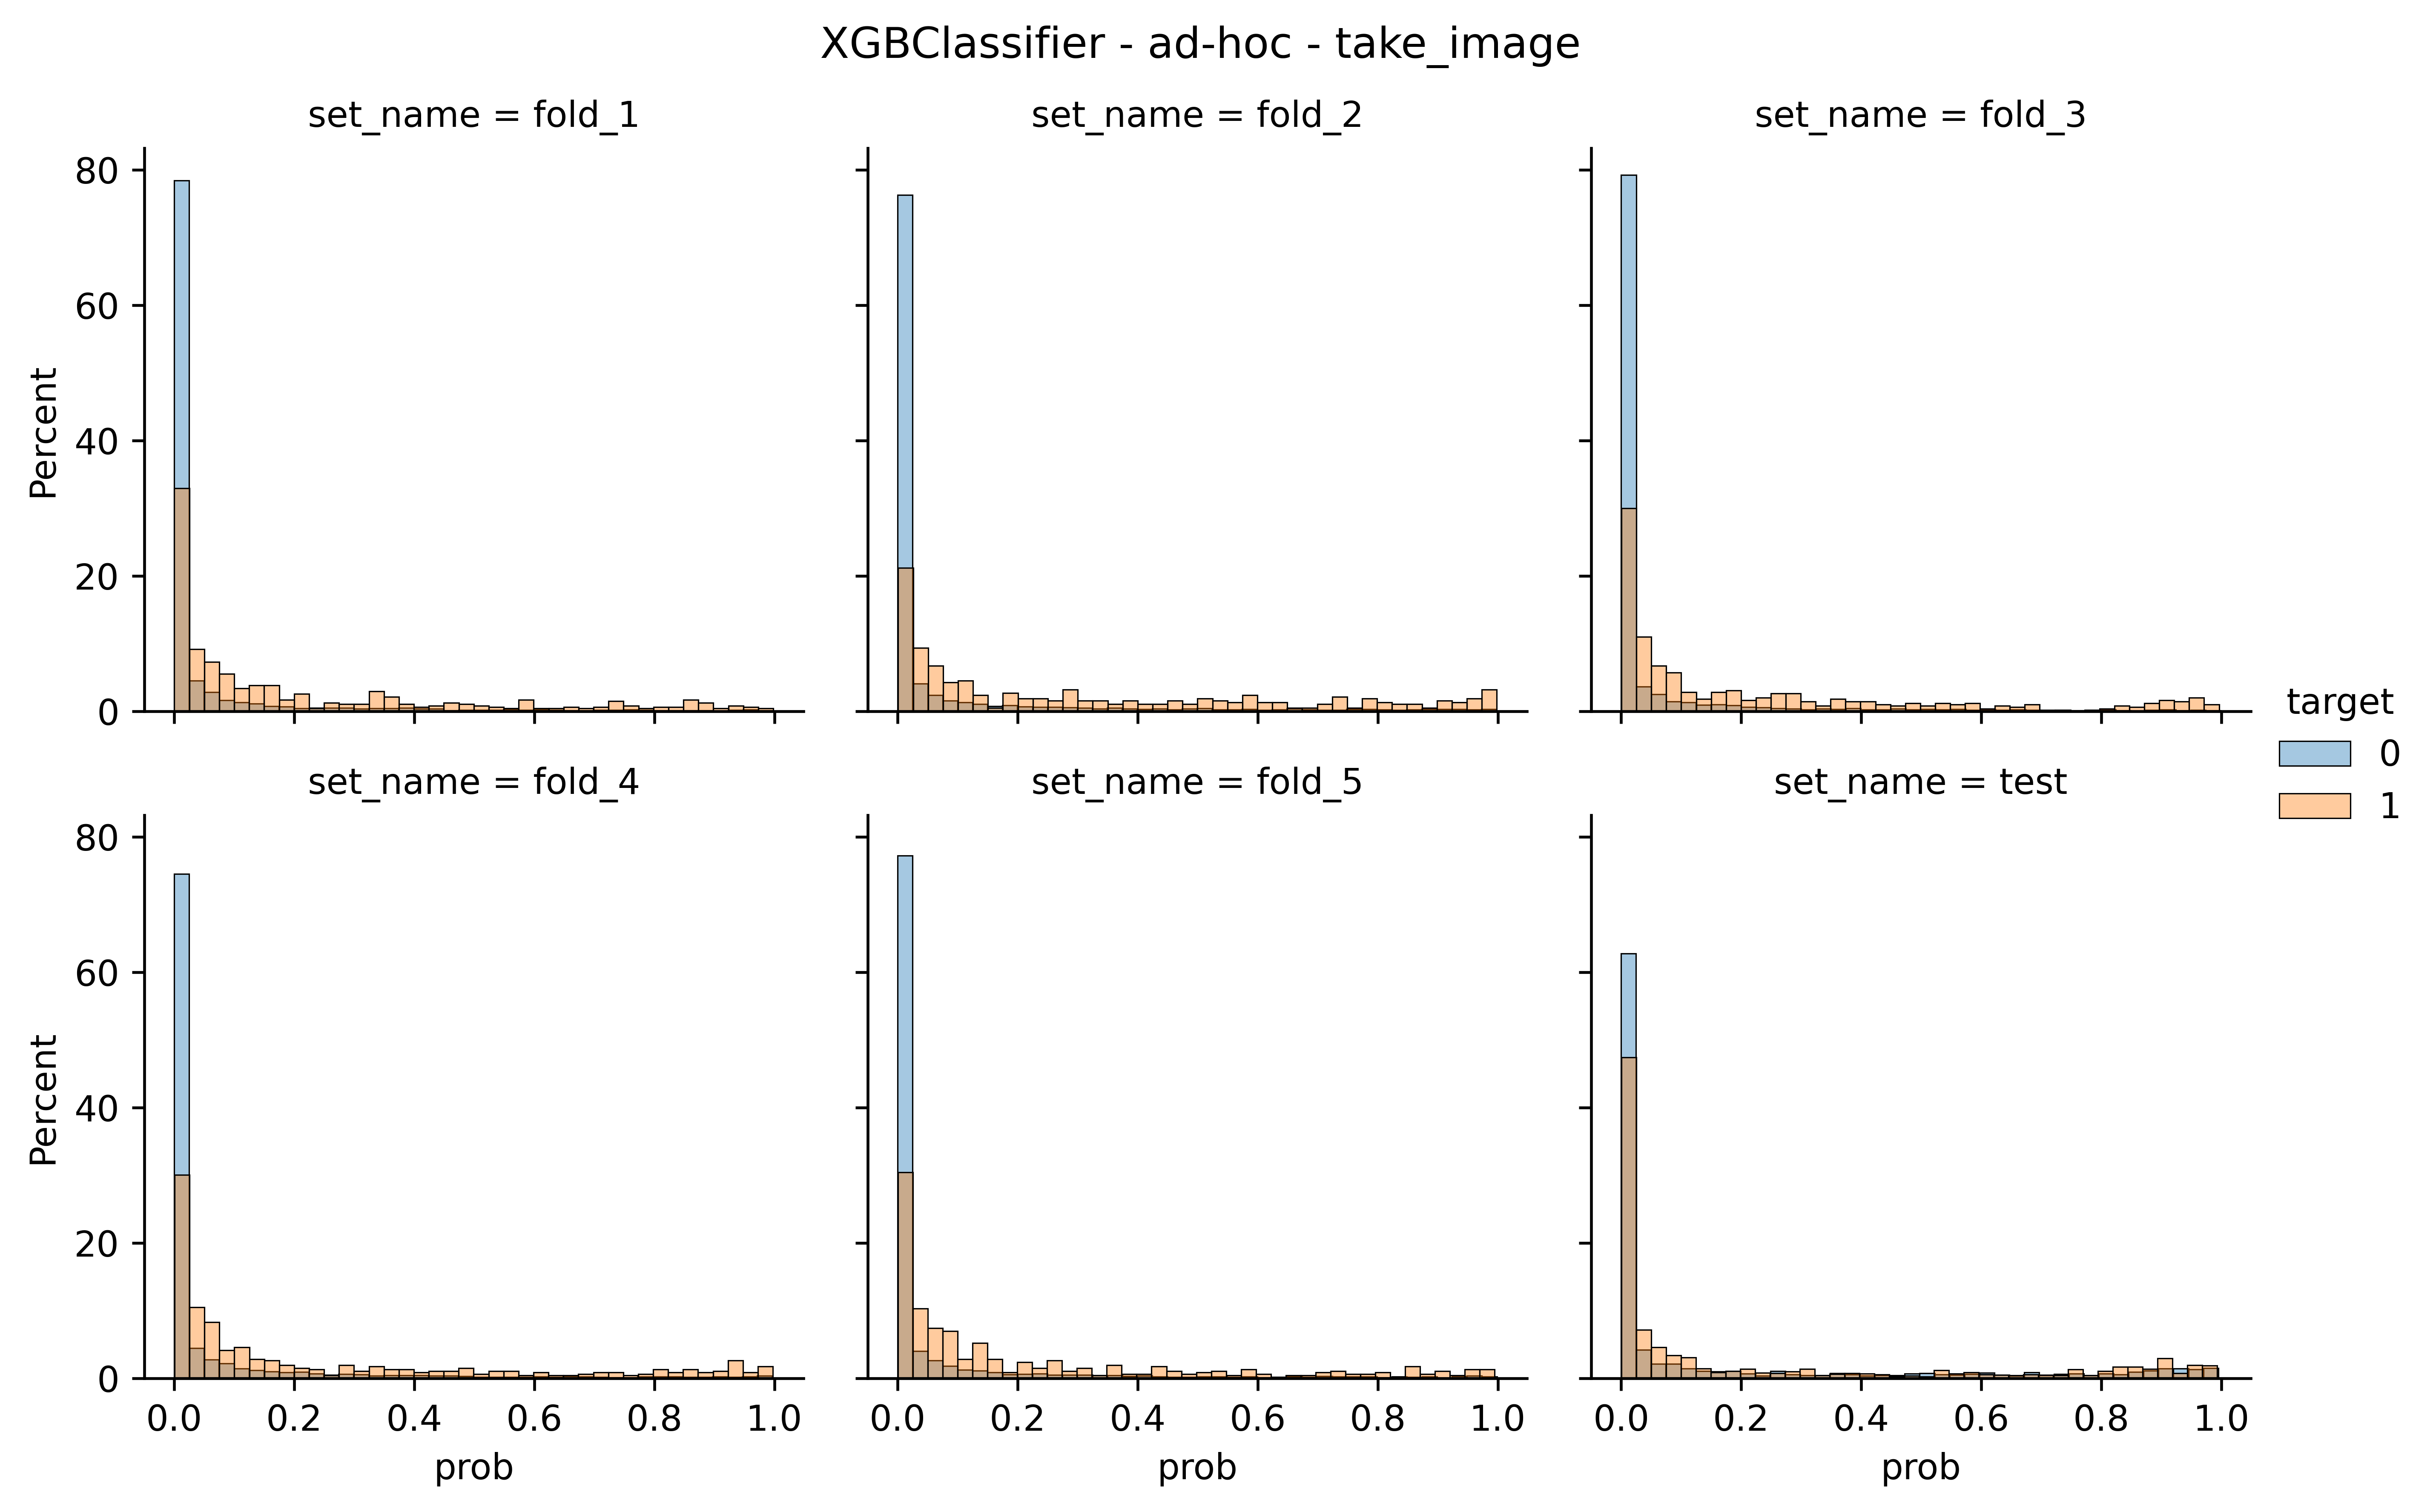
\includegraphics[width=\linewidth]{figures/results/ad-hoc/xgb/2021-12-07_07.38.35.967776__distplot.png}
    \end{subfigure}
    \caption{Ad-hoc take\_image}
\end{figure}

\section{Comparación de mejores modelos}
\label{results:comparison}

\section{Tiempos de predicción}
\label{exp:time}

Para un nuevo ejemplo no visto se debe realizar el proceso completo creación de ventanas, codificación, predicción por parte del clasificador, y posterior agrupamiento de ventanas para obtener la máxima prioridad. Al incluir los modelos predictivos en el proceso de grounding heurístico el tiempo necesario para realizar todas las etapas y obtener el valor de salida del modelo predictivo es importante durante el proceso de grounding heurístico ya que los planificadores deben encontrar la solución a la tarea asignada de acuerdo a un tiempo límite, si este es excedido, ocurre una falla por parte del planificador. Esto motivo la medición del tiempo de respuesta para los modelos predictivos comparados en la sección \ref{results:comparison}.

Actualmente la implementación de grounding heurístico en Fast Downward, son realizadas a nivel de ejemplo. Por lo que la unidad de medida utilizada fueron \emph{ns/ejemplo}, no obstante también se probaron realizar las predicciones a nivel de batch con el de determinar que tan prometedor es incluir este cambio en el algoritmo de grounding heurístico.

\subsection{Predicciones por batch}

\subsection{Predicciones por acción}

\section{Otros experimentos}

Los experimentos presentados en las secciones \ref{exp:ad-hoc}, \ref{exp:wb}, y \ref{exp:time} fueron aquellos principales y los que nos enfocamos durante la tesis. No obstante, se intentaron otras vías de análisis que llevaron a 4 experimentos con el fin de lograr aquel modelo que nos permita guiar el proceso de grounding. A pesar de no lograr resultados concretos fueron parte importante del trabajo y otorgaron conocimiento invaluable para involucrarse más en el dominio del problema.

\subsection{Modelos End-to-end}

End-to-end (E2E) models refieren a sistemas complejos representados por un único modelo neuronal profundo ensamblando las capas de preprocesamiento y como capas intermedias del modelo. En particular, este tipo de pruebas se realizaron en una etapa temprana de la tesis donde la idea de generar ventanas de planes relajados aún no se había investigado. En particular se experimentaron con modelos E2E de FastText donde agrega una capa neuronal más al modelo de embeddings para que sean utilizados en clasificación.
No obstante se optó por descontinuar estos experimentos al comenzar ya que fueron experimentos prototipos donde se buscaba verificar la factibilidad del uso de word embeddings en grounding heurístico.

\subsection{El problema de inclusión sobre planes relajados}

Otra estrategía que utilizamos durante el análisis en la generación de ventanas de planes relajados, fue plantear el problema de clasificación binaria como uno multiclase. En lugar de solo 2 clases, manteníamos 4 que representaban la noción de si una acción estaba incluido en el plan relajado y si eran parte de los good operators del problema. Es decir, una ventana de plan relajado $w$ y acción $a$ es etiquetada como:

\begin{itemize}
    \item 0: Si $a$ no es good operator y no pertenece a $w$.
    \item 1: Si $a$ no es good operator y pertenece a $w$.
    \item 2: Si $a$ es good operator y no pertenece a $w$.
    \item 3: Si $a$ es good operator y pertenece a $w$.
\end{itemize}

Luego al agrupar por ventanas y acción, consideramos como predicción final la clase $3$ si al menos una de las ventanas predijo $3$. Caso contrario si para alguna ventana la predicción fue $2$ predicción del agrupamiento es $2$. Y así sucesivamente hasta la clase $0$.

\subsection{Mayorización}

La repetición de ejemplos con etiquetas diferentes puede dificultar el aprendizaje de un modelo, si no son preprocesadas con alguna técnica de mayorización. Es decir, de entre todas las repeticiones del mismo ejemplo pero con distintas clases, mantener una sola replica preservando la etiqueta que haya ocurrido en mayor cantidad. Esta técnica fue aplicada para la codificación por word embeddings, donde una hipótesis para mejorar la separación de los ejemplos de entrenamiento fue asignar la etiqueta mayoritaria para todo los vector de dimensión $D$ (plan relajado, acción) que estén cerca en un rango en $\mathbb{R}^{D}$.

\subsection{Orden de ventanas como características}

Por último otra implementación que se agregó al sistema y que es un patrón configurable de las etapas de ejecución es la posibilidad de mantener el orden en que ocurren las ventanas. Es decir, se tiene

\begin{table}[h!]
\centering
\scalebox{0.9}{
 \begin{tabular}{||c | c | c | c||} 
 \hline
 Plan relajado & Orden de ventana & Acción & Etiqueta \\ [0.5ex] 
 \hline\hline
 %(take_image satellite0 planet5 instrument1 image1)
 {}[] & 1 &{}[] & 1 \\
 {}[] & 2 &{}[] & 1 \\
 {}[] & 3 &{}[] & 1  \\
 ... & ... & ... & ...\\ [1ex] 
 \hline
 \end{tabular}}
 \caption{Ejemplos etiquetados a partir de un plan relajado y una acción}
 \label{tb:matrix_shape}
\end{table}

El objetivo de este agregado es evitar perder la información del orden durante la separación y se buscaba analizar si es un factor relevante para el entrenamiento y evaluación.